\documentclass[FM,BP]{tulthesis}
% tento dokument používá balíky specifické pro XeLaTeX a lze jej přeložit
% jen XeLaTeXem, nemáte-li instalována použitá (komerční) písma, změňte
% nebo vymažte příkazy \set...font na následujících řádcích
\newcommand{\verze}{1.10}

\usepackage{polyglossia}
\setdefaultlanguage{czech}
\usepackage{xevlna}
\usepackage{graphicx}
\usepackage{placeins}

\usepackage{xcolor}
\usepackage{rotating}
\usepackage{multirow}
\usepackage{colortbl}
\usepackage{hhline}

\usepackage{array}
\usepackage{makecell}

\renewcommand\theadalign{bc}
\renewcommand\theadfont{\bfseries}
\renewcommand\theadgape{\Gape[4pt]}
\renewcommand\cellgape{\Gape[4pt]}

\usepackage{makeidx}
\makeindex

% fonty
\usepackage{fontspec}
\usepackage{xunicode}
\usepackage{xltxtra}
% \setmainfont[Mapping=tex-text,BoldFont={* Bold},Numbers=OldStyle]{Baskerville 10 Pro}
% \setsansfont[Mapping=tex-text,BoldFont={* Bold},Numbers=OldStyle]{Myriad Pro}
% \setmonofont[Scale=MatchLowercase]{Vida Mono 32 Pro}



% po revizi odstranit, LM, start
\setlength{\marginparwidth}{2cm} 
\usepackage{todonotes} 
\newcommand{\note}[1]{\todo[color=blue!40]{#1}}
\newcommand{\change}[1]{\todo[color=red!40]{#1}}
\newcommand{\extend}[1]{\todo[color=green!40]{#1}}
% po revizi odstranit, LM, end



% příkazy specifické pro tento dokument
\newcommand{\argument}[1]{{\ttfamily\color{\tulcolor}#1}}
\newcommand{\argumentindex}[1]{\argument{#1}\index{#1}}
\newcommand{\prostredi}[1]{\argumentindex{#1}}
\newcommand{\prikazneindex}[1]{\argument{\textbackslash #1}}
\newcommand{\prikaz}[1]{\prikazneindex{#1}\index{#1@\textbackslash #1}}
\newenvironment{myquote}{\begin{list}{}{\setlength\leftmargin\parindent}\item[]}{\end{list}}
\newenvironment{listing}{\begin{myquote}\color{\tulcolor}}{\end{myquote}}
\sloppy

% deklarace pro titulní stránku
\TULtitle{Rozpoznávání emocí v audio nahrávkách s využitím hlubokých neuronových sítí}{}
\TULauthor{Tomáš Petříček}

% pro bakalářské, diplomové a disertační práce
\TULprogramme{B2646}{Informační technologie}{Information technology}
\TULbranch{1802T007}{Informační technologie}{Information technology}
\TULsupervisor{Ing. Lukáš Matějů, Ph.D.}
\TULyear{2021}

% Vložil Koprnický, použití bibLateXu
% BibLaTeX settings
\usepackage[ 
backend=biber
%,style=iso-authoryear
,style=iso-numeric
%,style=numeric
%,sortlocale=cs_CZ
,autolang=other
,bibencoding=UTF8
%,urldate=edtf
]{biblatex}
\addbibresource{citations.bib} % vložení seznamu literárních zdrojů v bib formátu / input of references in bib format

%%%%%%%%%%%%%%%%%%%%%%%%%%
% Formátování podle pokynů FZS, čárka mezi jmény a poslední jméno se spojkou „a“
% při volbě iso-authoryear, 
\DeclareDelimFormat{multinamedelim}{\addcomma\space}

\DeclareDelimFormat{finalnamedelim}{%
  \ifnumgreater{\value{liststop}}{2}{\finalandcomma}{}%
  \addspace\bibstring{and}\space}

\DeclareNameAlias{author}{family-given/given-family} 
% kulaté závorky kolem citačního záznamu použitím \parencite{}
% nebo použitím standardního příkazu \cite{} s touto redefinicí \let\cite\parencite
%%%%%%%%%%%%%%%%%%%%%%%%%%

% Hranaté závorky kolem čísel v seznamu literatury při použitém iso-numeric
\DeclareFieldFormat{labelnumberwidth}{\mkbibbrackets{#1}}

\usepackage{csquotes} %užití biblatexu hlasí warnings, důvodem může být použití českých uvozovek v citacích! / solving of problems with Czech quotations
\urlstyle{same} %sazba url odkazů stejným fontem jako ostatní text, řešení problémů v zalamování hypertextových odkazů v citacích / url in references seting into the same form as text 

\begin{document}

\ThesisStart{male}
%\ThesisStart{zadani-a-prohlaseni.pdf}

\begin{abstractCZ}  % Grammer checked
Bakalářská práce se věnuje rozpoznávání emocí v audio nahrávkách s využitím hlubokých neuronových sítí. V úvodní části je čtenář seznámen s motivací a využitím systému pro rozpoznávání emocí. Na začátku první kapitoly jsou definovány pojmy emoce a rozpoznávání emocí. Navazující podkapitoly jsou zaměřeny na vývoj systému pro rozpoznávání emocí. Další kapitola je věnována seznámení se základy neuronových sítí. Je uveden model používaný v experimentální části práce, vysvětleno trénování a vyhodnocení modelu. V následující části je popsán návrh a práce s balíčkem pro rozpoznávání emocí napsaném v jazyce Python. Poslední kapitola představuje experimenty provedené na datové sadě získané sjednocením datových sad RAVDESS, TESS, SAVEE a EMOVO. Pro klasifikaci byla použita neuronová síť typu MLP. Byla implementována a natrénována pomocí frameworku PyTorch. MFCC příznaky byly zvoleny pro učení modelu. Provedené experimenty byly zdokumentovány a rozebrány. V závěru práce jsou shrnuty výsledky a navrženy metody pro dosažení lepších výsledků.
\end{abstractCZ}

\begin{keywordsCZ}
rozpoznávání emocí z řeči, strojové učení, neuronové sítě, PyTorch, MFCC
\end{keywordsCZ}

\todo[inline,color=green!40]{přidal bych přesné hodnoty pro finální model, ať rovnou ukazuješ, že to funguje}

\vspace{2cm}

\begin{abstractEN}
Bachelor's thesis deals with emotion recognition in audio recordings using deep neural networks. In the introductory part, the reader is familiarized with the motivation and application of speech emotion recognition system. At the beginning of the first chapter, the concepts of emotion and emotion recognition are defined. Subsequent sections are focused on the development of a speech emotion recognition system. Next chapter is devoted to acquaintance with the basics of neural networks. Model used in the experimental part of the work is presented, training and evaluation of the model are explained. The following section describes the design and workflow of emotion recognition package written in Python. The last chapter presents experiments performed on a dataset obtained by unifying the RAVDESS, TESS, SAVEE and EMOVO datasets. An MLP neural network was used for classification. It was implemented and trained using the PyTorch framework. MFCC features were selected for model learning. Performed experiments were documented and analyzed. At the end of the work, the results are summarized and methods for achieving better results are proposed.
\end{abstractEN}

\begin{keywordsEN}
speech emotion recognition, machine learning, neural networks, PyTorch, MFCC
\end{keywordsEN}

\clearpage

\begin{acknowledgement}
Jako první bych chtěl poděkovat vedoucímu této práce panu doktoru Lukáši Matějů za důsledné vedení, pravidelné konzultace a užitečné rady.
\end{acknowledgement}

\note{Seznam nebýt v obsahu}
\tableofcontents

\renewcommand{\listfigurename}{Seznam obrázků}
\renewcommand{\listtablename}{Seznam tabulek}

\thispagestyle{empty}
\listoffigures
\listoftables

% \clearpage
% \begin{abbrList}
% \textbf{MFCC} & Melovské frekvenční kepstrální koeficienty
% \end{abbrList}

\chapter{Úvod} % Grammer checked
Řeč je naše nejpřirozenější forma komunikace a emoce nám pomáhají si lépe porozumět. Díky emocím můžeme svému okolí ukázat svůj vnitřní psychický stav. Při používání jiných forem komunikace je těžší vyjádřit své emoce, přesto lidé našli způsoby, jak je do komunikace zapojit. S rozvojem chatovácích platforem byly vyvinuty smajlíky, které reprezentují zjednodušený výraz lidského obličeje. Můžeme, tak ve zprávě poslat úplnější informaci a lépe si porozumět~\cite{DBLP:journals/speech/AkcayO20}.

Nicméně i přesto, že jsme schopni vyjádřit své emoce, tak to neznamená, že se pochopíme. Emoce jsou subjektivní a každý z nás je může vnímat trochu jinak. Tato vlastnost emocí neusnadňuje ani vývoj systémů pro jejich rozpoznávání. Zatím nebyl nalezen způsob, jak emoce měřit. Proto lidé usilují o vyvinutí systémů schopných rozpoznávat emoce bez explicitně zadaných instrukcí.

Modely strojového učení jsou schopné najít skryté vzory v datech a naučit se je rozdělovat. Pro učení modelu pro rozpoznávání emocí lze použít data získaná z textu, změn výrazu tváře, hlasu, gest nebo držení těla~\cite{konar_chakraborty_2015}. Modely založené na rozpoznávání emocí z řeči mohou najít uplatnění na příklad při vývoji virtuálních asistentů.

V posledních letech došlo k rozvoji osobních virtuálních asistentů jako jsou Siri a Alexa, které jsou používány pro hlasové ovládání elektronických zařízení. Mohou odesílat textové zprávy, přijímat telefonní hovory, přehrávat hudbu nebo vyhledávat ve webovém prohlížeči. Systém schopný rozpoznávat emoce může zlepšit komunikaci s asistentem tak, aby se nám zdála přirozenější~\cite{DBLP:journals/corr/abs-1912-10458}.

Dále může model najít uplatnění pro call centra. Data generovaná call centrem mohou posloužit k vývoji automatické obsluhy zákazníků nebo pro optimalizaci práce v call centru. Dispečerovi můžou být, podle emocionálního stavu zákazníka, nabídnuty scénáře, podle kterých je vhodné v dané situaci postupovat. Model může být využit také k vylepšení systémů doporučující videa nebo podcasty. Uplatnění může najít také při vývoji realističtějších her. Zdroje dat jsou různé. V dnešní době převažují uměle vytvořené datové sady~\cite{konar_chakraborty_2015}.

Práce se zabývá aktuálním tématem a výsledky mohou vést k rozšíření systémů vyvíjených Laboratoří počítačového zpracování řeči (SpeechLab)~\cite{speechlab}. Model by se mohl implementovat na příklad do monitorovacího systému pro přepis TV a radio streamů v různých jazycích.

\chapter{Základy rozpoznávání emocí}

\section{Emoce} % Grammer checked
V současnosti není zvolena jednotná definice emocí. Existuje jich mnoho. Emoce popisují náš vnitřní stav a jejich tvorba je ovlivněna mnoha faktory, jako je osobní zkušenost, fyzické, jednací a komunikační reakce. Pro úlohu rozpoznávání emocí je důležité vědět, jak lze emoce rozdělit~\cite{DBLP:journals/speech/AkcayO20}.

Emoce můžeme dělit dvěma způsoby podle diskrétního modelu nebo prostorového modelu. Diskrétní model rozděluje emoce do kategorií. Mezi hlavní kategorie patří: smutek, radost, strach, hněv, znechucení a překvapení. Prostorový model dělí emoce do jednotlivých prostorů jako jsou mocenství, vzrušení nebo vliv. Vzrušení udává sílu emoce a má rozsah od znudění k nadšení. Výhodou diskrétního modelu je, že na rozdíl od prostorového modelu je intuitivnější~\cite{DBLP:journals/speech/AkcayO20}.

\section{Rozpoznávání emocí} % Grammer checked
Postup vývoje systému pro rozpoznávání emocí z řeči je znázorněn na obrázku \ref{fig:ser_pipeline}. Při vývoji typického systému pro rozpoznávání emocí z řeči je nejprve vybrána anotovaná datová sada. Data ze sady jsou nejdříve předzpracována. Dále jsou z nich vytaženy příznaky pro rozpoznávání a jsou z nich vybrány nejvhodnější pro rozpoznávání. Pomocí anotovaných příznaků lze natrénovat model strojového učení z kategorie učení s učitelem. Výsledný model je buď typu klasifikátor, pokud jsou emoce děleny diskrétně nebo regresor v případě, že jsou děleny prostorově. Výsledkem klasifikace nebo regrese jsou předpovědi~\cite{konar_chakraborty_2015}.

\begin{figure}[htbp]
\centerline{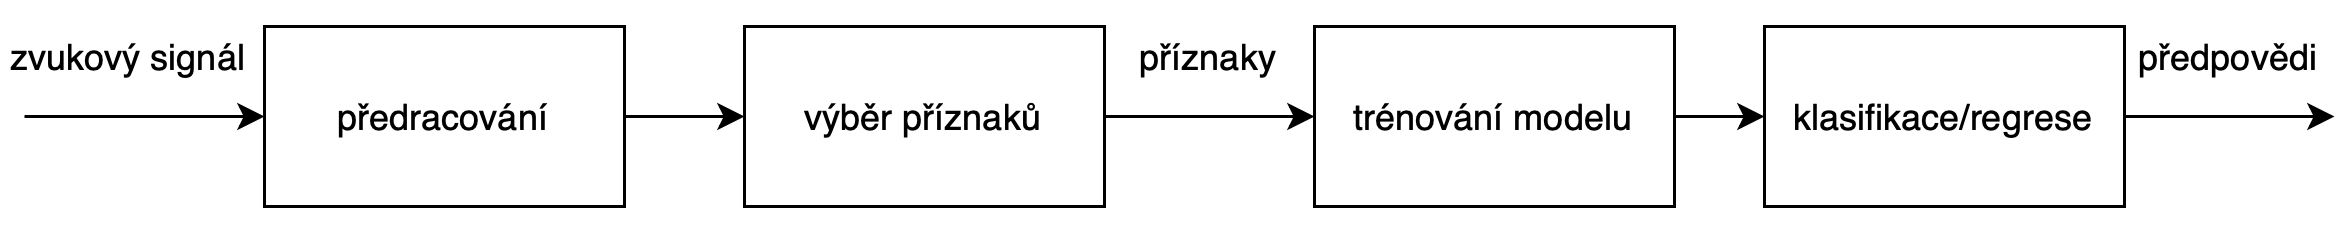
\includegraphics[width=\textwidth,height=\textheight,keepaspectratio]{speech_emotion_recognition-pipeline.png}}
\caption{Postup při rozpoznávání emocí}
\label{fig:ser_pipeline}
\end{figure}
\FloatBarrier

\section{Současné poznání}
Při rozpoznávání emocí z řeči není určeno, které emoce rozpoznávat a jestli pro rozpoznávání používat diskrétní nebo prostorový model. Nicméně při použití diskrétního modelu jsou vymezeny takzvané velké n emoce mezi než patří na příklad: hněv, strach, smutek nebo radost~\cite{konar_chakraborty_2015}.

V současné době existuje mnoho datových sad. Datové sady se od sebe liší především vznikem, počtem emocí a jazykem. Podle způsobu vzniku jsou datové sady děleny na předstírané, vybuzené a přirozené. Mezi hojně používané předstírané datové sady patří Danish Emotional Speech dataset (DES)~\cite{DBLP:conf/interspeech/EngbergHAD97}, Berlin Emotional Speech database (BES)~\cite{bes_dataset}, Speech Under Simulated and Actual Stress (SUSAS) database~\cite{DBLP:conf/interspeech/HansenB97} nebo Ryerson Audio-Visual Database of Emotional Speech and Song database (RAVDESS)~\cite{Livingstone2018}. Mezi vybuzené datové sady patří na příklad eNTERFACE~\cite{DBLP:conf/icde/MartinKMP06}. Většina datových sad má do jedné hodiny délky a nahrávky jsou namluveny kolem deseti mluvčích. Nicméně při rozpoznávání řečí je typicky potřeba datová sada s několika sty hodinami nahrávek a větší různorodost mluvčích~\cite{konar_chakraborty_2015}. \note{rozpoznávání řečí? jako jazyků?}

Příznaky používané pro rozpoznávání emocí lze dělit na prozodické, spektrální, založené na kvalitě hlasu nebo příznaky založené na Teagerově energetickém operátoru (TEO). Mezi prozodické příznaky patří na příklad intonace nebo rytmus. K příznakům založených na spektru lze přiřadit Melovské frekvenční kepstrální koeficienty (MFCC), lineární predikční kepstrální koeficienty (LPCC) nebo log-frequency power coefficients (LFPC). Chvění, mihotání nebo poměr harmonie k hluku (HNR) jsou příznaky založené na kvalitě zvuku~\cite{DBLP:journals/speech/AkcayO20}.

Pro rozpoznávání emocí jsou používány buď klasifikátory nebo regresory, podle toho jestli jsou emoce děleny na základě diskrétního nebo prostorového modelu. Z tradičních modelů strojového učení lze pro klasifikaci použít skryté Markovovy modely (HMM), Gaussovské směsné modely (GMM) nebo metodu podpůrných vektorů (SVM). Z řady klasifikárů typu hluboká neuronová síť (DNN) lze použít vícevrstvý perceptron (NLP), konvoluční neuronové sítě (CNN) nebo rekurentní neuronové sítě (RNN)~\cite{DBLP:journals/speech/AkcayO20}.

\chapter{Datové sady} % Grammer checked
K rozpoznávání emocí se používají anotované datové sady. Mohou být děleny podle toho, jak byla data získána na předstírané, vybuzené a přirozené datové sady. Také se mohou lišit tím, kdo je namluvil. Mluvčí mohou být různého věku a pohlaví a mluvit různými jazyky. Datové sady se také odlišují tvrzeními, která byla vyslovena. Počet a kategorie rozpoznávaných emocí mohou být také různé~\cite{DBLP:journals/speech/AkcayO20}.

V tabulce \ref{tab:overview-datasets} je uveden přehled volně dostupných datových sad. Je patrné, že nejvíce datových sad je předstíraných a nejméně je sad vybuzených. Poměrně velké zastoupení mají anglické datové sady.

\section{Předstírané datové sady} % Grammer checked
Data mohla být pořízena předstíráním, kdy herec při nahrávání předstírá, že emoci prožívá. Tento typ datové sady lze získat spoluprací s profesionálními herci nebo z video záznamů filmů a seriálů. Datovou sadu při spolupráci s herci lze relativně snadno sestavit, protože tvůrci mají poměrně velkou kontrolu nad celým procesem. Data získaná tímto způsobem, ale nemusejí odpovídat reálné situaci, a proto existují další dva způsoby získávání datových sad~\cite{konar_chakraborty_2015}.

\section{Vybuzené datové sady} % Grammer checked
Při získávání vybuzených datových sad je mluvčí umístěn do situace, která se velice podobá reálnému životu. Situace jsou většinou vybírány tak, aby odpovídaly potenciálnímu použití~\cite{konar_chakraborty_2015}.

\section{Přirozené datové sady} % Grammer checked
Poslední způsob získávání dat pro rozpoznávání je z přirozené řeči. Data mohou být získána na příklad z rozhovorů z radií, televizních show nebo záznamů z call center. Ačkoli by tato data měla být pro rozpoznávání nejvhodnější, tak je mnohem obtížnější z nich sestavit datovou sadu. Na data se mohou vztahovat právní nároky a je s nimi více práce při zpracování~\cite{DBLP:journals/speech/AkcayO20}.

\begin{sidewaystable}
\centering
\caption{Přehled volně dostupných datových sad}
\resizebox{\textwidth}{!}{\begin{tabular}{|l|c|c|c|c|c|c|}
\hline
\textbf{Název} & \textbf{Jazyk} & \textbf{Počet tříd} & \textbf{Počet mluvčích} & \textbf{Pohlaví mluvčích} & \textbf{Typ} & \textbf{Velikost} \\\hline
RAVDESS                & angličtina    & 5,7 & 24  & obě        & předstíraná & 2452 promluv \\
SAVEE                  & angličtina    & 7   & 14  & můži       & předstíraná & 480 promluv  \\
TESS                   & angličtina    & 6   & 2   & ženy       & předstíraná & 2800 promluv \\
CHEAVD                 & mandariština  & 8   & 238 & obě        & předstíraná & 2600 promluv \\
DES                    & dánština      & 5   & 4   & obě        & předstíraná & 10 min řeči  \\
EESDB                  & mandariština  & 7   & 16  & obě        & předstíraná & 400 promluv  \\
EMA                    & angličtina    & 4   & 3   & obě        & předstíraná & 34 promluv   \\
EMOVO                  & italština     & 7   & 6   & obě        & předstíraná & 588 promluv  \\
eNTERFACE’05           & angličtina    & 6   & 42  & obě        & vybuzená    & 1166 promluv \\
Keio-ESD               & japonština    & 47  & 71  & muži       & předstíraná & 940 promluv  \\
RECOLA Speech Database & francouzština & 7   & 46  & obě        & přirozená   & 1308 promluv \\
SAMAINE Database & angličtina, řečtina, hebrejština & 5          & 150            & není známo       & přirozená & 959 konverzací \\
VAM                    & němčina       & 3   & 47  & není známo & přirozená   & 947 promluv  \\
TUM AVIC Database      & angličtina    & 5   & 21  & obě        & přirozená   & 3901 promluv \\
AFEW Database          & angličtina    & 7   & 330 & není známo & přirozená   & 1426 promluv \\
TURES                  & turečtina     & 9   & 582 & obě        & předstíraná & 5100 promluv \\
BAUM-1 Speech Database & turečtina     & 12  & 31  & obě        & předstíraná & 1222 promluv \\
\hline
\end{tabular}}
\label{tab:overview-datasets}
\end{sidewaystable}
\FloatBarrier

\section{Vybrané datové sady}
\subsection{RAVDESS} \label{desc/ravdess} % Grammer checked
RAVDESS~\cite{Livingstone2018} znamená Ryerson Audio-Visual Database of Emotional Speech and Song a označuje anglickou datovou sadu obsahující nahrávky řeči a písní. Spolu s nahrávkami zvuku byly pořízeny i video záznamy mluvčích. Nahrávky byly namluveny 24 herci, z nichž bylo dvanáct žen a dvanáct mužů, což činí datovou sadu pohlavně vyrovnanou. Mluvčí mluvili severoamerickou angličtinou. Nahrávky řeči zachycují osm emocí: klid, radost, smutek, hněv, strach, překvapení, znechucení a neutrální stav. Každý herec namluvil dvě tvrzení ve dvou úrovních emocionální intezity, běžnou a silnou, pro všechny emoce. Namluvené výrazy byly „Kids are talking by the door" a „Dogs are sitting by the door". Počet zvukových nahrávek řeči je celkově 1440 a mají dobu trvání 1,5 hodiny. Každá nahrávka v datové sadě má přiřazenou anotaci, která udává druh nahrávky, druh emoce, emocionální intezitu, tvrzení, číslo opakování a herce, který nahrávku namluvil. Délky nahrávek se pohybují kolem třech minut. Datové sada je dostupná buď na webových stránkách smartlaboratory.org nebo na kaggle.com~\cite{smart_lab}.

\subsection{SAVEE} \label{desc/savee} % Grammer checked
Surrey Audio-Visual Expressed Emotion (SAVEE) označuje anglickou datovou sadu pro rozpoznávání emocí. Obsahuje 480 promluv a má celkovou trvání 0,5 hodiny. Rozlišuje sedm emocí, mezi které patří hněv, znechucení, strach, radost, smutek, překvapení a neutrální stav. Byla namluvena čtyřmi mužskými herci mluvícími britskou angličtinou ve věku mezi 27 až 31 lety. Pro tvorbu datové sady bylo vybráno 15 vět z datové sady Texas Instruments a Massachusetts Institute of Technology (TIMIT). \extend{reference} 
Kromě řeči byla při nahrávání zaznamenána i mimika obličeje mluvčích, kteří na něm měli namalovány modré značky~\cite{savee}.

\subsection{TESS} \label{desc/tess} % Grammer checked
Zkratka TESS~\cite{SP2/E8H2MF_2020} znamená Toronto emotional speech set a označuje anglickou datovou sadu pro rozpoznávání emocí. Obsahuje 2800 promluv, které byly namluveny dvěma herečkami ve věku 26 a 64 let. Má celkovou délku trvání 1,6 hodiny. Rozlišuje sedm emocí mezi něž patří hněv, znechucení, strach, radost, překvapení, smutek a neutrální stav. Každá herečka namluvila 200 promluv pro všechny emoce. Promluva vždy začíná slovy "Say the word" a končí jedním z 200 vybraných slov~\cite{tess}.

\subsection{EMOVO} \label{desc/emovo} % Grammer checked
EMOVO~\cite{DBLP:conf/lrec/CostantiniIPT14} je italská datová sada pro rozpoznávání emocí. Zvukové nahrávky byly vytvořeny šesti herci, z nichž tři byli muži a tři ženy. Každý herec vyslovil 14 vět pro každou emoci. Datová sada rozlišuje sedm emocí, mezi něž patří znechucení, strach, hněv, radost, překvapení, smutek a neutrální stav. Skládá se z 588 promluv a má délku trvání 0,5 hodiny~\cite{DBLP:conf/lrec/CostantiniIPT14}.

\chapter{Předzpracování dat pro rozpoznávání} % Grammer checked 
\note{Předělat pro předzpracování}
Data jsou v typickém systému pro rozpoznávání emocí nejdříve předzpracována. Z dat jsou nejprve vytaženy příznaky na nízké úrovni. \note{tím myslíš co?}
Poté jsou data rozdělena na rámce, z kterých jsou vytaženy příznaky pro rozpoznávání. Dále mohou být na příznaky použity techniky pro snížení počtu příznaků jako je analýza hlavních komponent (PCA) nebo lineární diskriminační analýza (LDA)~\cite{konar_chakraborty_2015}.

\section{Rámcování} % Grammer checked
Rámcování bývá prvním krokem předzpracování dat pro rozpoznávání, kdy je zvukový signál rozdělen na menší časové úseky zvané rámce, které nabývají většinou rozsahu mezi 10\textendash30 milisekundami. Často se jednotlivé rámce překrývají z 30\textendash50 \%, aby se zachoval vztah mezi jednotlivými rámci~\cite{DBLP:journals/speech/AkcayO20}. Důvodem rámcování je, že se emoce v průběhu řeči mohou měnit a rozdělení na menší časové úseky zajistí, že emoce zůstane v rámci jednoho úseku stejná~\cite{konar_chakraborty_2015}.

\section{Okénkování} % Grammer checked
Po rámcování většinou přichází okénkování, kdy je na jednotlivé rámce použita okénkovácí funkce. Snižuje amplitudu signálu na jeho okrajích, a tím snižuje úniky, ke kterým může dojít při použití rychlé Fourierovi transformace (FFT). Pro okénkování lze použít Hammingovu okénkovací funkci~\cite{DBLP:journals/speech/AkcayO20}.

\section{Odstranění ticha} % Grammer checked
Dále mohou být použity techniky pro detekci řeči.
S jejich pomocí lze ze signálu odstranit tichá místa. Mohou být použity metody jako je metoda průchodu nulovou úrovní (ZCR), krátkodobá energie nebo autokorelační metody. ZCR udává míru přechodu signálu z kladných do záporných hodnot nebo naopak, a to v rámci jednoho úseku. Hodnota ukazatele je nízká v místech řeči a vysoká v místech ostatních. Při použití krátkodobé energie dosáhne vysokých hodnot v hlasové části a nízkých hodnotu v částech ostatních. Techniky pro odstranění tichých míst v řeči mohou snížit počet dat a zvýšit jejich přínos pro učení~\cite{DBLP:journals/speech/AkcayO20}.

\section{Normalizace} % Grammer checked
Může být použita také normalizace, která zmírňuje rozdíly v řeči mezi mluvčími a zároveň zachová přenášenou informaci. Normalizace může být použita na více úrovních, na úrovni jednotlivých rámců nebo na úrovni celé datové sady. Nejčastěji se pro normalizaci používá z-normalizace~\cite{DBLP:journals/speech/AkcayO20}.

\note{Opravit podle článku}
\section{Odstranění šumu} % Grammer checked
Dále mohou být použity techniky na odstranění šumu, který se může během nahrávání do záznamu dostat. Lze použít techniky, mezi něž patří nejmenší střední kvadratická chyba (MMSE) a logaritmická spektrální amplituda MMSE~\cite{DBLP:journals/speech/AkcayO20}. \change{to jsou beamformery, které to odhadují na základě MMSE, ne? nepřesně napsané, pokud ano}

\chapter{Výběr příznaků} % Grammer checked
Následuje zvolení vhodných příznaků pro rozpoznávání, kdy jsou z mnoha příznaků vybrány pouze nejvhodnější. Je mnoho příznaků, ale nejsou určeny příznaky, které by se hodily přímo pro rozpoznávání emocí. Ze signálu lze získat jak souhrnné, tak lokální příznaky pro rozpoznávání. Mezi souhrnné příznaky patří střední hodnota, směrodatná odchylka, minimální nebo maximální hodnota. Lokální příznaky lze získat z jednotlivých rámců a zastupují krátkodobé změny v signálu~\cite{DBLP:journals/speech/AkcayO20}.

Příznaky pro rozpoznávání emocí v řeči můžeme dělit na prozodické, spektrální, založené na kvalitě hlasu nebo příznaky založené na Teagerově energetickém operátoru (TEO). Nejčastěji používané příznaky při rozpoznávání emocí v řeči jsou prozodické a spektrální příznaky~\cite{DBLP:journals/speech/AkcayO20}.

\section{Prozodické příznaky}  % Grammer checked
Mezi prozodické příznaky patří na příklad intonace nebo rytmus. Řadí se mezi souhrnné příznaky, protože je lze získat z delších hlasových úseků jako jsou hlásky, slova nebo věty. Mezi používané příznaky patří základní frekvence, energie nebo doba trvání. Energie udává míru změny amplitudy signálu v čase. Emoce jako hněv, štěstí nebo překvapení vykazují zvýšenou energii. Na straně druhé znechucení a smutek vykazují energii nízkou. Základní frekvence se postupně snižuje při projevení hněvu, a naopak stoupá při projevení radosti. Doba trvání potřebná k projevení hněvu je obecně kratší než při projevení smutku~\cite{DBLP:journals/speech/AkcayO20}.

\section{Příznaky založené na spektru}  % Grammer checked
Příznaky založené na spektru jsou získávány pomocí Fourierovy transformace, kdy je signál převeden z oblasti časové do frekvenční. Mohou přinést hlubší porozumění signálu než příznaky prozodické. Příznaky jsou získávány z rámců, na které byla použita okénkovací funkce. Melovské frekvenční kepstrální koeficienty (MFCC) jsou založeny na krátkodobém spektru signálu. Mezi další příznaky patří lineární predikční kepstrální koeficienty (LPCC), logaritmické frekvenční silové koeficienty (LFPC) nebo gammatone frekvenční kepstrální koeficienty (GFCC)~\cite{DBLP:journals/speech/AkcayO20}.

\section{Příznaky založené na kvalitě zvuku}  % Grammer checked
Chvění, mihotání nebo poměr harmonie k hluku (HNR) jsou příznaky založené na kvalitě zvuku. Chvění je měřeno na základě nestálosti frekvence a mihotání je založeno na nestálosti amplitudy. Poměr harmonie k hluku udává poměr mezi hlukem a frekvenčním spektrem samohlásek~\cite{DBLP:journals/speech/AkcayO20}.

\section{Příznaky založené na Teagerově energetickém operátoru}  % Grammer checked
Příznaky založené na Teagerově energetickém operátoru jsou používány k detekci stresu. Využívají změny svalového napětí, které při stresové situaci nastává. V této kategorii předstihují příznaky jako jsou MFCC nebo výška tónu~\cite{DBLP:journals/speech/AkcayO20}.

\section{Vybrané příznaky}
\subsection{Melovské frekvenční kepstrální koeficienty} % Grammer checked
Melovské frekvenční kepstrální koeficienty (MFCC) jsou příznaky používané pro rozpoznávání řeči. Technika převodu zvukového signálu na příznaky MFCC spočívá v provedení několika kroků zobrazených na obrázku \ref{fig:mfcc_pipeline}. 

\begin{figure}[htbp]
\centerline{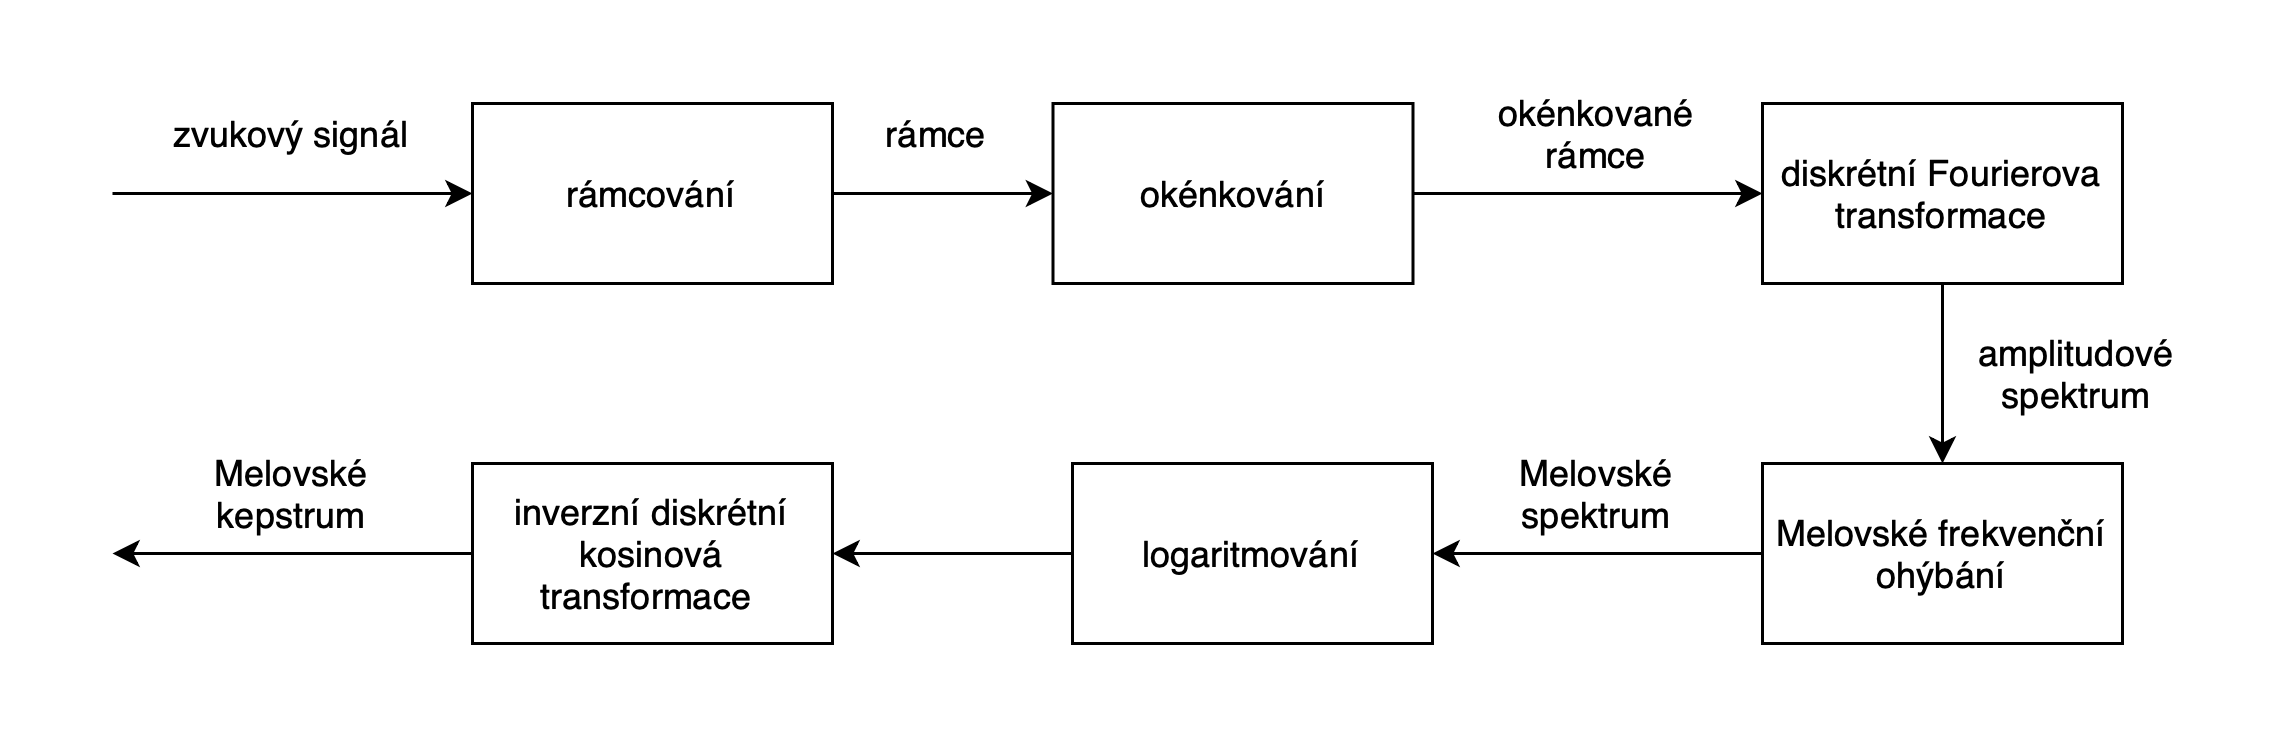
\includegraphics[width=\textwidth,height=\textheight,keepaspectratio]{mfcc_pipeline.png}}
\caption{Postup získání příznaků MFCC}
\label{fig:mfcc_pipeline}
\end{figure}
\FloatBarrier

Při rámcování je zvukový signál nejprve rozdělen na jednotlivé posuvné rámce. Dále je podroben okénkování, kdy je amplituda signálu snížena na konci a na začátku rámce. Může k tomu být použito Hammingovo nebo Hanningovo okénko. Poté je signál převeden pomocí diskrétní Fourierovi transformace (DFT) do frekvenční oblasti. Na výsledné amplitudové spektrum je použito Melovské frekvenční ohýbání. K převodu je použita Melovská banka filtrů složená z trojúhelníkových filtrů s měřítkem v Melovské škále, která zohledňuje vnímaní zvukových frekvencí člověkem. Lidé lépe rozlišují mezi nízkými frekvencemi než mezi vysokými. Dále je signál logaritmován a je provedena inverzní diskrétní kosinová transformace (IDCT). Z koeficientů Melovského kepstra, nazývaných také nulté koeficienty, lze získat koeficienty delta a akcelerační koeficienty (delta delta), které jsou získány použitím první a druhé derivace na nulté koeficienty~\cite{mfcc}.

\note{Přesunout na začátek}
\chapter{Vybrané základy neuronových sítí}
\extend{tady by asi mohlo být zdůvodnění, proč se popisují neuronové sítě}

\section{Způsoby rozpoznávání emocí}  % Grammer checked
\extend{tahle kapitola je taková chudší...?}
Pro rozpoznávání emocí se používají klasifikátory nebo regresory, které spadají do oblasti strojového učení s učitelem~\cite{DBLP:journals/speech/AkcayO20}. Modely strojové učení s učitelem vyžadují označená data. Každý vzorek musí mít přiřazenou anotaci udávající třídu, do které patří. V případě klasifikace jsou to diskrétní třídy, které odpovídají jednotlivým emocím jako jsou na příklad hněv, radost nebo smutek. V případě regrese jsou to desetinné hodnoty, které označují stupeň mocenství, vzrušení nebo dominance většinou v rozsahu od $-1$ do $+1$~\cite{konar_chakraborty_2015}.

\note{poslední dva odstavce popisují už spíše jenom neuronové sítě, které tu ani nejsou zmíněné}
Často se při klasifikaci ke vzorku přidávají i vzorky z okolí pro zvýšení kontextu, který může zlepšit výsledky rozpoznávaní. Důvodem je, že emoce ovlivňují dlouhodobé charakteristiky řeči. Přesný počet rámců, který by se měl vzít není určen. Další způsob, jak klasifikovat emoce je podle statických příznaků jako jsou maximum, minimum nebo časová délka~\cite{konar_chakraborty_2015}.

Při trénování se často používá křížová validace, kdy se mění trénovací a validační sada a je vytvořeno několik modelů, jejichž výsledky jsou zprůměrovány, tím je dosaženo smysluplnějších výsledků. U rozpoznávání emocí je používána především, protože jsou datové sady po většinou menšího rozsahu, a tak má rozdělení do jednotlivých sad větší vliv na výsledek. Jako metrika pro ohodnocení modelu se používá přesnost nebo vážená přesnost, která zohledňuje odlišný počet vzorků pro každou třídu. Přesnost udává pravděpodobnost, že daný vzorek patří do předpovězené třídy~\cite{konar_chakraborty_2015}.

\section{Vícevrstvý perceptron} % Grammer checked
Vícevrstvý perceptron (MLP) neboli dopředná neuronová síť je složena z více lineárních vrstev následovaných nelineárními vrstvami. \note{trochu to zní jako, že první jsou všechny lin a následně všechny nelin}
Lineární vrstva se skládá z parametrů vah a biasů a nelineární vrstva je tvořena aktivační funkcí~\cite{DBLP:books/lib/Bishop07}.

Aby mohla být neuronová síť označena za hlubokou neuronovou síť, musí mít dvě a více lineárních vrstev. První vrstva modelu se nazývá vstupní vrstvou a poslední vrstvou výstupní. Vrstvy mezi vstupní a výstupní vrstvou jsou označovány jako vrstvy skryté. Každá lineární vrstva má svoji šířku, která určuje počet neuronů ve vrstvě. Při klasifikaci do dvou tříd následuje za výstupní vrstvou funkce sigmoida a při klasifikaci do dvou a více tříd funkce softmax.

Jako aktivační funkce ve skrytých vrstvách jsou pro MLP používány nejčastěji funkce sigmoida a ReLU. Neuronovou síť typu MLP lze použít také pro regresi, kdy jsou jako aktivační funkce v nelineárních vrstvách umístěny identity~\cite{DBLP:books/lib/Bishop07}. \extend{možná ilustrační obrázek sítě?}

\section{Trénování} % Grammer checked
Při trénování neuronové sítě je provedena nejprve dopředná propagace následovaná zpětnou propagací. Po zpětném průchodu sítí jsou parametry sítě upraveny pomocí metody největšího spádu, která minimalizuje ztrátu modelu. Jeden proces učení nazýváme epochou.

Při dopředném průchodu lineární vrstvou jsou vstupní příznaky $ y_i $ přeměněny na výstupní příznaky $ x_j $ pomocí lineární kombinace, kterou lze vyjádřit:

\begin{equation}
\label{eqn:linear_layer}
x_j = b_j + \sum_{i}^{N} y_i w_{ij},
\end{equation}

kde proměnná $ i $ odpovídá indexu příznaku z předchozí vrstvy. $ N $ je celkový počet neuronů předchozí vrstvy. Proměnné $ w_{ij} $ a $ b_j $ reprezentují parametry lineární vrstvy~\cite{MATEJU2021327}. Dále jsou příznaky aktivovány nelineární funkcí, kterou lze obecně vyjádřit:

\begin{equation}
\label{eqn:activation}
z_j = h(x_j),
\end{equation}

kde $ x_j $ jsou vstupní příznaky z předchozí vrstvy. Proměnná $ h $ je nelineární diferencovatelná aktivační funkce a $ z_j $ jsou výstupní příznaky~\cite{DBLP:books/lib/Bishop07}.

Proces se opakuje v každé vrstvě sítě. Při dopředném průchodu je nutné si zapamatovat hodnoty vstupních příznaků jednotlivých vrstev sítě, které jsou používány při zpětné propagaci. Výsledkem dopředného průchodu jsou předpovězené hodnoty, z kterých lze pomocí kriteriální funkce získat ztrátu.

Při zpětné propagaci se ztráta modelu propaguje zpět sítí pomocí řetízkového pravidla. Po získání všech gradientů sítě se provede optimalizační algoritmus metody největšího spádu, který aktualizuje parametry sítě. Metodu nejvyššího spádu lze vyjádřit:

\begin{equation}
\label{eqn:gradient_descent}
x_{t+1} = x_t - \alpha \frac{d}{dx}J(x_t),
\end{equation}

kde proměnná $ x_{t+1} $ je hodnota aktualizovaného parametru sítě a $ x_t $ je hodnota původního parametru sítě. Hodnota gradientu pro parametr x je $ \frac{d}{dx} $. Ztráta parametru $ x_t $ je označena $ J $~\cite{DBLP:books/lib/Bishop07}.

\section{Rozdělení na datové sady} % Grammer checked
Po získání datové sady je většinou sada rozdělena na tři části: trénovací, validační a testovací. Trénovací sada je často největší a slouží k trénování modelu. Validační a testovací sady jsou menší a slouží k vyhodnocení modelu. \extend{vysvětlit rozdíl}
Při rozdělování menších datových sad je často použito 70 \% pro trénování, 15 \% pro validaci a 15 \% pro testování. Při rozdělování větších datových sad je možné použít větší část 95 \% pro trénování a zbytek pro validaci a testování. Datová sada je tímto způsobem rozdělena, aby se model naučil dobře zobecňovat. \note{to je nepřesné, na trénovací bude fungovat véceméně vždy líp}
Můžeme to poznat tak, že model dosahuje podobných výsledků na všech datových sadách. 
Validační datová sada se používá pro zvolení vhodného modelu a vhodných hyperparametrů. Testovací datová sada je použita v posledních částech vývoje modelu, kdy jsou na ní zjištěny konečné výsledky modelu~\cite{burkov2019hundred}.

\subsection{Hyperparametry} % Grammer checked
Hyperparametry jsou parametry ovlivňující učení modelu. Na rozdíl od parametrů modelu se je nelze naučit z trénovacích dat~\cite{geron2019hands}. Můžeme je dělit podle toho, jestli jsou používány při návrhu neuronové sítě nebo při samotném trénování. Při návrhu neuronové sítě lze na příklad upravovat počet a šířku skrytých vrstev. Mezi hyperparametry používané při trénování modelu lze zařadit míru učení, počet trénovacích epoch nebo velikost dávky~\cite{dagli_2021}.

\section{Přeučování a nedoučování} % Grammer checked
Při trénování modelu je možné se setkat s nedoučováním a přeučováním. K nedoučování dochází, když model dosahuje nízkých výsledků na trénovací sadě. Nedoučování může být způsobeno na příklad přílišnou jednoduchostí modelu nebo zvolením nevhodných příznaků pro učení. Problém lze vyřešit vyzkoušením složitějšího modelu nebo zvolením lepších příznaků pro učení. Při přeučování dochází k opačnému jevu, kdy model velice dobře rozpoznává vzorky z trénovací sady, ale velice špatně vzorky ostatní. Mezi hlavní důvody pro vznik přeučování patří přílišná složitost modelu nebo nadměrné množství příznaků pro malou trénovací sadu. Přeučování na datové sadě můžeme poznat na příklad na validační sadě, kdy ztráta modelu stoupá. Mezi nejčastější techniky používané proti přeučování patří použití jednoduššího modelu, zmenšení počtu vstupních příznaků, přidání trénovacích dat nebo použití regularizace~\cite{burkov2019hundred}.

\section{Regularizace} % Grammer checked
Regularizace označuje množinu technik, které zabraňují vytvoření příliš složitého modelu. Často jsou používány regularizace typu L1 a L2, které jsou umístěny v algoritmu pro upravovaní parametrů modelu. Je možné použít také techniky, které jsou součástí modelu samotného jako je dropout nebo vrstvy normalizace dávek~\cite{burkov2019hundred}.

\subsection{Dropout} % Grammer checked
Princip dropout spočívá v náhodném vypínání neuronů ve vrstvě během trénování. Dropout bere jako parametr pravděpodobnost vypnutí jednoho neuronu. Čím vyšší je pravděpodobnost vypnutí, tím stoupá účinek regularizace. Během používání a testovaní neuronové sítě k vypínání neuronů nedochází~\cite{burkov2019hundred}.

\subsection{Normalizace dávky} % Grammer checked
Normalizace dávky spočívá v normalizaci výstupu z předešlé vrstvy modelu před vstupem do následující. Použití normalizace může vést k rychlejšímu a stabilnějšímu trénování~\cite{burkov2019hundred}. Vztah pro výpočet normalizace dávky lze vyjádřit pomocí následujícího vzorce:

\begin{equation}
\label{eqn:batch_mean}
z_i = \frac{x_i - \mu_b}{\sqrt{\sigma^2_b}},
\end{equation}

kde $ z_i $ je normalizovaný vzorek. Hodnota $ \mu_b $ označuje střední hodnotu dávky a $ \sigma^2_b $ znázorňuje rozptyl dávky. Parametr $ x_i $ je jeden vzorek dávky.

\section{Hodnocení úspěšnosti modelu} % Grammer checked 
Model lze hodnotit podle průběhu ztráty modelu na datových sadách. Pokud ztráta klesá u všech sad, tak je předpoklad, že se model učí správně. Při klasifikaci lze použít více metrik a nástrojů pro vyhodnocení modelu. Lze počítat na příklad správnost, přesnost, úplnost nebo matici záměn~\cite{burkov2019hundred}.

\subsection{Přesnost} % Grammer checked
Přesnost udává počet všech správně klasifikovaných vzorků vůči počtu všech vzorků. Často se hodnota násobí stem, aby výsledek vyšel v procentech~\cite{burkov2019hundred}. Přesnost lze znázornit následujícím vzorcem:

\begin{equation}
\label{eqn:accuracy}
ACC = \frac{H}{N},
\end{equation}

kde H je počet správně klasifikovaných vzorků a N je celkový počet vzorků.

\subsection{Přesnost pro vzorek}
Během epochy trénování jsou vzorky dávky podrobeny dopřednému průchodu sítí. Z výstupu neuronové sítě jsou získány předpovědi, které jsou porovnány s anotacemi a jsou zjištěny počty správně klasifikovaných vzorků. Na konci epochy je spočítána přesnost pro vzorek pomocí následujícího vzorce:

\begin{equation}
\label{eqn:accuracy}
ACC = \frac{H_S}{N_S},
\end{equation}

kde $ H_S $ je počet správně klasifikovaných vzorků a $ N_S $ je celkový počet vzorků.

\subsection{Přesnost pro nahrávku}
Při testování a validaci modelu se velikost dávky mění a odpovídá velikosti nahrávky. Během epochy jsou vzorky nahrávky podrobeny dopřednému průchodu sítí. Výstup neuronové sítě je průměrován a je získán výstup pro celou nahrávku, z kterého je zjištěna předpověď pro nahrávku. Předpověď je porovnána s anotací nahrávky, pokud byla předpověď správná zvýší se počet správně klasifikovaných nahrávek o jedna. Na konci epochy je spočítána přesnost pro nahrávku pomocí vzorce:

\begin{equation}
\label{eqn:accuracy}
ACC = \frac{H_R}{N_R},
\end{equation}

kde $ H_R $ je počet správně klasifikovaných nahrávek a $ N_R $ je celkový počet nahrávek.

\subsection{Matice záměn} % Grammer checked
Matice záměn shrnuje výkon modelu. Na jedné z os matice jsou vyobrazeny správné třídy a na druhé třídy předpovězené. Jednotlivé prvky matice záměn udávají počet přiřazených vzorků. Pokud by byly všechny předpovědi správné, byly by hodnoty větší než nula jen na hlavní diagonále matice. Příklad matice záměn pro klasifikaci do dvou tříd, pozitivní a negativní, je znázorněn na obrázku \mbox{\ref{fig:conf_matrix-example}}.

\begin{figure}[ht]
\centerline{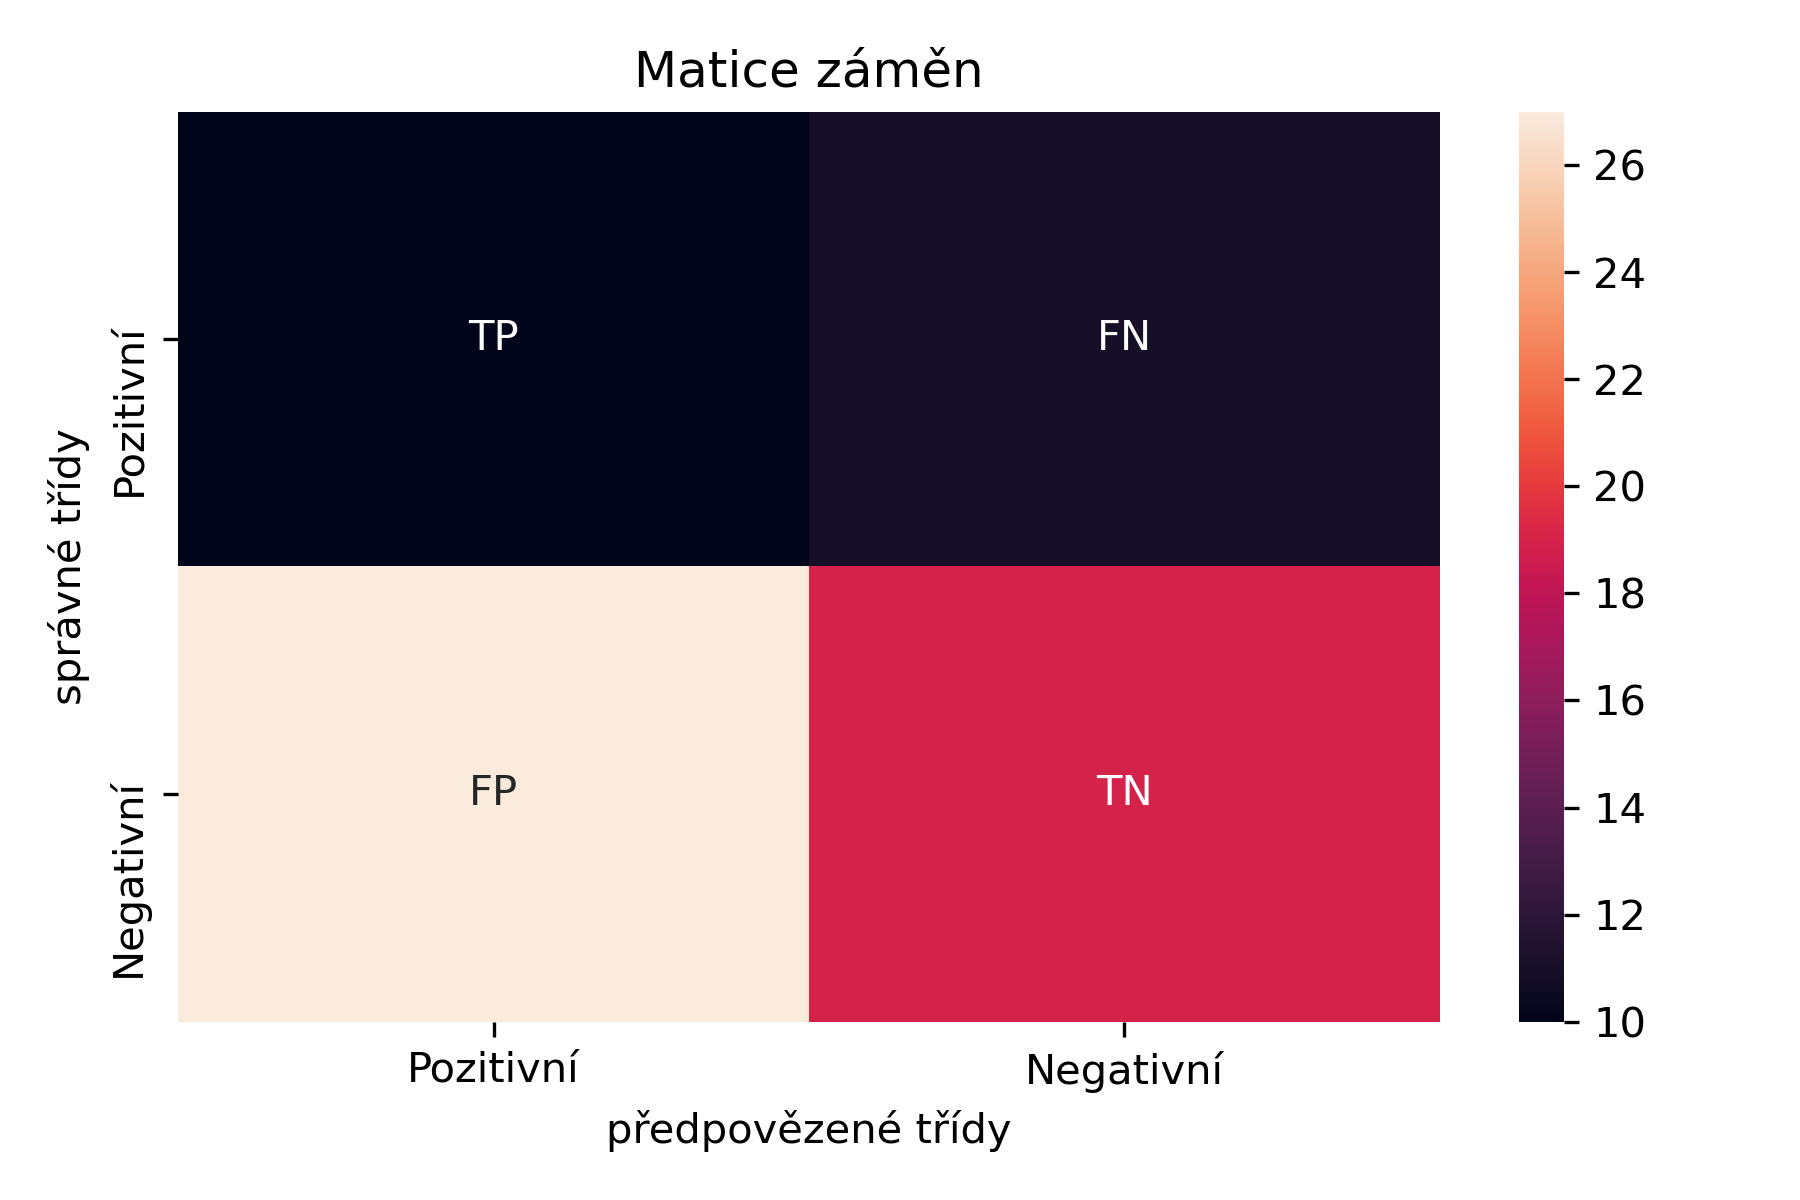
\includegraphics[scale=.7]{conf_matrix-example.png}}
\caption{Matice záměn pro dvě třídy}
\label{fig:conf_matrix-example}
\end{figure}
\FloatBarrier

kde TP a TN jsou počty správně klasifikovaných pozitivních a negativní tříd. FP a FN jsou množství nesprávně přiřazených pozitivních a negativních tříd.

\section{Vybrané koncepty}
\extend{zmínit, proč tyhle?}
% Vybrané koncepty
\subsection{Křížová entropie} % Grammer checked
Jako kriteriální funkci pro klasifikaci do více tříd lze použít křížovou entropii, která měří rozdíl mezi dvěma rozděleními pravděpodobnosti. Lze ji vyjádřit:

\begin{equation}
\label{eqn:cross_entropy}
l = -{\sum_{c}^{C}t_{c}\log p_{c}},
\end{equation}

kde $ l $ je výsledná ztráta. Index $ c $ odpovídá klasifikovaným třídám a $ C $ je počet tříd. Proměnná $ p $ značí vstupní pravděpodobnosti pro jednotlivé třídy, které dosahují hodnot od nuly do jedné. $ t $ zastupuje skutečné třídy. Minimalizací křížové entropie minimalizujeme rozdíl mezi pravděpodobnostním rozdělením trénovacích dat a pravděpodobnostním rozdělením předpovídaných hodnot~\cite{brownlee_2020}.

\subsection{ReLU} % Grammer checked
Usměrněná lineární aktivační funkce (ReLU) je aktivační funkce, jejíž výstupem je buď nula, pokud je vstup záporný nebo se hodnota vstupu nezmění, pokud je kladný. Lze ji vyjádřit:

\begin{equation}
\label{eqn:relu}
y = max(0, x),
\end{equation}

kde $ y $ jsou výstupní hodnoty. Proměnná $ x $ zastupuje vstupní hodnoty. Neuronové sítě používající tuto funkci se většinou učí rychleji a dosáhnou lepších výsledků. Výhodou této funkce je, že nepodléhá přesycení, kdy jsou velká čísla na příklad u funkce sigmoid změněna na jedna a velmi malá na nula. Důsledkem přesycení je, že jsou funkce jako sigmoid nebo tanh velice citlivé na hodnoty okolo jejich středu a méně na odlehlejší hodnoty. Následně se to projeví při trénovaní modelu, kdy může dojít k problému mizejícího gradientu u hlubších neuronových sítí~\cite{brownlee_2020_ReLU}. \extend{možná zmínit nevýhody? snadno exploding gradient?}

\subsection{Softmax} % Grammer checked
Softmax je funkce, která mění vektor čísel na vektor pravděpodobností, kde jsou pravděpodobnosti pro jednotlivé prvky úměrné velikosti všech prvků vektoru. Funkci lze vyjádřit vzorcem:

\begin{equation}
\label{eqn:softmax}
p_i = \frac{e^{s_i}}{\sum_{c}^{C}e^{s_c}},
\end{equation}

kde $ p_i $ je hodnota výstupní pravděpodobnosti. Proměnná $ s $ odpovídá skóre výstupní vrstvy neuronové sítě. Index $ i $ odpovídá třídě výstupní pravděpodobnosti a index $ c $ třídám skóre. Hodnota $ C $ je rovna počtu klasifikovaných tříd. Součet všech výsledných pravděpodobností je roven jedné. Funkce se používá při klasifikaci do více tříd a stojí na konci klasifikátoru. Každá výstupní pravděpodobnost odpovídá jednotlivé třídě datové sady~\cite{brownlee_2020_Softmax}.

\chapter{Vývoj balíčku pro rozpoznávání emocí} % Grammer checked
Byl vytvořen balíček s moduly pro rozpoznávání emocí. \note{asi bych to lépe uvedl, víc popsat, než začneš popisovat moduly}
Balíček je napsán v jazyku \texttt{\mbox{Python}}\footnote{https://www.python.org/} verze 3. Mezi vytvořené moduly patří: \texttt{\mbox{convertors}} pro převod dat, data pro práci s daty, \texttt{\mbox{classifiers}} na tvorbu klasifikátoru, \texttt{\mbox{files}} na práci se soubory, \texttt{\mbox{datasets}} k tvorbě datových sad, \texttt{\mbox{prepare}} pro přípravu datových sad a \texttt{\mbox{train}} sloužící k trénování modelu. Moduly jsou psány objektově. Byly použity knihovny a frameworky: \texttt{\mbox{PyTorch}}\footnote{https://pytorch.org} 1.6 pro tvorbu a trénování modelu, \texttt{\mbox{seaborn}} 0.11 a \texttt{\mbox{matplotlib}} 3.3 pro vytvoření grafů, \texttt{\mbox{logging}} 0.4 pro logování při trénování modelu, \texttt{\mbox{scikit-learn}} 0.23 pro rozdělení dat na datové sady, \texttt{\mbox{pandas}} 1.1 a \texttt{\mbox{numpy}} 1.18 pro ukládání a práci s daty, \texttt{\mbox{os}} a \texttt{\mbox{sys}} pro práci s operačním systémem, \texttt{\mbox{re}} pro parsování anotací, \texttt{\mbox{subprocess}} pro spouštění příkazů z příkazové řádky, \texttt{\mbox{PyHTK}}\footnote{https://github.com/danijel3/PyHTK} pro načítání souborů vytvořených pomocí sady nástrojů Hidden Markov Model Toolkit (\texttt{\mbox{HTK}})\footnote{https://htk.eng.cam.ac.uk}. \note{možná uvést následující podkapitoly, věnují se jednotlivým úlohám}

\section{Předzpracování dat} % Grammer checked
Data byla nejdříve předzpracována. Byl sjednocen jejich formát a data převedena na příznaky MFCC. Formát byl sjednocen pomocí nástroje Fast Forward MPEG (FFmpeg)\footnote{https://ffmpeg.org} přístupného z příkazové řádky. Nahrávky byly převedeny na vzorkovací frekvenci 16 kHz a byl zachován jeden zvukový kanál. Zvukové nahrávky byly převedeny pomocí příkazu na obrázku \mbox{\ref{fig:ffmpeg}}.

\begin{figure}[htbp]
\centerline{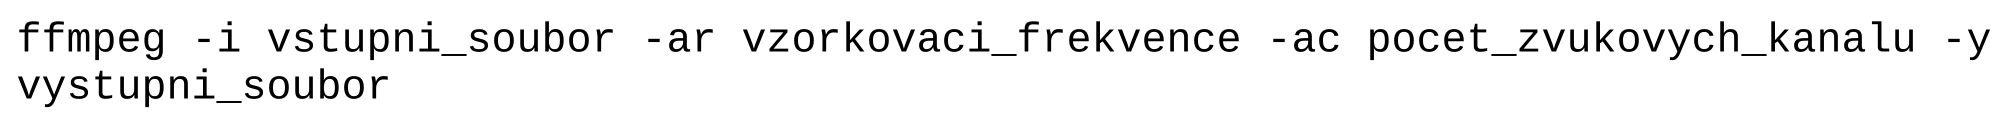
\includegraphics[width=\textwidth,height=\textheight,keepaspectratio]{ffmpeg_command.png}}
\caption{Příkaz FFmpeg}
\label{fig:ffmpeg}
\end{figure}
\FloatBarrier

Dále byly z nahrávek extrahovány příznaky MFCC. K extrakci byla použita sada nástrojů HTK. Pro extrakci byl použit konfigurační soubor (viz obr. \mbox{\ref{fig:htk_config})}.

\begin{figure}[htbp]
\centerline{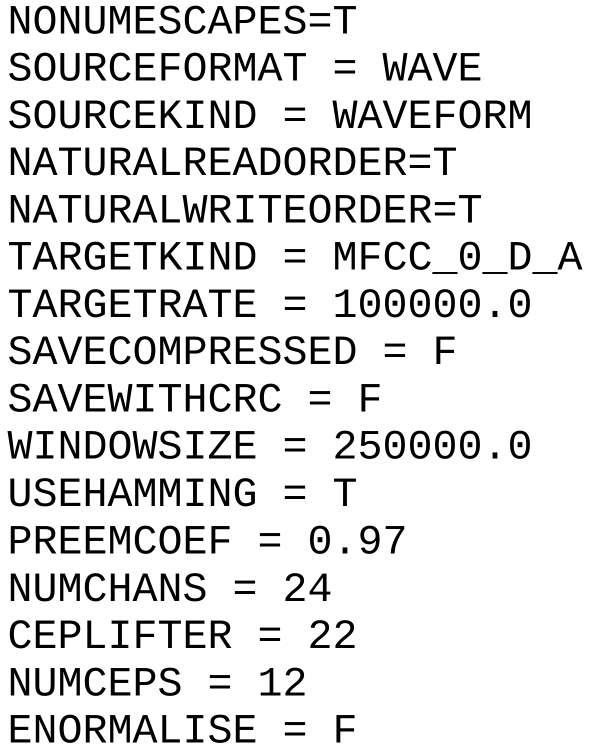
\includegraphics[scale=.2,keepaspectratio]{htk_config.png}}
\caption{HTK konfigurační soubor}
\label{fig:htk_config}
\end{figure}
\FloatBarrier

MFCC formát byl zvolen jako MFCC\_0\_D\_A, jehož cílem bylo získat nulté, delta a akcelerační koeficienty. Dále lze vyčíst, že pro okénkování byla použita Hammingova okénkovací funkce a velikost okénka byla nastavena na 25 ms. Extrakce byla uskutečněna pomocí příkazu \texttt{\mbox{HCOPY}} na obrázku \mbox{\ref{fig:htk}}. Pro každý rámec nahrávky bylo získáno 39 příznaků.

\begin{figure}[htbp]
\centerline{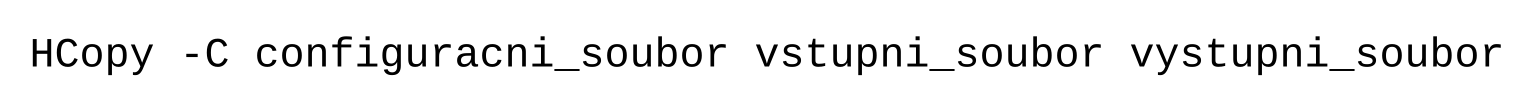
\includegraphics[width=\textwidth,height=\textheight,keepaspectratio]{htk_command.png}}
\caption{HCopy příkaz}
\label{fig:htk}
\end{figure}
\FloatBarrier

Třídy pro převod byly implementovány v modulu \texttt{\mbox{convertors}}. Byla vytvořena základní třída \texttt{\mbox{Convertor}}, z které konkrétní převaděče dědí. Pro sjednocení formátu byla vytvořena třída \texttt{\mbox{AudioFormatConverter}} a třída \texttt{\mbox{MFCCConverter}} pro převod na příznaky MFCC. Vztahy mezi převaděči jsou znázorněny na UML diagramu \mbox{\ref{fig:convertor}}.

\begin{figure}[ht]
\centerline{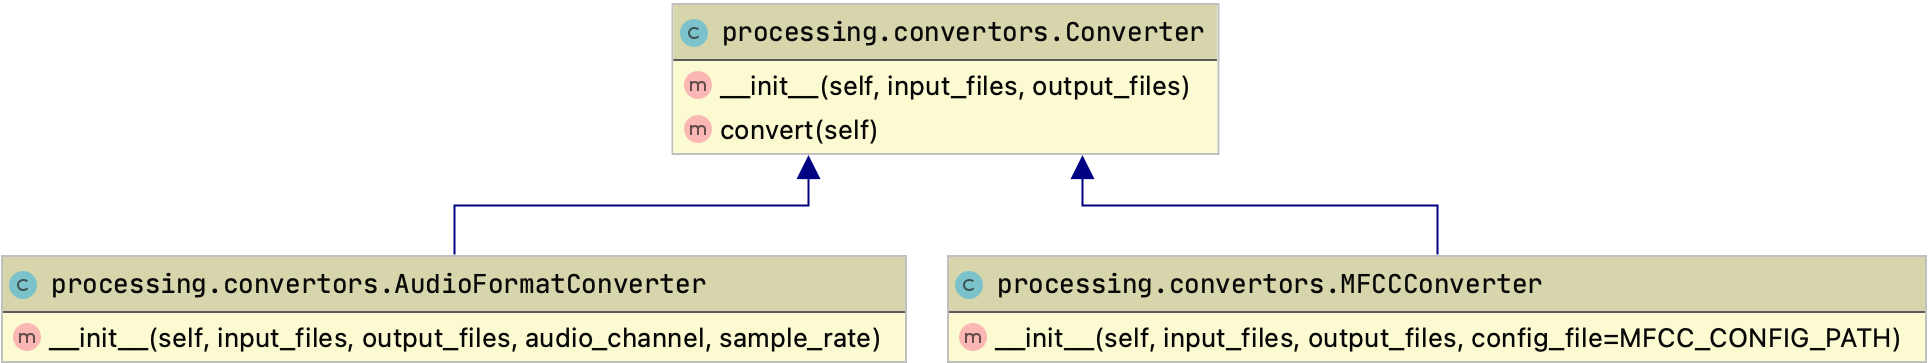
\includegraphics[width=\textwidth,height=\textheight,keepaspectratio]{convertors.png}}
\caption{Třídy Converter}
\label{fig:convertor}
\end{figure}
\FloatBarrier

\section{Příprava datových sad pro trénování} % Grammer checked
Pro načítání dat byla vytvořena třída \texttt{\mbox{Dataset}} v modulu \texttt{\mbox{data}}. Hlavními úkoly této třídy bylo načíst data a z anotací získat třídy emocí. Třída \texttt{\mbox{Dataset}} dědí od třídy \texttt{\mbox{Directory}} z modulu \texttt{\mbox{files}}, která umožňuje získat cesty k souborům ve složce. Vztah mezi třídami je znázorněn na diagramu \mbox{\ref{fig:datasets}}.

\begin{figure}[h!]
\centerline{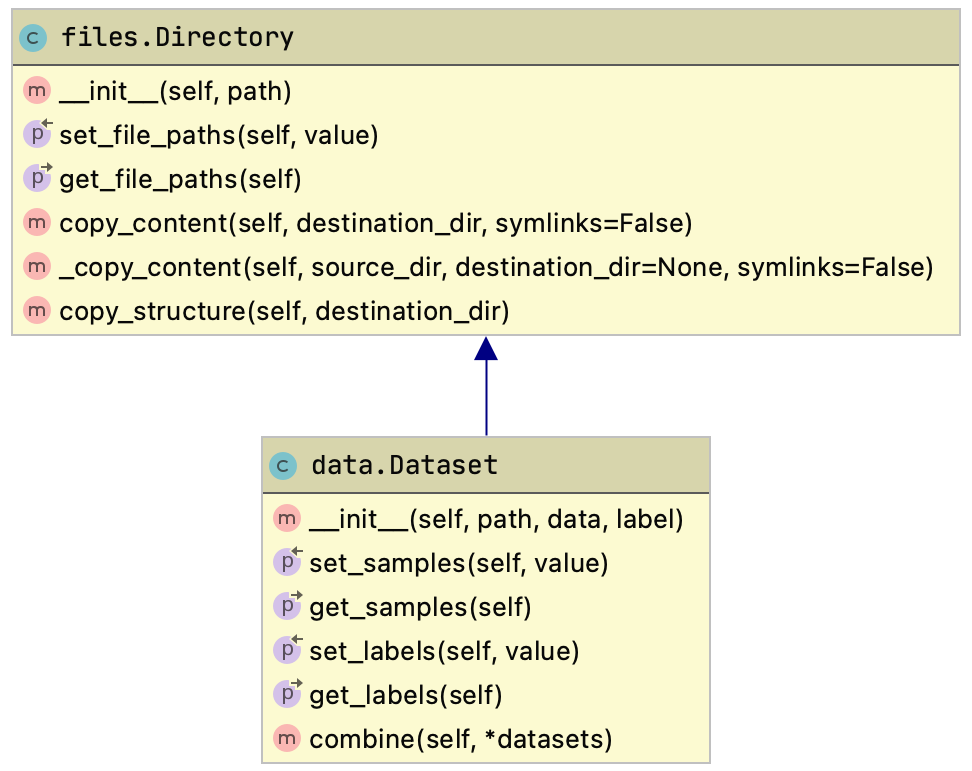
\includegraphics[scale=.25,keepaspectratio]{data-dataset.png}}
\caption{Třída Dataset}
\label{fig:datasets}
\end{figure}
\FloatBarrier

Třída \texttt{\mbox{Dataset}} má navíc atributy \texttt{\mbox{samples}} pro uložení načtených vzorků a \texttt{\mbox{labels}} pro uložení anotací pro vzorky. Při vytváření objektu třídy \texttt{\mbox{Dataset}} jsou předávány objekty třídy \texttt{\mbox{Data}} a \texttt{\mbox{Label}}. Objekt třídy \texttt{\mbox{Data}} načte na základě cesty k souboru vzorek a \texttt{\mbox{Label}} z anotace získá informace potřebné k vytvoření anotace pro vzorek. Jelikož jsou datové sady odlišně značeny, byly vytvořeny třídy dědící od třídy \texttt{\mbox{UnifiedLabel}} (viz obr. \mbox{\ref{fig:label}}), které navíc anotace pro vzorky převedly na stejné značení.

\begin{figure}[ht]
\centerline{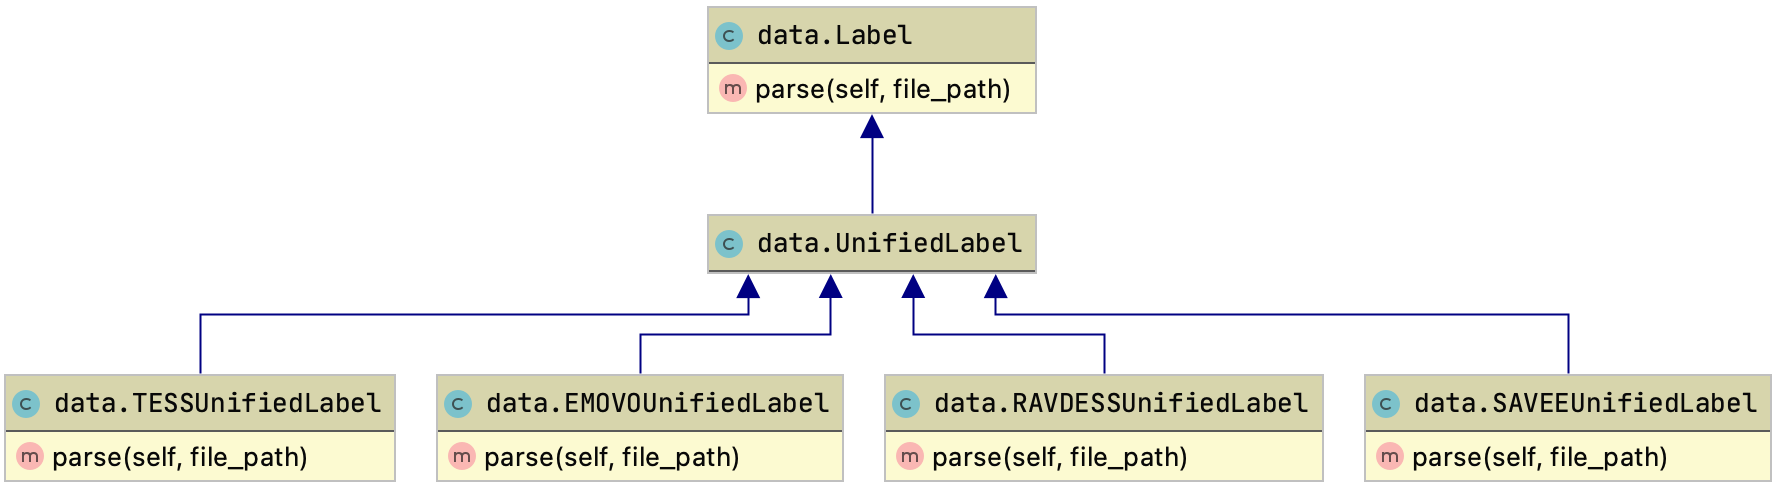
\includegraphics[scale=.25,keepaspectratio]{data-label.png}}
\caption{Třídy Label}
\label{fig:label}
\end{figure}
\FloatBarrier

Z třídy \texttt{\mbox{Data}} (viz obr. \mbox{\ref{fig:data}}) dědí třída \texttt{\mbox{MFCCData}} umožňující načtení příznaků MFCC a \texttt{\mbox{WAVData}} zprostředkovávající načtení nahrávek ze souboru typu WAV. \texttt{\mbox{MFCCData}} používá třídu \texttt{\mbox{HTKFile}} z balíčku \texttt{\mbox{PyHTK}} pro načtení příznaků.

\begin{figure}[ht]
\centerline{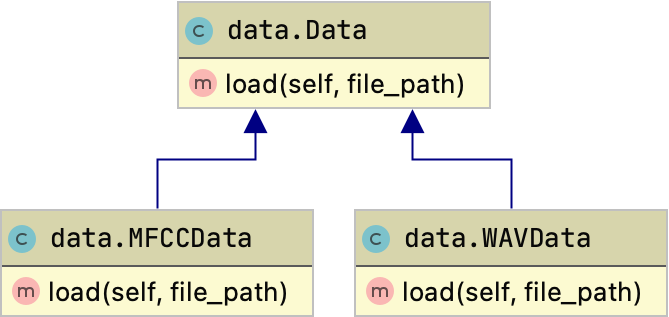
\includegraphics[scale=.25,keepaspectratio]{data-data.png}}
\caption{Třídy Data}
\label{fig:data}
\end{figure}
\FloatBarrier

Dále byla data rozdělena do trénovacích, validačních a testovacích sad. Pro rozdělení byla použita třída \texttt{\mbox{Preparer}} (viz obr. \ref{fig:preparer}) z modulu \texttt{\mbox{prepare}}. Data byla nejdříve načtena pomocí objektů třídy \texttt{\mbox{Dataset}}. Umožňuje libovolný výběr datových sad a jejich sloučení. Data získaná z objektu \texttt{\mbox{Dataset}} mohla být rozdělena do trénovacího, testovacího a validačního setu. Rozdělení probíhalo rovnoměrně pomocí funkce \texttt{\mbox{train\_test\_split}} z modulu \texttt{\mbox{sklearn.model\_selection}} a vzorky byly rozděleny po celých nahrávkách. Při rozdělování na sady byla zvolena možnost \texttt{\mbox{stratify}}, která rozdělila vzorky rovnoměrně do vzniklých sad podle anotací.

\begin{figure}[ht]
\centerline{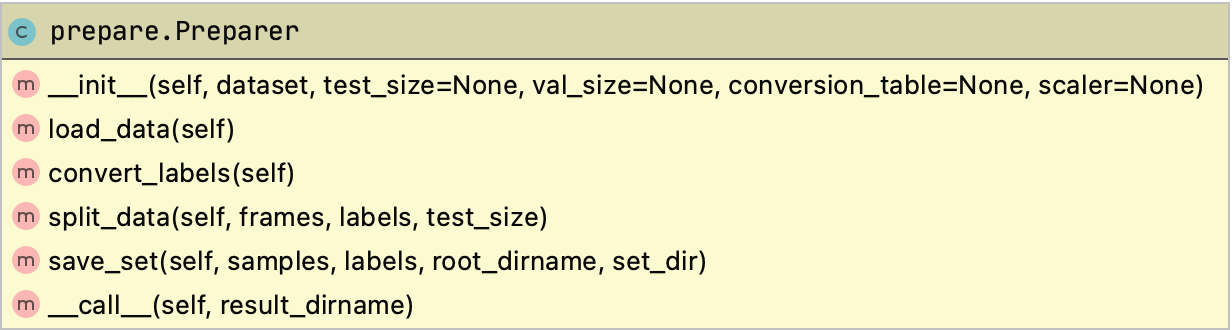
\includegraphics[scale=.25,keepaspectratio]{prepare.png}}
\caption{Třída Preparer}
\label{fig:preparer}
\end{figure}
\FloatBarrier

Jako poslední byly sady uloženy do složky. Každé sadě byla přiřazena vlastní složka, která obsahovala soubory labels.npy, samples.npy a info.txt. V souboru info.txt byly uloženy informace pro načítání datové sady. Struktura složky je znázorněna na obrázku \mbox{\ref{fig:file_structure}}. 

\begin{figure}[ht]
\centerline{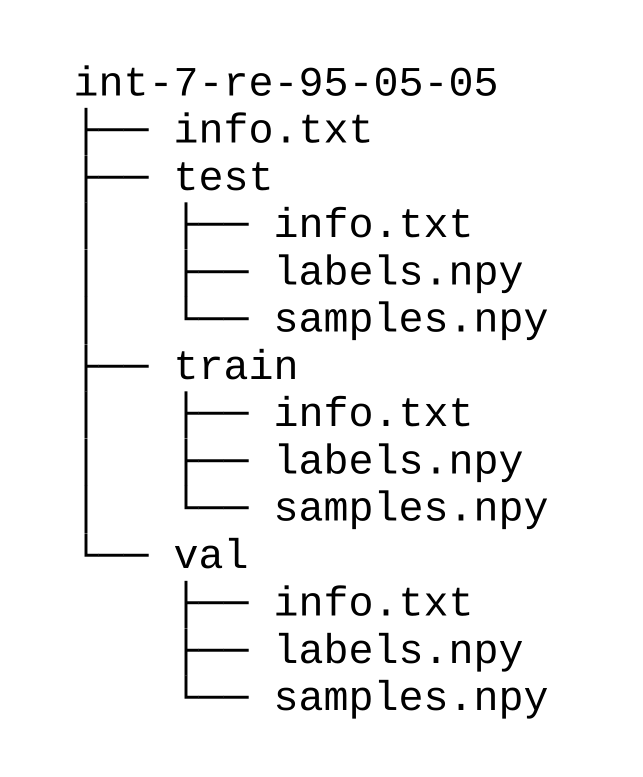
\includegraphics[scale=.22]{dataset_file_structure.png}}
\caption{Souborová struktura uložené datové sady}
\label{fig:file_structure}
\end{figure}
\FloatBarrier

Pro ukládání a načítání informací ze souborů info.txt byly vytvořeny třídy \texttt{\mbox{DatasetInfoFile}} (viz obr. \mbox{\ref{fig:info_files}}) a \texttt{\mbox{SetInfoFile}}. V souboru třídy \texttt{\mbox{DatasetInfoFile}} byly uloženy údaje o počtu příznaků, počtu tříd a počtu vzorků datové sady. Do \texttt{\mbox{SetInfoFile}} byly ukládány počty vzorků, délky vzorků a názvy souborů se vzorky a anotacemi. Data pro rozpoznávání byla uložena ve dvourozměrném poli \texttt{\mbox{numpy}}.

\begin{figure}[ht]
\centerline{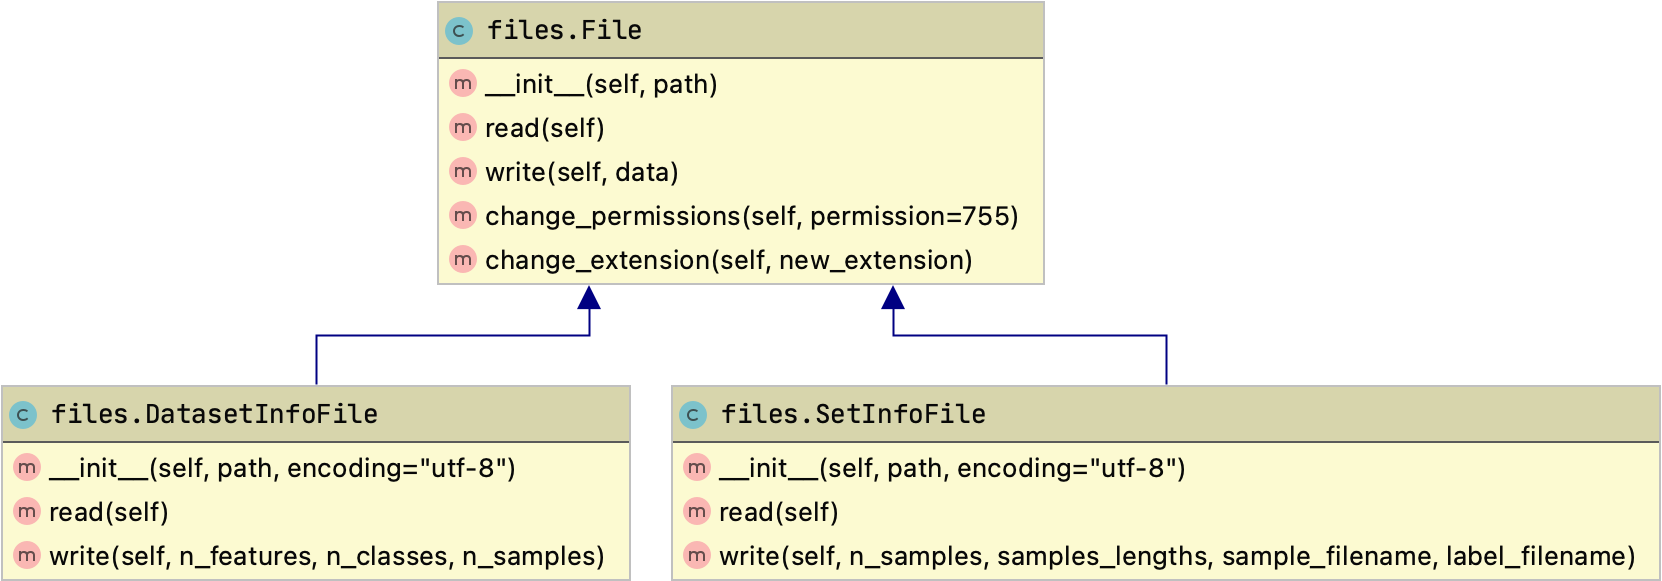
\includegraphics[scale=.25]{files-info.png}}
\caption{Třídy InfoFile}
\label{fig:info_files}
\end{figure}
\FloatBarrier

\section{Načítání dat} % Grammer checked
Pro načítání uložených datových sad byla vytvořena třída \texttt{\mbox{NumpyDataset}}, která dědí od třídy \texttt{\mbox{Dataset}} z balíčku \texttt{\mbox{torch.utils.data}}. Při vytvoření je objektu třídy přidělena cesta k datové sadě. Z textového souboru info.txt se přečtou informace potřebné k načtení dat. Mezi důležité parametry, které objekt \texttt{\mbox{NumpyDataset}} při svém vytvoření přebírá, patří velikosti pravého a levého okolí vzorku. Při načtení vzorků ze souboru samples.npy jsou ke vzorkům na začátku a na konci přiřazeny okraje, které mají velikosti pravého a levého okolí. Okraje jsou vytvořeny z kopií krajních vzorků a slouží pro zjednodušení výběrů vzorků. Vzorky jsou uloženy popořadě po jednotlivých nahrávkách. Objekt si ukládá indexy začátku a konce nahrávek. Načtené anotace z připravené datové sady odpovídají jednotlivým nahrávkám, proto jsou anotace roztaženy tak, aby odpovídaly délce vzorků nahrávky. Uložení vzorků v objektu \texttt{\mbox{NumpyDataset}} je znázorněno na diagramu \mbox{\ref{fig:data_arrangement}}.

\begin{figure}[htbp]
\centerline{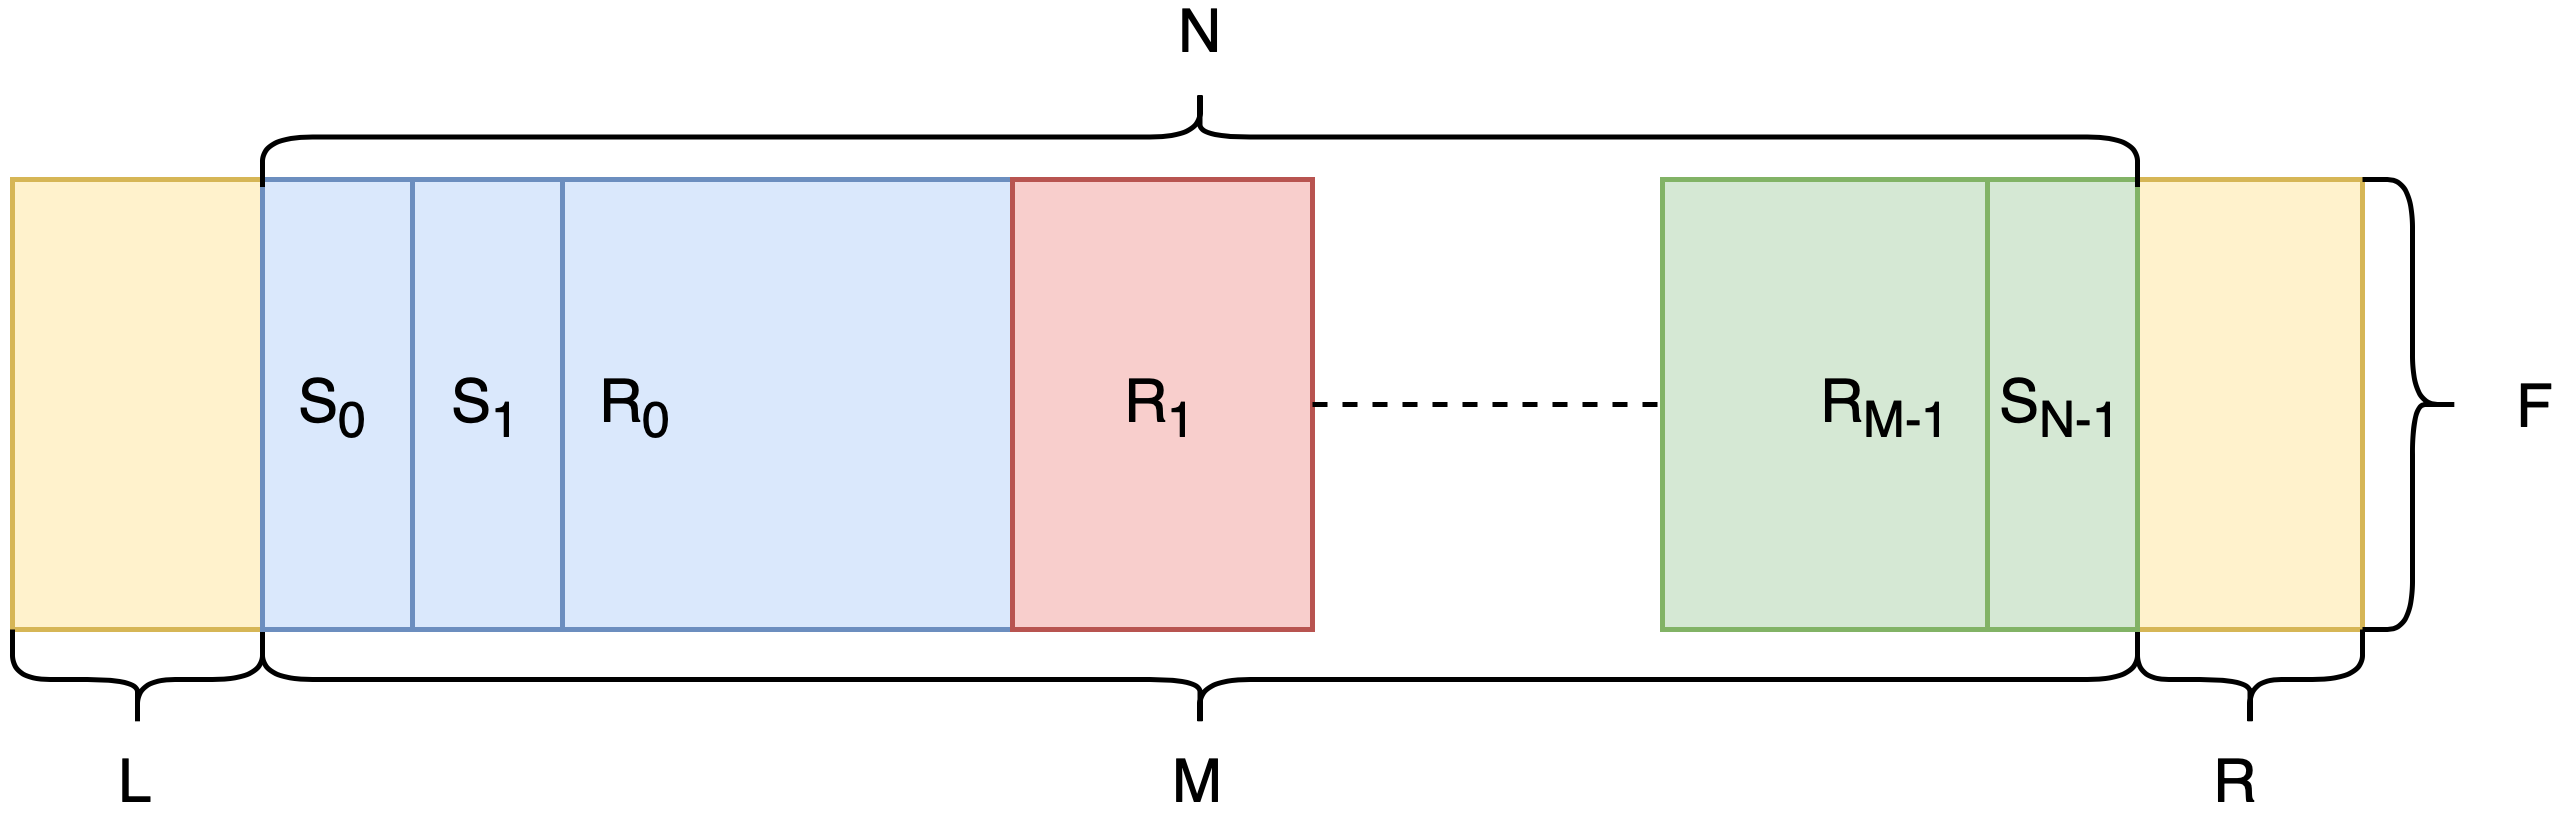
\includegraphics[scale=.125]{dataset_arrangement.png}}
\caption{Uspořádání dat v NumpyDatasetu}
\label{fig:data_arrangement}
\end{figure}
\FloatBarrier

Písmenem $ S $ jsou označeny jednotlivé vzorky. $ R $ označuje jednotlivé nahrávky, které mohou mít různou délku. Písmeno $ N $ udává počet vzorků a $ M $ počet uložených nahrávek. $ L $ a $ R $ značí velikost pravého a levého okraje. Písmeno $ F $ odpovídá počtu příznaků pro jeden vzorek.

Z třídy \texttt{\mbox{NumpyDataset}} dědí třídy \texttt{\mbox{NumpyFrameDataset}} a \texttt{\mbox{NumpySampleDataset}} (viz obr. \mbox{\ref{fig:numpy_dataset}}), které se liší v implementaci metod \texttt{\_\_len\_\_} a \texttt{\_\_getitem\_\_}. Metoda \texttt{\_\_len\_\_} při zavolání vrací délku datové sady, která u třídy \texttt{\mbox{NumpyFrameDataset}} odpovídá počtu vzorků a u třídy \texttt{\mbox{NumpySampleDataset}} odpovídá počtu nahrávek. Metoda \texttt{\_\_getitem\_\_} vrací jeden prvek z \texttt{\mbox{Dataset}}, u třídy \mbox{NumpySampleDataset} vrací metoda jeden vzorek a třídy \texttt{\mbox{NumpyRecordingDataset}} vrací jednu nahrávku. Třída \texttt{\mbox{NumpyDataset}} je tímto způsobem rozdělena. Důvodem pro rozdělení je, že při načítání dat pro validaci můžeme pomocí třídy \texttt{\mbox{NumpyRecordingDataset}} spočítat přesnost na celou nahrávku. Naopak při trénování je potřeba načítat vzorky po dávkách, které mají fixní délku na rozdíl od nahrávek, u kterých se délka mění. Vzorky se při trénování často míchají, a to je také důvod, proč je lepší mít třídu rozdělenou.

\begin{figure}[ht]
\centerline{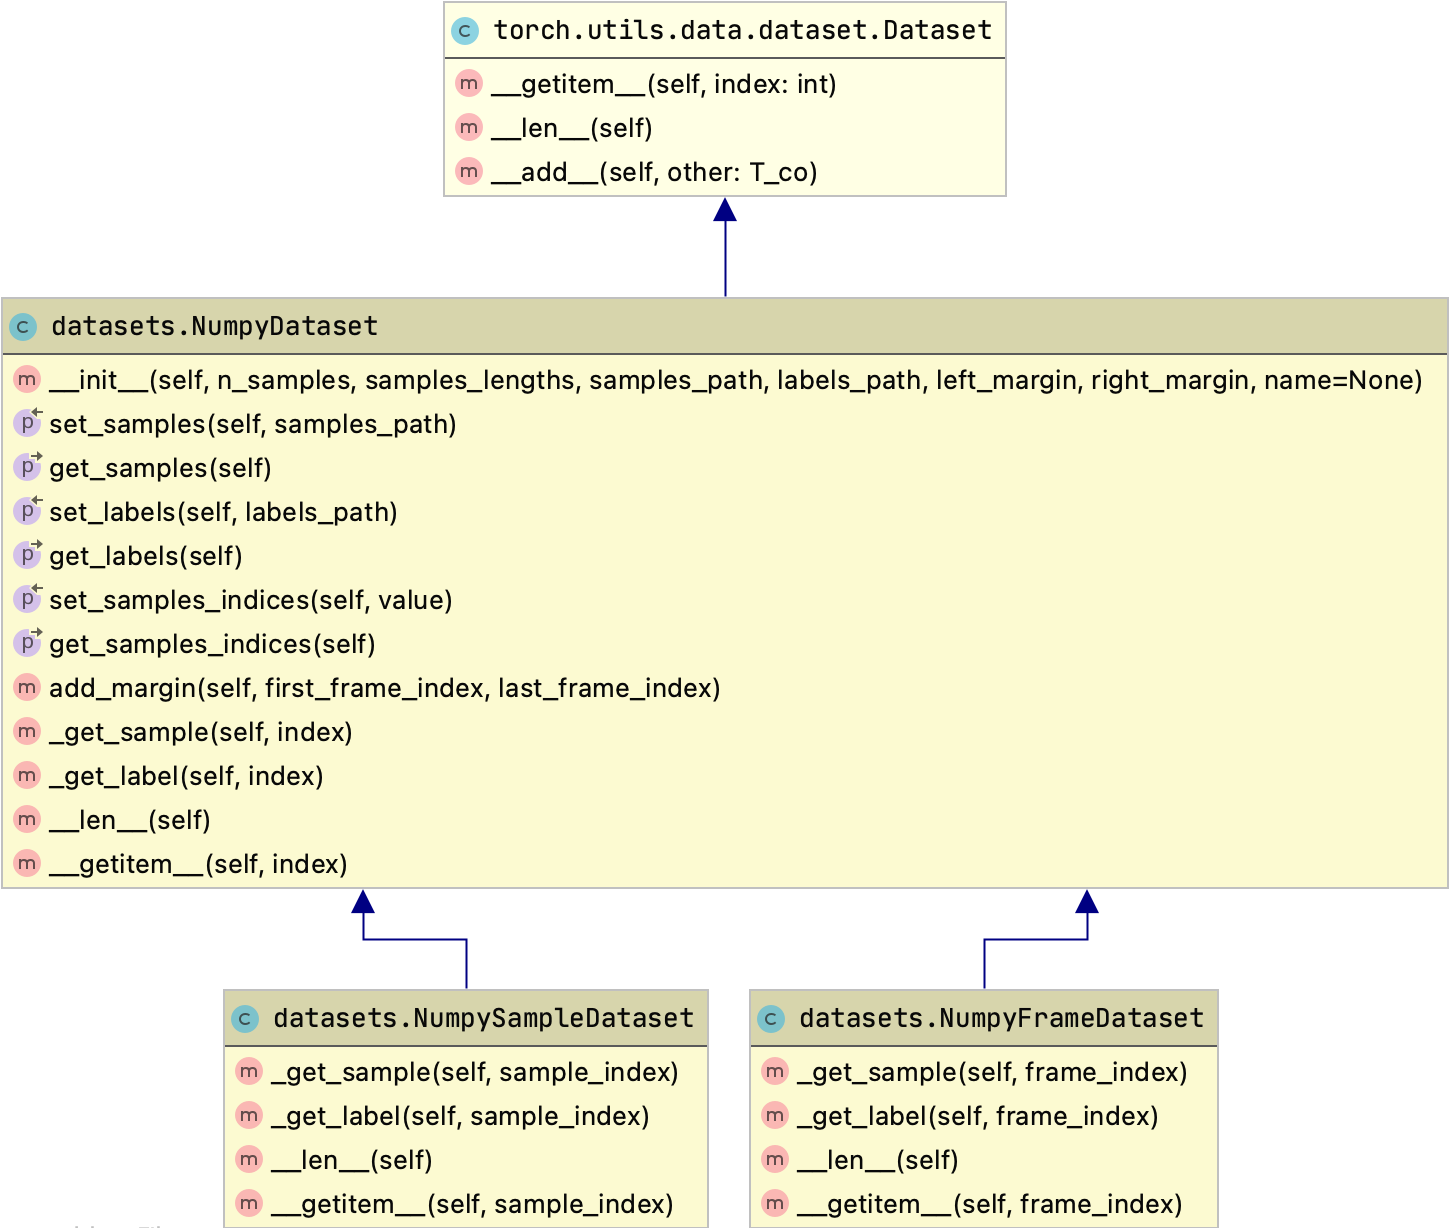
\includegraphics[scale=.185]{datasets.png}}
\caption{Třídy NumpyDataset}
\label{fig:numpy_dataset}
\end{figure}
\FloatBarrier

Ke vzorkům jsou při výběru přidávány vzorky z okolí pro větší zachycení kontextu nahrávky. Počet vzorků z okolí je načítán na základě velikosti pravého a levého okraje. Vybrané vzorky jsou před vrácením zploštěny. Proces výběru vzorku je znázorněn na obrázku \mbox{\ref{fig:sample_selection}}. \change{mrkni se, jak se píší odkazy na obrázky}

\begin{figure}[ht]
\centerline{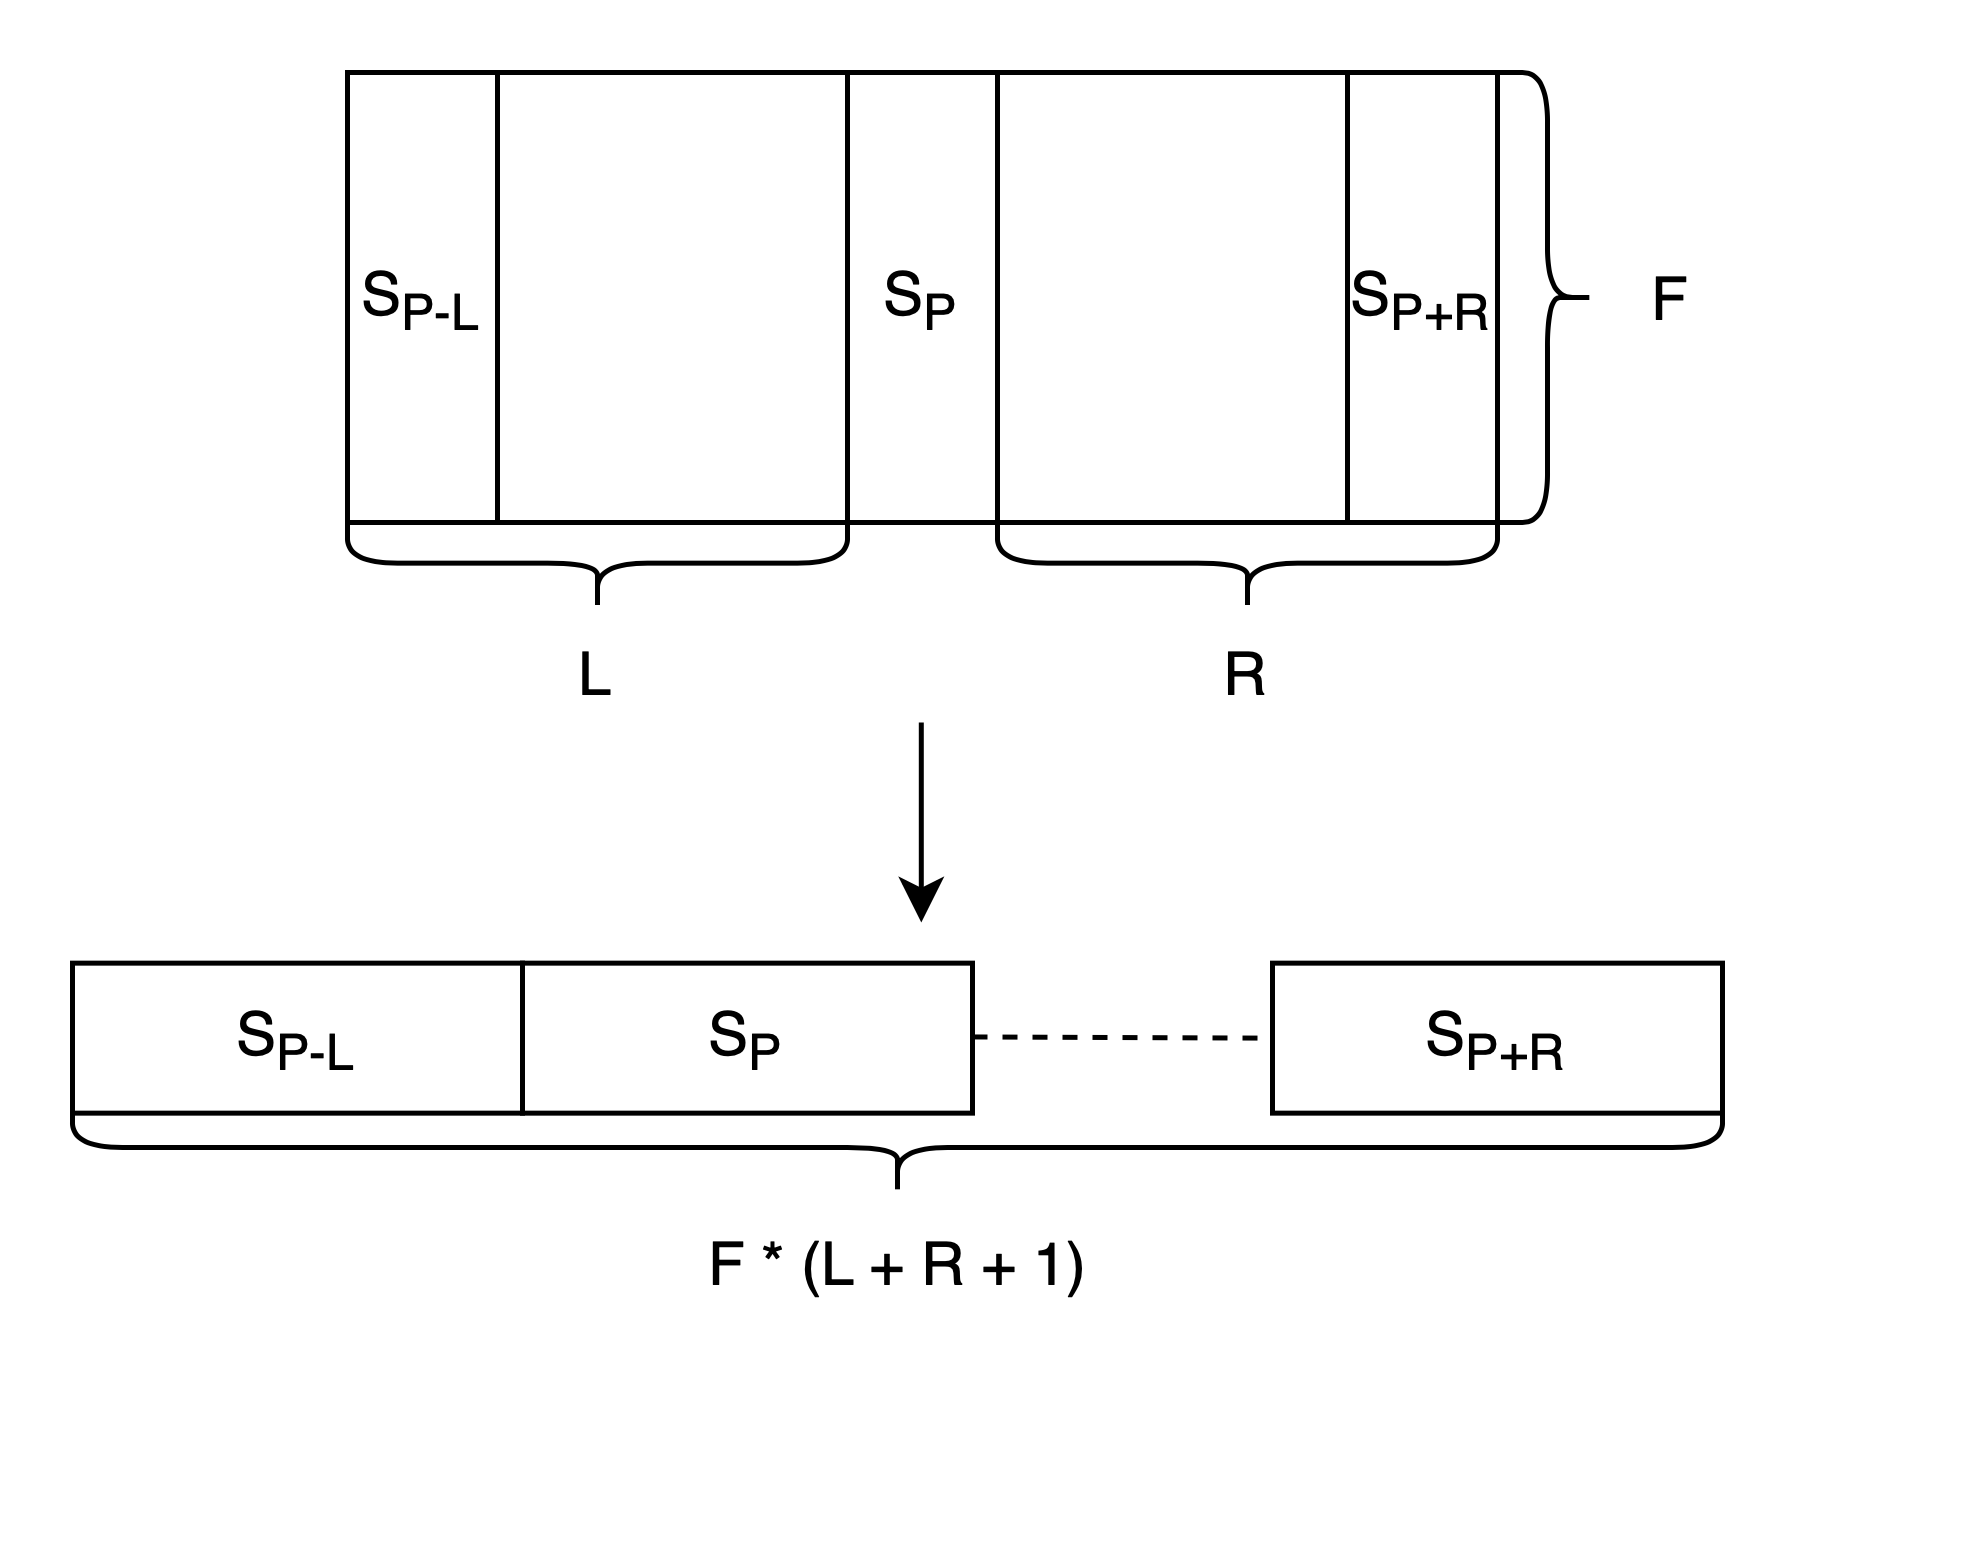
\includegraphics[scale=.22]{sample_selection.png}}
\caption{Výběr vzorku}
\label{fig:sample_selection}
\end{figure}
\FloatBarrier

Vybraný vzorek má označení $ S_{P} $ a krajní vzorky mají označení $ S_{P-L} $ a $ S_{P+R} $. Písmeno $ F $ označuje počet příznaků pro jeden vzorek. Značky $ L $ a $ P $ odpovídají délkám levého a pravého okraje. Výsledný zploštělý obrázek má délku odpovídající $ F \cdot (L + R + 1) $.

\section{Tvorba neuronové sítě} % Grammer checked
Pomocí frameworku \texttt{\mbox{PyTorch}} byl vytvořen model \texttt{\mbox{FeedForwardNet}} pomocí dědění z třídy \texttt{\mbox{Module}} z modulu \texttt{\mbox{torch.nn}}. V konstruktoru třídy \texttt{\mbox{FeedForwardNet}} byly poskládány jednotlivé vrsty neuronové sítě a byly uloženy do objektu \texttt{\mbox{ModuleList}} z modulu \texttt{\mbox{torch.nn}}. Dále byl pomocí metody \texttt{\mbox{forward}} implementován dopředný průchod.

\subsection{Trénování} % Grammer checked
V modulu \texttt{\mbox{train}} byla vytvořena třída \texttt{\mbox{Trainer}} (viz obr. \mbox{\ref{fig:trainer}}), jejíž úkolem je trénování modelu. Hlavní parametr předaný při vytváření instance třídy je \texttt{\mbox{model}}. Dále jsou předány trénovací, testovací a validační sady. Pro trénování modelu jsou důležité parametry \texttt{\mbox{optimizer}} k úpravě parametrů a kriteriální funkce pro získání ztráty. Parametr \texttt{\mbox{device}} umožňuje zvolit zařízení, na kterém bude trénování probíhat. Jako poslední je předán objekt typu \texttt{\mbox{Stats}} (viz obr. \mbox{\ref{fig:stats}}), do kterého se ukládají statistiky získané při trénování modelu. 

\begin{figure}[ht]
\centerline{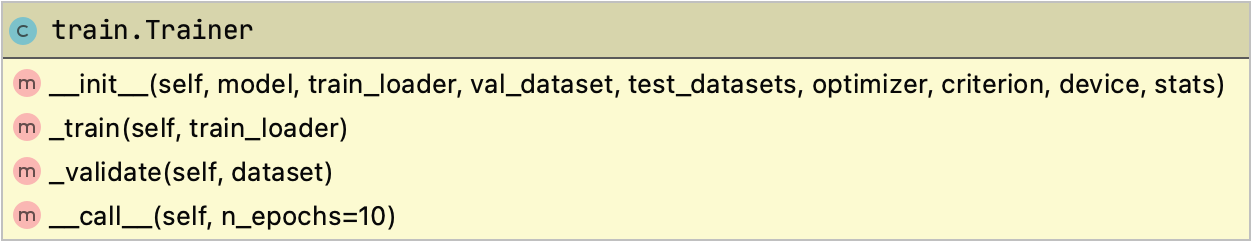
\includegraphics[scale=.3]{train-trainer.png}}
\caption{Třída Trainer}
\label{fig:trainer}
\end{figure}
\FloatBarrier

\begin{figure}[ht]
\centerline{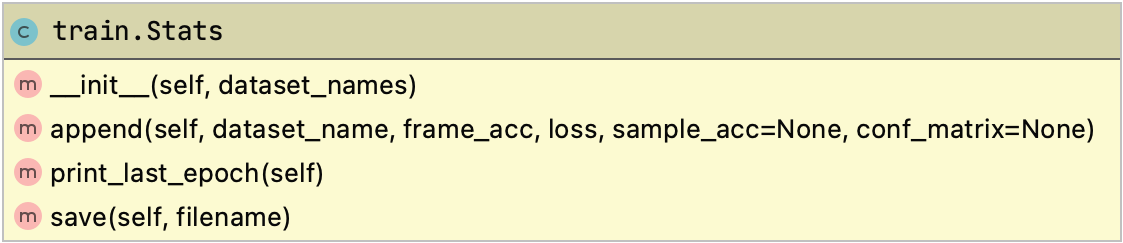
\includegraphics[scale=.33]{train-stats.png}}
\caption{Třída Stats}
\label{fig:stats}
\end{figure}
\FloatBarrier

Trénování je zahájeno zavoláním objektu třídy \texttt{\mbox{Trainer}}, kdy je předán počet trénovacích epoch. Každou epochu jsou do objektu třídy \texttt{\mbox{Stats}} ukládány statistiky trénování, mezi které patří přesnost na jeden vzorek, přesnost na jednu nahrávku, ztráta modelu a matice záměn. Zároveň jsou vybrané statistiky vypisovány v přehledném výpisu (viz obr. \mbox{\ref{fig:print}}) do konzole. K výpisu je používán objekt třídy \texttt{\mbox{StatsPrinter}} (viz obr. \mbox{\ref{fig:printer}}).

\begin{figure}[ht]
\centerline{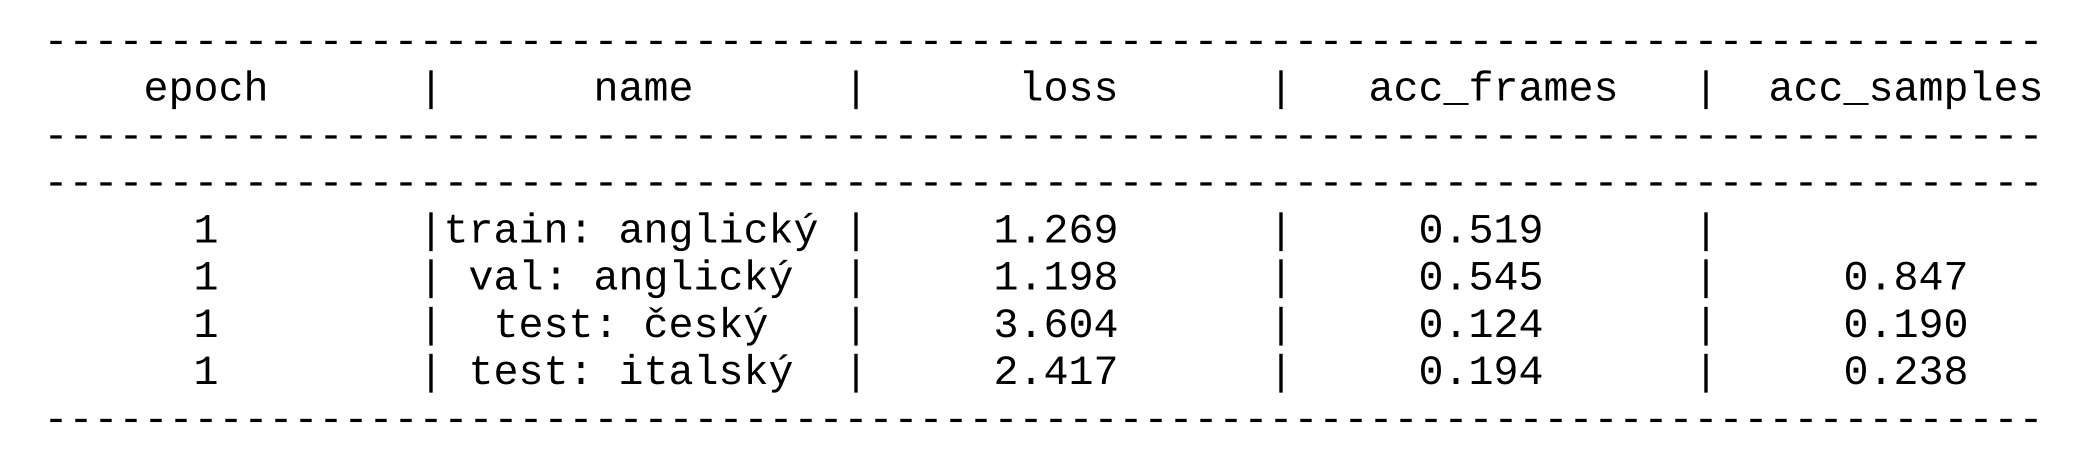
\includegraphics[scale=.215]{train_log.png}}
\caption{Přehledný výpis průběhu trénování}
\label{fig:print}
\end{figure}
\FloatBarrier

\begin{figure}[ht]
\centerline{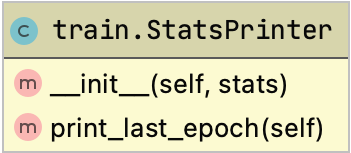
\includegraphics[scale=.32]{train-stats_printer.png}}
\caption{Třída StatsPrinter}
\label{fig:printer}
\end{figure}
\FloatBarrier

Po ukončení trénování lze model uložit do souboru s koncovkou .pt. Statistiky trénování lze uložit do souboru CSV. Ze statistik lze pomocí třídy \texttt{\mbox{Results}} (viz obr. \mbox{\ref{fig:results}}) získat grafy průběhu trénování. Pomocí funkce \texttt{\mbox{plot}} z knihovny \texttt{\mbox{matplolib}} jsou vykresleny grafy průběhu trénování pro přesnosti a ztrátu. Dále jsou vytvořeny pomocí funkce \texttt{\mbox{heatmap}} z knihovny \texttt{\mbox{seaborn}} grafy matice záměn. Grafy lze zobrazit a uložit jako obrázky typu PNG.

\begin{figure}[ht]
\centerline{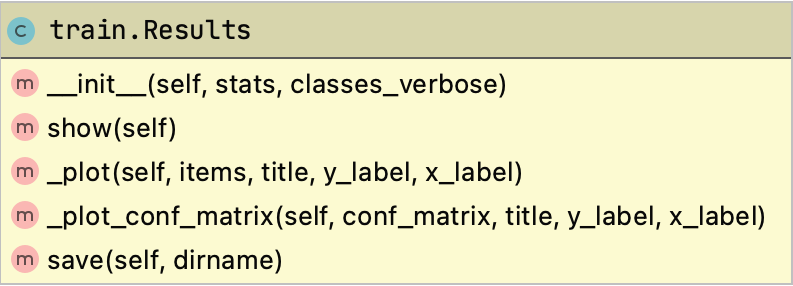
\includegraphics[scale=.3]{train-results.png}}
\caption{Třída Results}
\label{fig:results}
\end{figure}
\FloatBarrier

\chapter{Výběr datových sad} % Grammer checked
\note{nebylo by to lepší až v experimentech?}
Hlavním kritériem při výběru byla dostupnost datové sady, proto byly vybrány sady bezplatné a dostupné pro vědecké účely. Byly vybrány datové sady především anglické: RAVDESS, TESS a SAVEE a jedna italská: EMOVO. Datové sady mají společných sedm emocí, mezi které patří emoce: neutrální stav, hněv, strach, smutek, spokojenost, odpor a překvapení. Jelikož měla datová sada RAVDESS osm emocí, byla emoce klidu přidána mezi neutrální stav. Informace o datových sadách byly shrnuty v tabulce \mbox{\ref{tab:overview}}.

\begin{table}[ht]
\centering
\caption{Přehled vybraných datových sad}
\resizebox{\textwidth}{!}{\begin{tabular}{|c|c|c|c|c|c|c|}
  \hline
 \thead{Název} & \thead{Jazyk} & \thead{Počet tříd} & \thead{Počet mluvčích} & \thead{Pohlaví mluvčích} & \thead{Počet promluv} & \thead{Celková délka (hodiny)} \\
  \hline
    RAVDESS & angličtina & 8 & 24 & obě & 1440 & 1.5 \\
    SAVEE   & angličtina & 7 & 4  & muži  & 480  & 0.5 \\
    TESS    & angličtina & 7 & 2  & ženy  & 2800 & 1.6 \\
    EMOVO   & italština  & 7 & 6  & obě & 588  & 0.5 \\
   \hline
\end{tabular}}
\label{tab:overview}
\end{table}
\FloatBarrier

Celkem tedy byly získány čtyři datové sady o dvou jazycích se zastoupením sedmi emocemi. Dohromady vzniklá datová sada má celkem přibližnou dobu trvání čtyři hodiny.

\note{Měněna jedna věc dodat}
\chapter{Experimenty} % Grammer checked
\extend{více uvést, cílem je taky zlepšít výsledky, ne?}
Bylo provedeno několik experimentů pro vyladění hyperparametrů modelu s cílem zlepšení výsledků. Jako první byl proveden výchozí experiment, který sloužil k porovnání s dalšími experimenty. Trénovací, validační a testovací sady byly vytvořeny ze všech vybraných anglických datových sad a italské datové sady. Z každé vybrané datové sady byly rovnoměrně rozděleny vzorky podle tříd do sad v poměru \mbox{80 \%} nahrávek přišlo do trénovací sady, \mbox{10 \%} do sady testovací a 10 \% do sady validační.

\section{Výchozí model}
Jako první byl vytvořen výchozí model, který slouží k porovnání výkonu mezi modely. Pro získání ztráty modelu byla jako kriteriální funkce zvolena křížová entropie. Byl zvolen algoritmus Adaptive Momentum (Adam) pro optimalizaci modelu a míra učení byla nastavena na hodnotu 0,001. Model se skládal ze tří skrytých lineárních vrstev o šířce 128 neuronů. Ve skryté vrstvě byla použita aktivační funkce ReLU. Model byl trénován po dobu deseti epoch s velikostí jedné dávky 256 vzorků. Velikost pravého a levého okolí byla rovna 25 vzorkům. Bylo klasifikováno sedm emocí: hněv, znechucení, strach, radost, překvapení, smutek a neutrální stav.

Během trénování modelu přesnost pro vzorky na trénovací sadě stoupala až k hodně \mbox{83,1 \%} a na trénovací sadě kolísala kolem \mbox{59 \%}. \note{hodně?} Ztráta modelu na trénovací sadě postupně klesala. Model měl tendenci se přeučovat na trénovací sadě, dosvědčovalo tomu stoupání ztráty na validační sadě. Přesnost pro nahrávky dosáhla kolem \mbox{87 \%} na validační a testovací sadě. Úspěch dokládá i rozložení předpovědí v matici záměn pro validační sadu (viz obr. \mbox{\ref{fig:conf_matrix-val-baseline}}), kde je většina předpovědí umístěna na hlavní diagonále.

\begin{figure}[!htbp]
\centerline{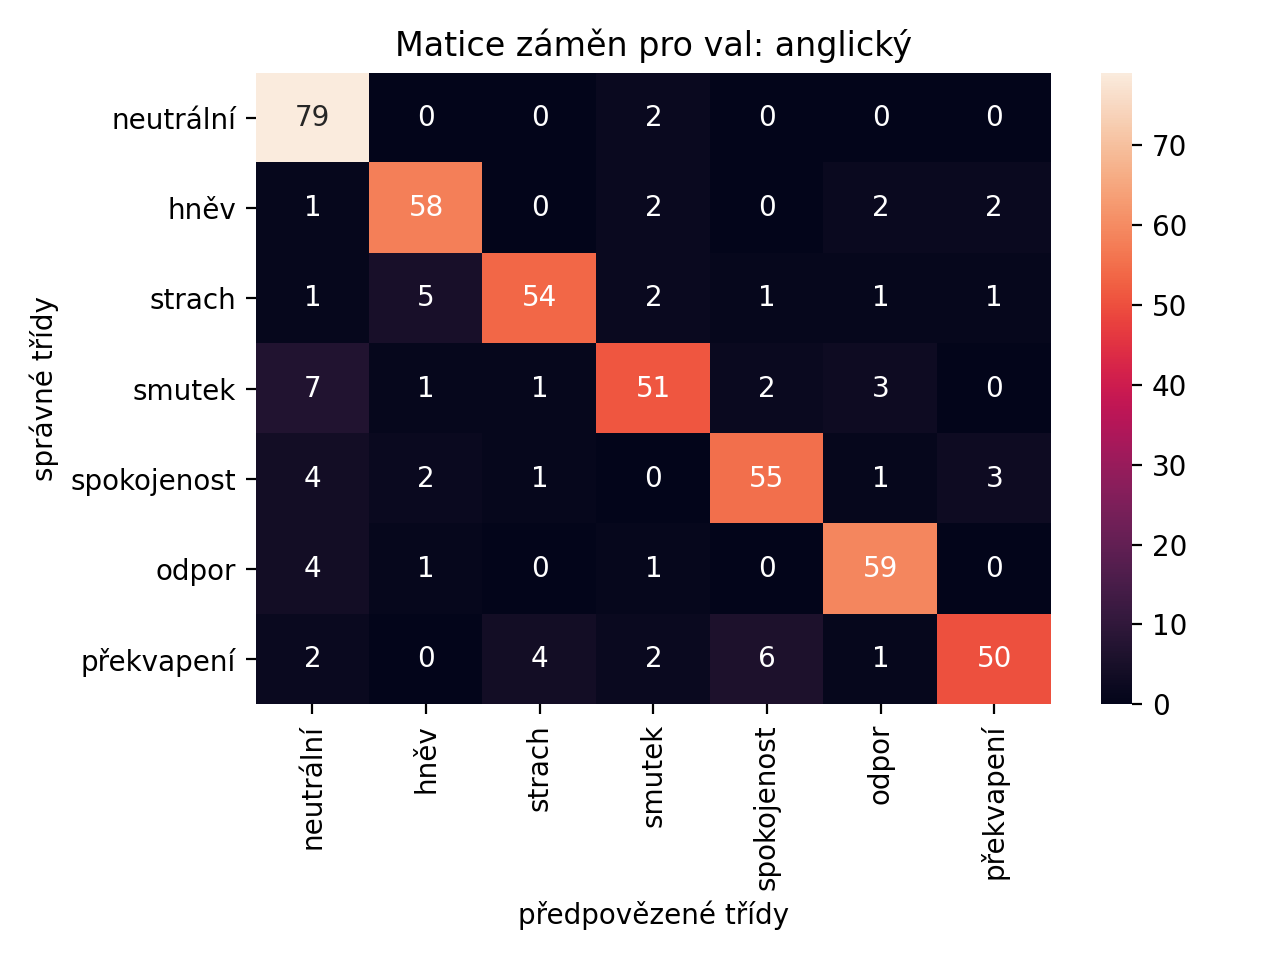
\includegraphics[scale=.5]{baseline-conf_matrix-val.png}}
\caption{Matice záměn pro validační sadu výchozího modelu}
\label{fig:conf_matrix-val-baseline}
\end{figure}
\FloatBarrier

Následně bylo provedeno několik pokusů se snahou vyladit hyperparametry modelu. Byla měněna především architektura sítě, počet a šířka vrstev. Upravovány byly také velikosti okolí vzorku. Trénování probíhalo během deseti epoch, jelikož bylo zjištěno u výchozího pokusu, že tento počet postačí pro získání představy o výkonu modelu. Kriteriální a optimalizační funkce zůstaly stejné.

\section{Změny počtu skrytých vrstev} % Grammer checked
Byly provedeny tři experimenty, jejichž cílem bylo zjistit optimální počet skrytých vrstev modelu. Byly vyzkoušeny modely se dvěma, čtyřmi a pěti vrstvami. Tři vrstvy byly vynechány, jelikož je měl výchozí model. Z grafů (viz obr. \mbox{\ref{fig:training_course-layers}} pro trénovací data lze usoudit, že s rostoucím počtem vrstev stoupá i přesnost modelu a zároveň klesá ztráta. Přesnost pro vzorky na validační a testovací sadě také roste s počtem skrytých vrstev. Nicméně s ní vzrůstá i ztráta, která by měla naopak klesat. Průběh ztráty u modelů se třemi a více vrstvami se příliš nemění. Při počtu dvou vrstev se model učí pomaleji, ale zároveň neroste v takové míře ztráta. Nejlepších výsledků dosáhl model s pěti vrstvami.
\extend{jaká byla dosažena nejlepší acc na test/valid datech a pro jakou síť? jaké je srovnání s baseline?}

\begin{table}[htb]
\centering
\caption{Přehled nejlepších výsledků pro různé počty skrytých vrstev}
\resizebox{\textwidth}{!}{\begin{tabular}{| c | c | c | c | c | c |} 
\hline
\multicolumn{1}{|c|}{\multirow{2}{*}{\thead{počet skrytých vrstev}}} & \multicolumn{1}{c|}{\thead{Trénovací sada}} & \multicolumn{2}{c|}{\thead{Validační sada}} & \multicolumn{2}{c|}{\thead{Testovací sada}} \\ 
\cline{2-6}
\multicolumn{1}{|c|}{} & \multicolumn{1}{c|}{\thead{Přesnost \\ pro vzorek}} & \multicolumn{1}{c|}{\thead{Přesnost \\ pro vzorek}} & \multicolumn{1}{c|}{\thead{Přesnost \\ pro nahrávku}} & \multicolumn{1}{c|}{\thead{Přesnost \\ pro vzorek}} & \multicolumn{1}{c|}{\thead{Přesnost \\ pro nahrávku}} \\ 
\hline
2 & 79,3 \% & 58,7 \% & 87,2 \% & 57,8 \% & 86,6 \% \\
3 (výchozí model) & 83,1 \% & 58,1 \% & 87 \% & 58 \% & 86,6 \% \\
4 & 84,4 \% & 59,5 \% & 88,7 \% & 58,3 \% & 86,6 \% \\
5 & 85 \% & 59,3 \% & 88,3 \% & 58,4 \% & 87,8 \% \\
\hline
\end{tabular}}
\label{tab:best_results}
\end{table}
\FloatBarrier

\begin{figure}[!htbp]
\centerline{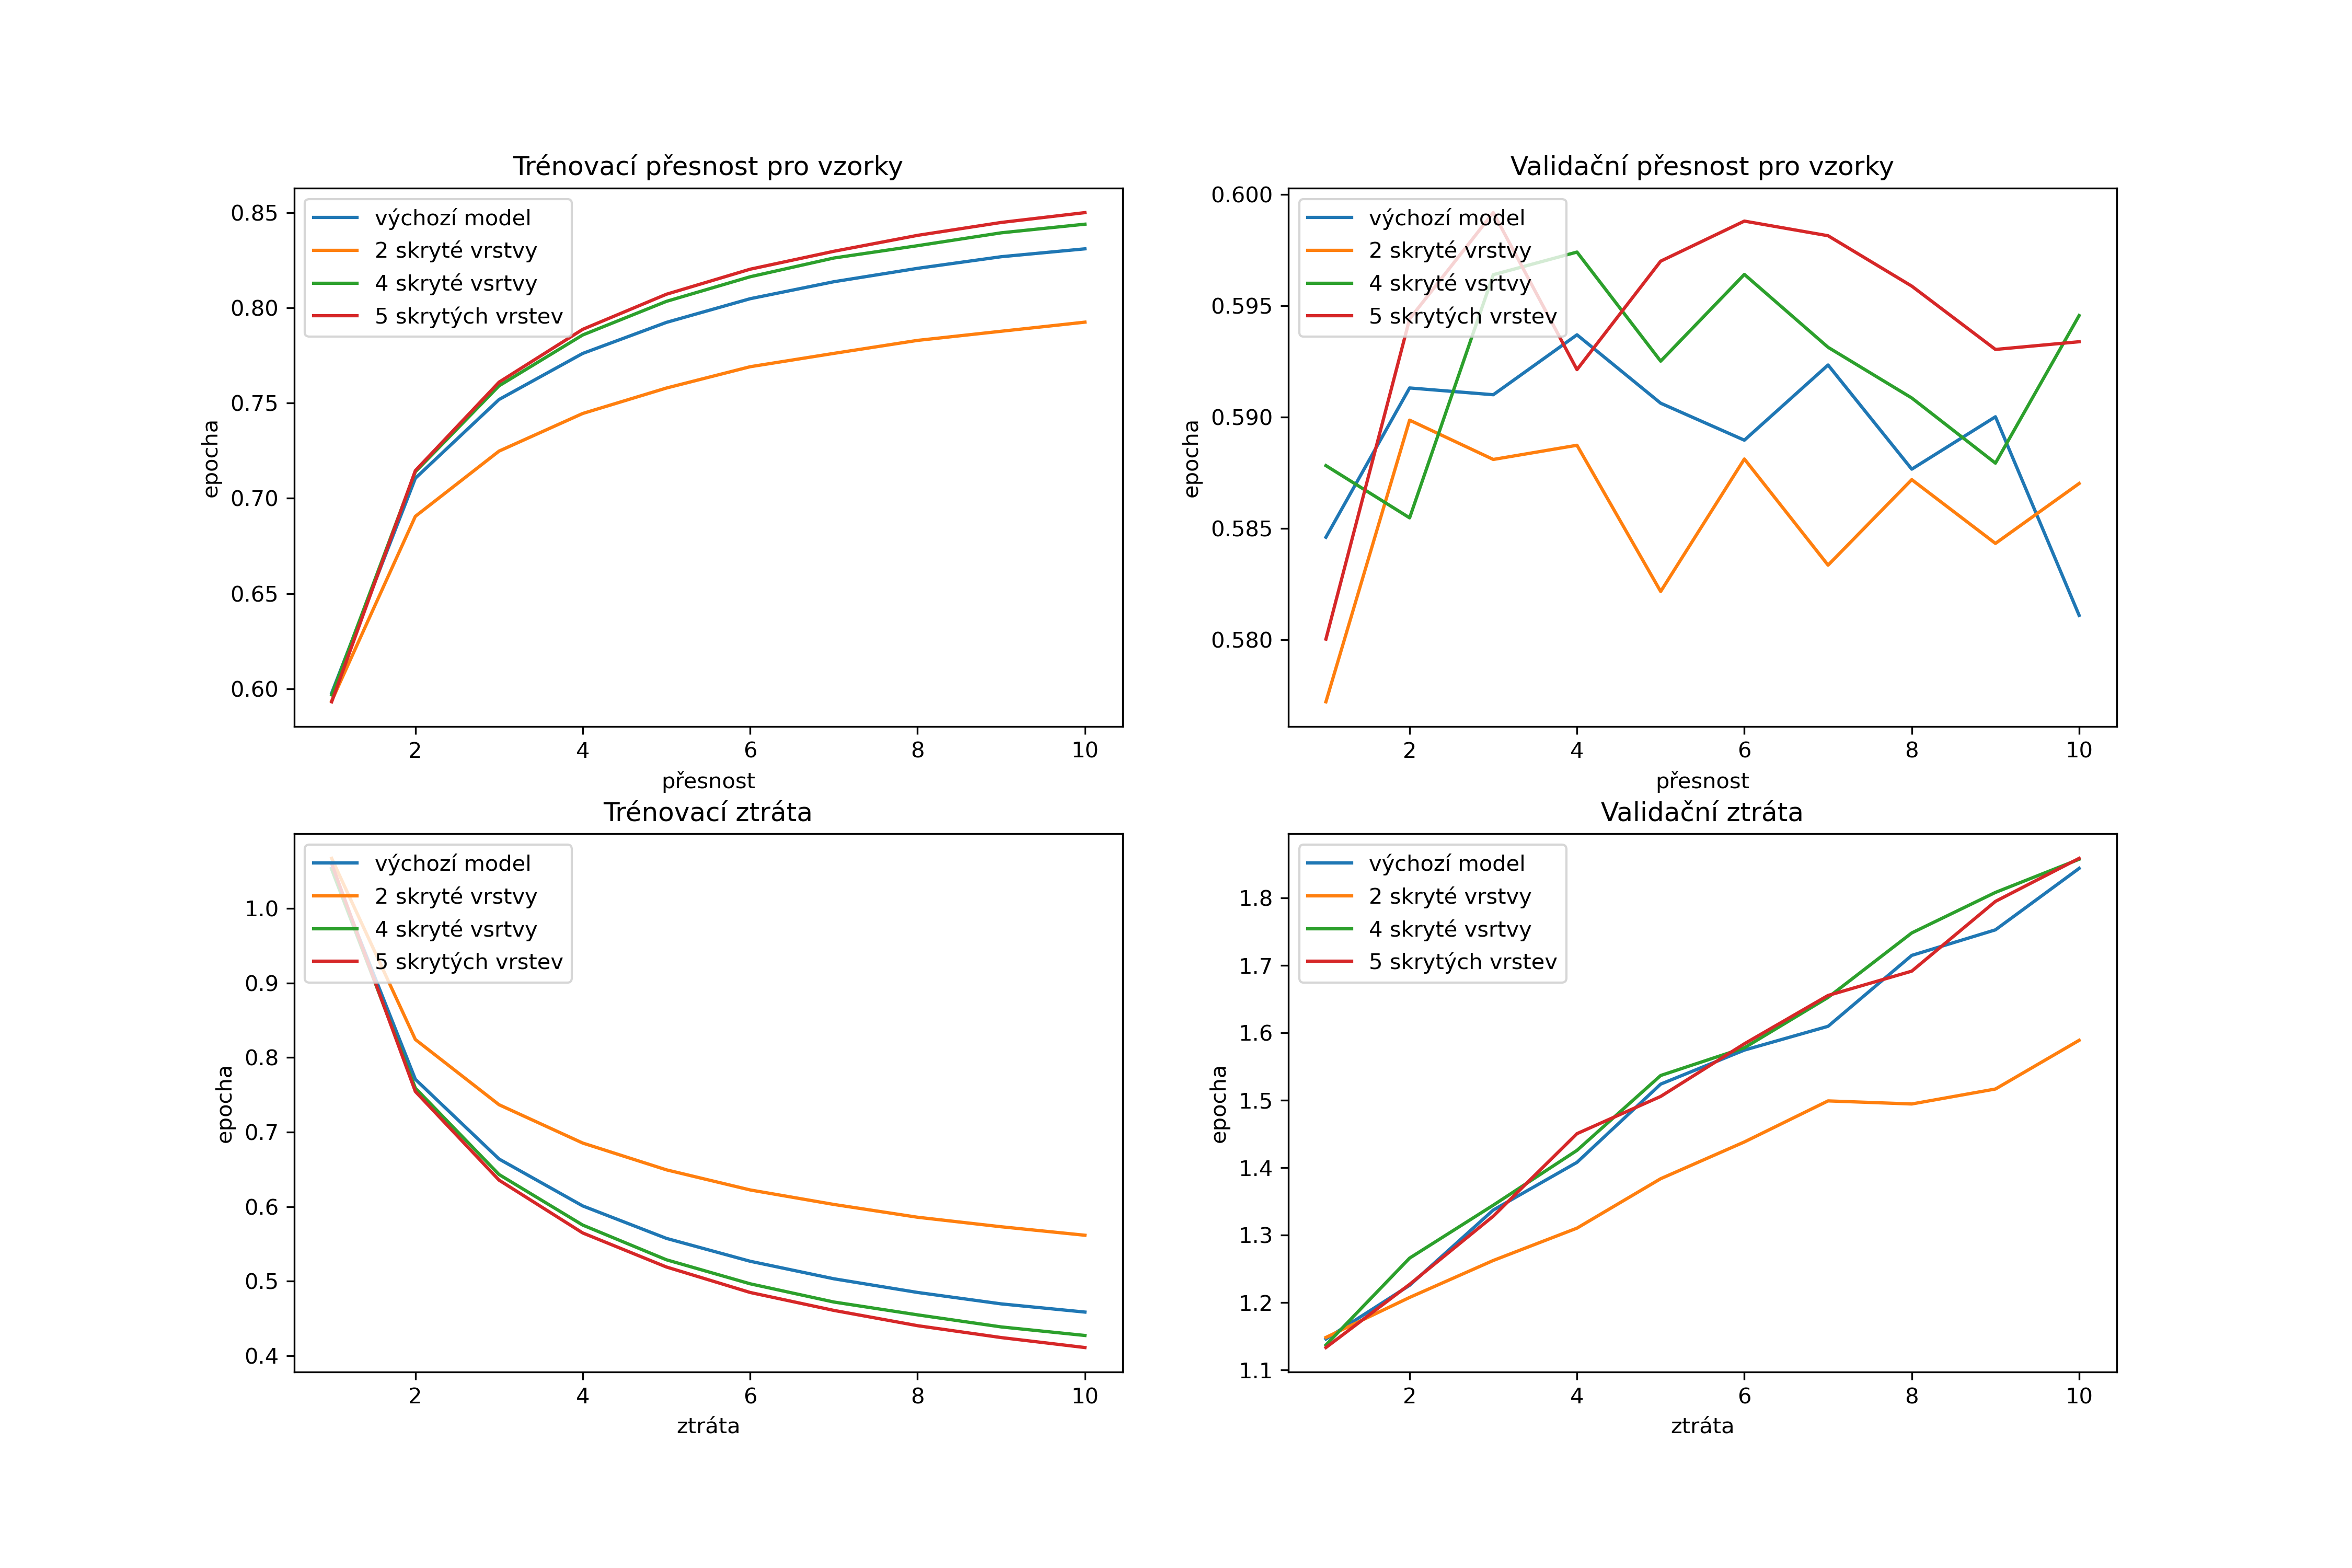
\includegraphics[scale=.5]{training_course-layers.png}}
\caption{Přehled průběhu trénování pro různé počty skrytých vrstev}
\label{fig:training_course-layers}
\end{figure}
\FloatBarrier

\section{Změny velikosti okolí vzorku} % Grammer checked
Velikost okolí vzorku bylo možné také upravovat. Celkem byly provedeny čtyři pokusy, při nichž velikost okolí pro pravou a levou stranu nabývala hodnot 5, 10, 30 a 50. Z průběhu grafů (viz obr. \mbox{\ref{fig:training_course-margin}} pro trénovací datovou sadu lze usoudit, že se zvyšujícím se okolí stoupá přesnost a klesá ztráta modelu. U validační sady přesnost pro vzorky stoupá stejným způsobem jenom pomaleji, zároveň však stoupá ztráta modelu. S ohledem na ztrátu modelu a přesnost pro vzorky jsou nejlepší modely s okolím 15 a 30.
\extend{kolik vrstev teda používáš?}
\extend{zase chybí konkrétní hodnoty a zhodnocení, co je nejlepší}
\note{přináší tu něco ty grafy z trénování, nestačily by jen validační?}

\begin{table}[htb]
\centering
\caption{Přehled nejlepších výsledků pro různé velikosti okolí}
\resizebox{\textwidth}{!}{\begin{tabular}{| c | c | c | c | c | c |} 
\hline
\multicolumn{1}{|c|}{\multirow{2}{*}{\thead{velikost okolí vzorku}}} & \multicolumn{1}{c|}{\thead{Trénovací sada}} & \multicolumn{2}{c|}{\thead{Validační sada}} & \multicolumn{2}{c|}{\thead{Testovací sada}} \\ 
\cline{2-6}
\multicolumn{1}{|c|}{} & \multicolumn{1}{c|}{\thead{Přesnost \\ pro vzorek}} & \multicolumn{1}{c|}{\thead{Přesnost \\ pro vzorek}} & \multicolumn{1}{c|}{\thead{Přesnost \\ pro nahrávku}} & \multicolumn{1}{c|}{\thead{Přesnost \\ pro vzorek}} & \multicolumn{1}{c|}{\thead{Přesnost \\ pro nahrávku}} \\ 
\hline
5 & 66,2 \% & 52,4 \% & 88,5 \% & 52,5 \% & 86,6 \% \\
15 & 76,6 \% & 57,3 \% & 88,7 \% & 56 \% & 87 \% \\
25 (výchozí model) & 83,1 \% & 58,1 \% & 87 \% & 58 \% & 86,6 \% \\
30 & 85,4 \% & 60,4 \% & 87,6 \% & 58,8 \% & 84,6 \% \\
50 & 90,7 \% & 61,9 \% & 86,8 \% & 60,7 \% & 85,5 \% \\
\hline
\end{tabular}}
\label{tab:best_results}
\end{table}
\FloatBarrier

\begin{figure}[!htbp]
\centerline{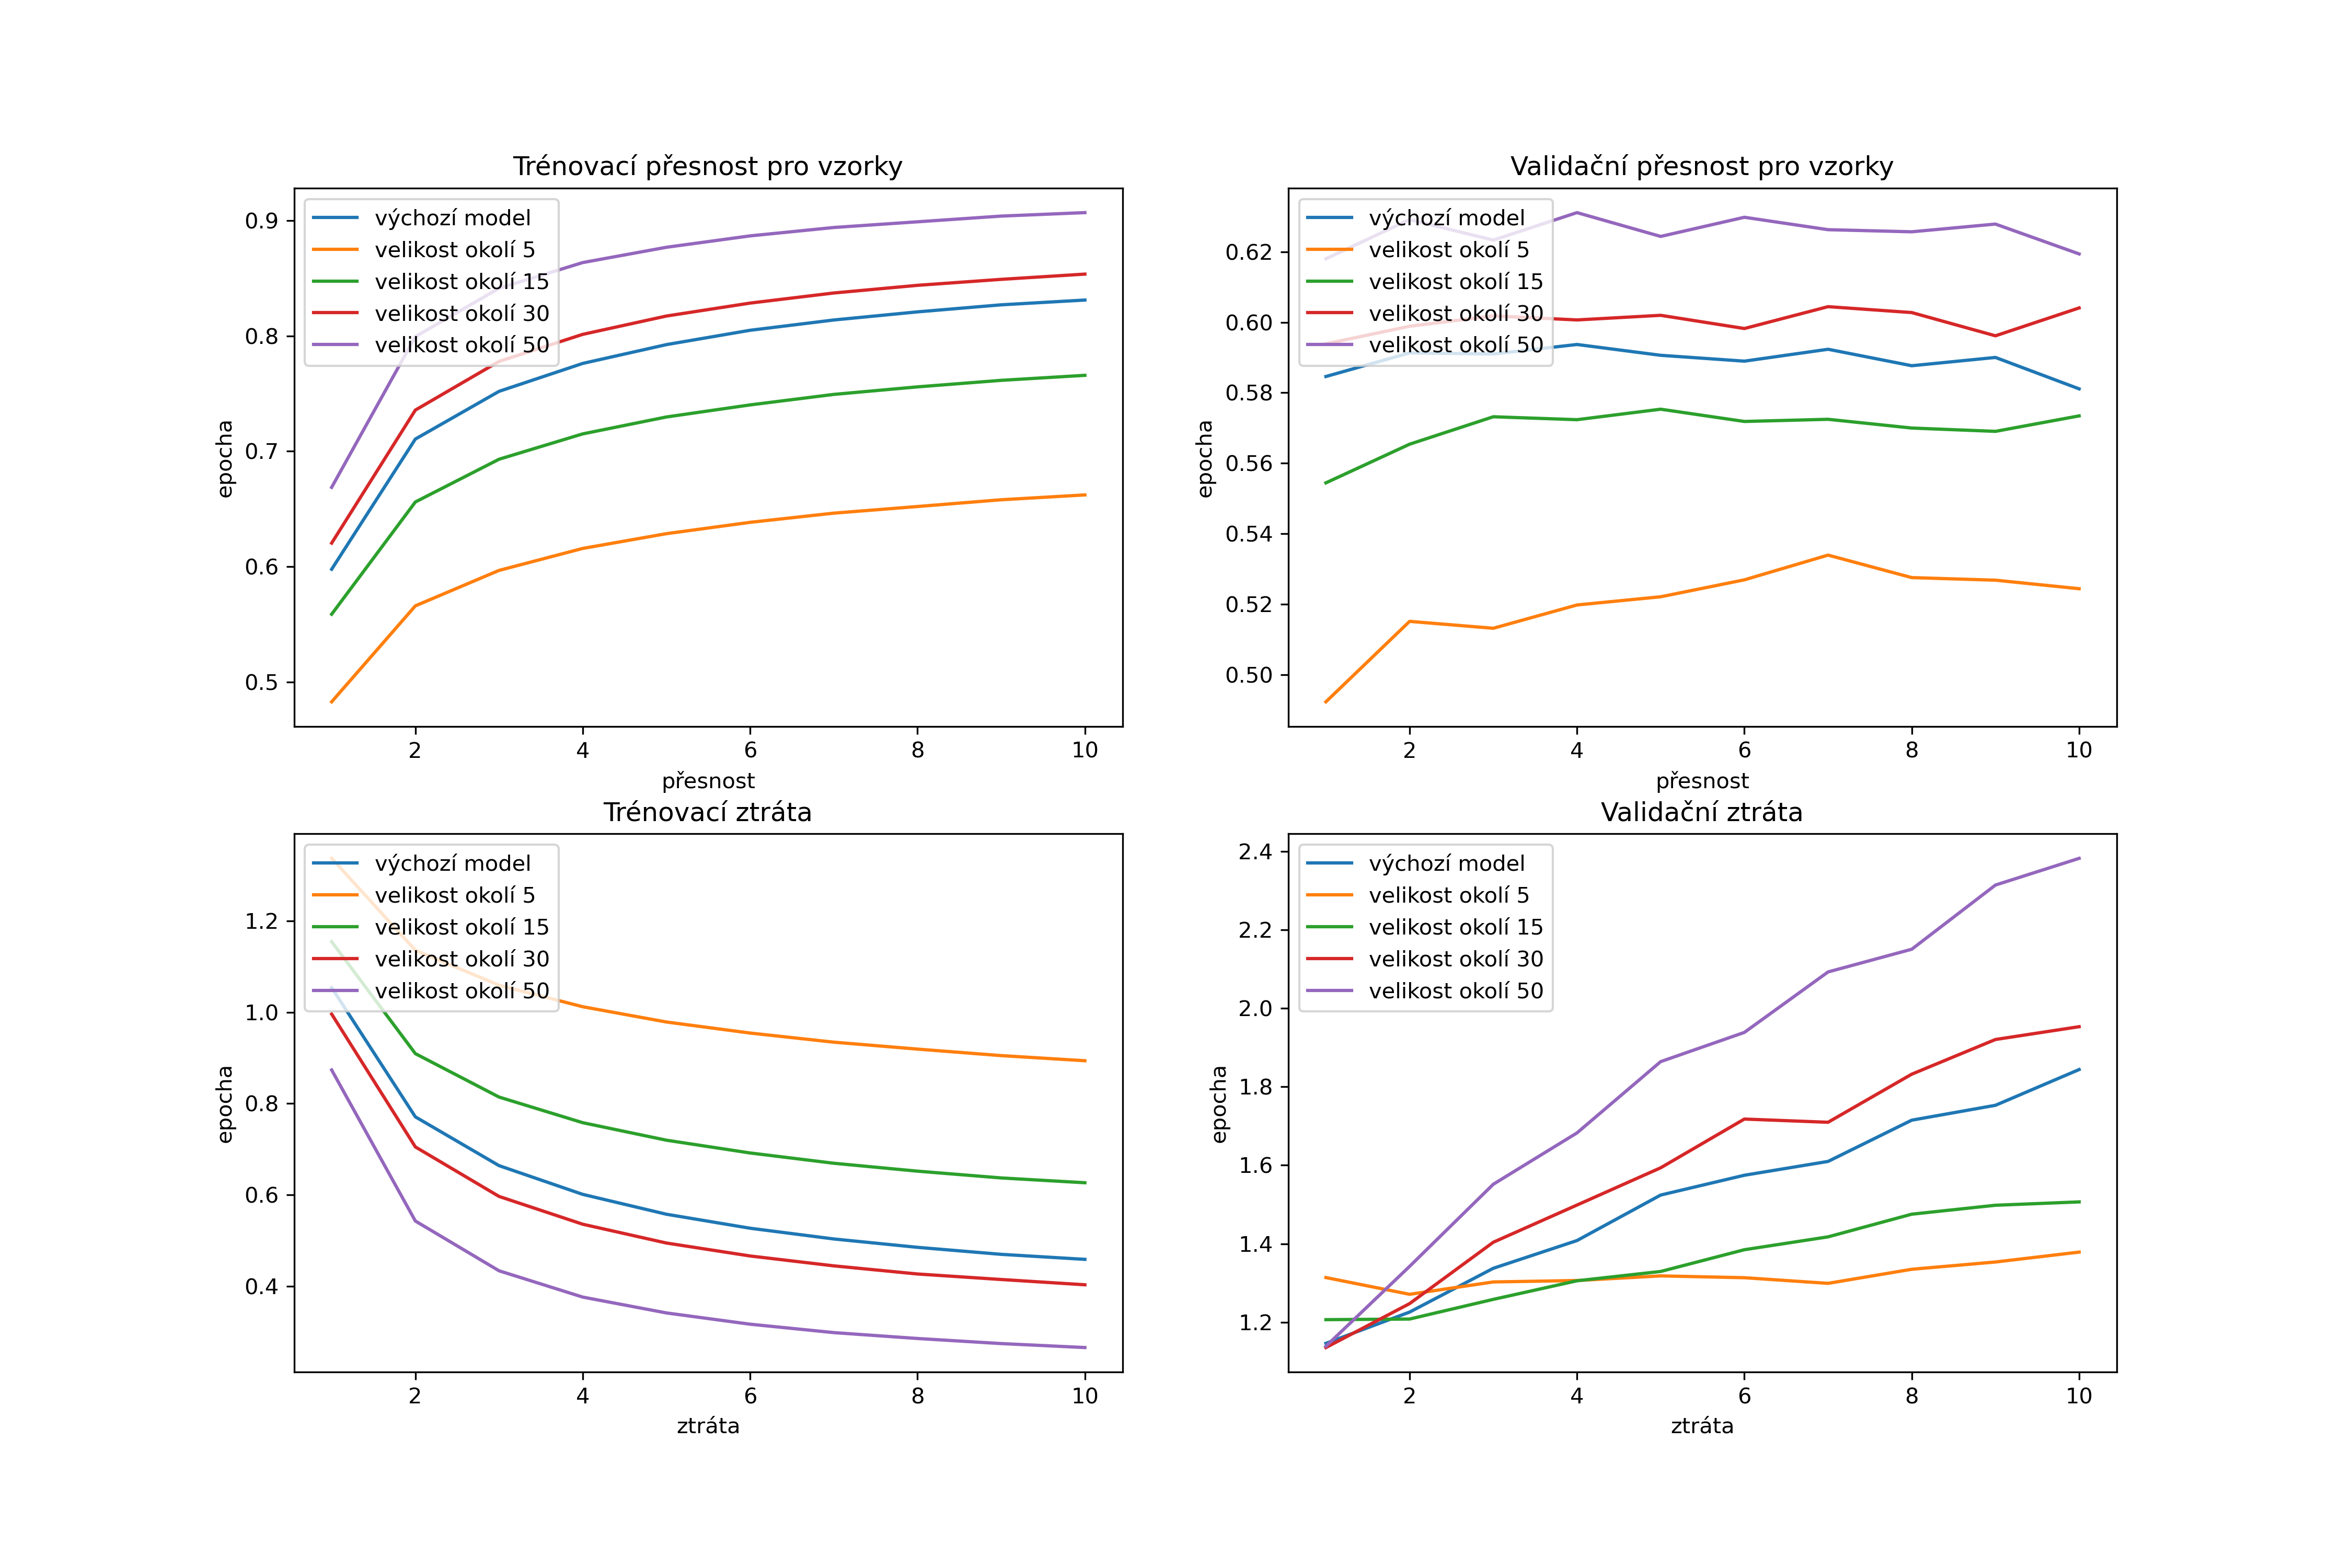
\includegraphics[scale=.5]{training_course-margin.png}}
\caption{Přehled průběhu trénování pro různé velikosti okolí}
\label{fig:training_course-margin}
\end{figure}
\FloatBarrier

\section{Změny šířky skrytých vrstev} % Grammer checked
Další parametr, který lze upravovat, je šířka skrytých vrstev modelu. Uskutečnily se čtyři experimenty, během kterých se měnila šířka skrytých vrstev. Modely měly šířku vrstev 16, 64, 256 a 512 neuronů. Při srovnání přesností pro trénovací datovou sadu si lze všimnout, že model s 16 neurony dosahuje nejnižší přesnosti kolem \mbox{50 \%}. Dále s přibývající šířkou výsledná přesnost stoupá přibližně o \mbox{10 \%}, kromě modelu s šířkou 256 a 512, kde je rozdíl mezi přesností podstatně menší. Na grafu ztráty pro validační sadu lze vidět, že ztráta klesá pro model se šířkou 16 neuronů. Pro model se šířkou 64 neuronů je ztráta téměř konstantní a pro modely se šířkou 256 a 512 výrazně stoupá. Modely se šířkou 64 a 128 neuronů dosáhly nejlepších výsledků, jelikož modely s širšími skrytými vrstvami mají větší tendenci se přeučovat.
\note{výsledky ti ale říkají, že to funguje lépe s více neurony, co říkají testovací data?}
\note{tohle používá, kolik vrstev, jaký kontext? proč zrovna tyhle a ne nějaké, co třeba fungovaly líp?}

\begin{table}[htb]
\centering
\caption{Přehled nejlepších výsledků při použití regularizace}
\resizebox{\textwidth}{!}{\begin{tabular}{| c | c | c | c | c | c |} 
\hline
\multicolumn{1}{|c|}{\multirow{2}{*}{\thead{šířka vrstev}}} & \multicolumn{1}{c|}{\thead{Trénovací sada}} & \multicolumn{2}{c|}{\thead{Validační sada}} & \multicolumn{2}{c|}{\thead{Testovací sada}} \\ 
\cline{2-6}
\multicolumn{1}{|c|}{} & \multicolumn{1}{c|}{\thead{Přesnost \\ pro vzorek}} & \multicolumn{1}{c|}{\thead{Přesnost \\ pro vzorek}} & \multicolumn{1}{c|}{\thead{Přesnost \\ pro nahrávku}} & \multicolumn{1}{c|}{\thead{Přesnost \\ pro vzorek}} & \multicolumn{1}{c|}{\thead{Přesnost \\ pro nahrávku}} \\ 
\hline
16 & 50 \% & 48,6 \% & 73,8 \% & 48,8 \% & 73,1 \% \\
64 & 69,3 \% & 56,8 \% & 84,9 \% & 56 \% & 83,6 \% \\
128 (výchozí model) & 83,1 \% & 58,1 \% & 87 \% & 58 \% & 86,6 \% \\
256 & 92,2 \% & 61,5 \% & 89,6 \% & 59,7 \% & 86,8 \% \\
512 & 94,8 \% & 62,3 \% & 89,5 \% & 60,4 \% & 88,5 \% \\
\hline
\end{tabular}}
\label{tab:best_results}
\end{table}
\FloatBarrier

\begin{figure}[!htbp]
\centerline{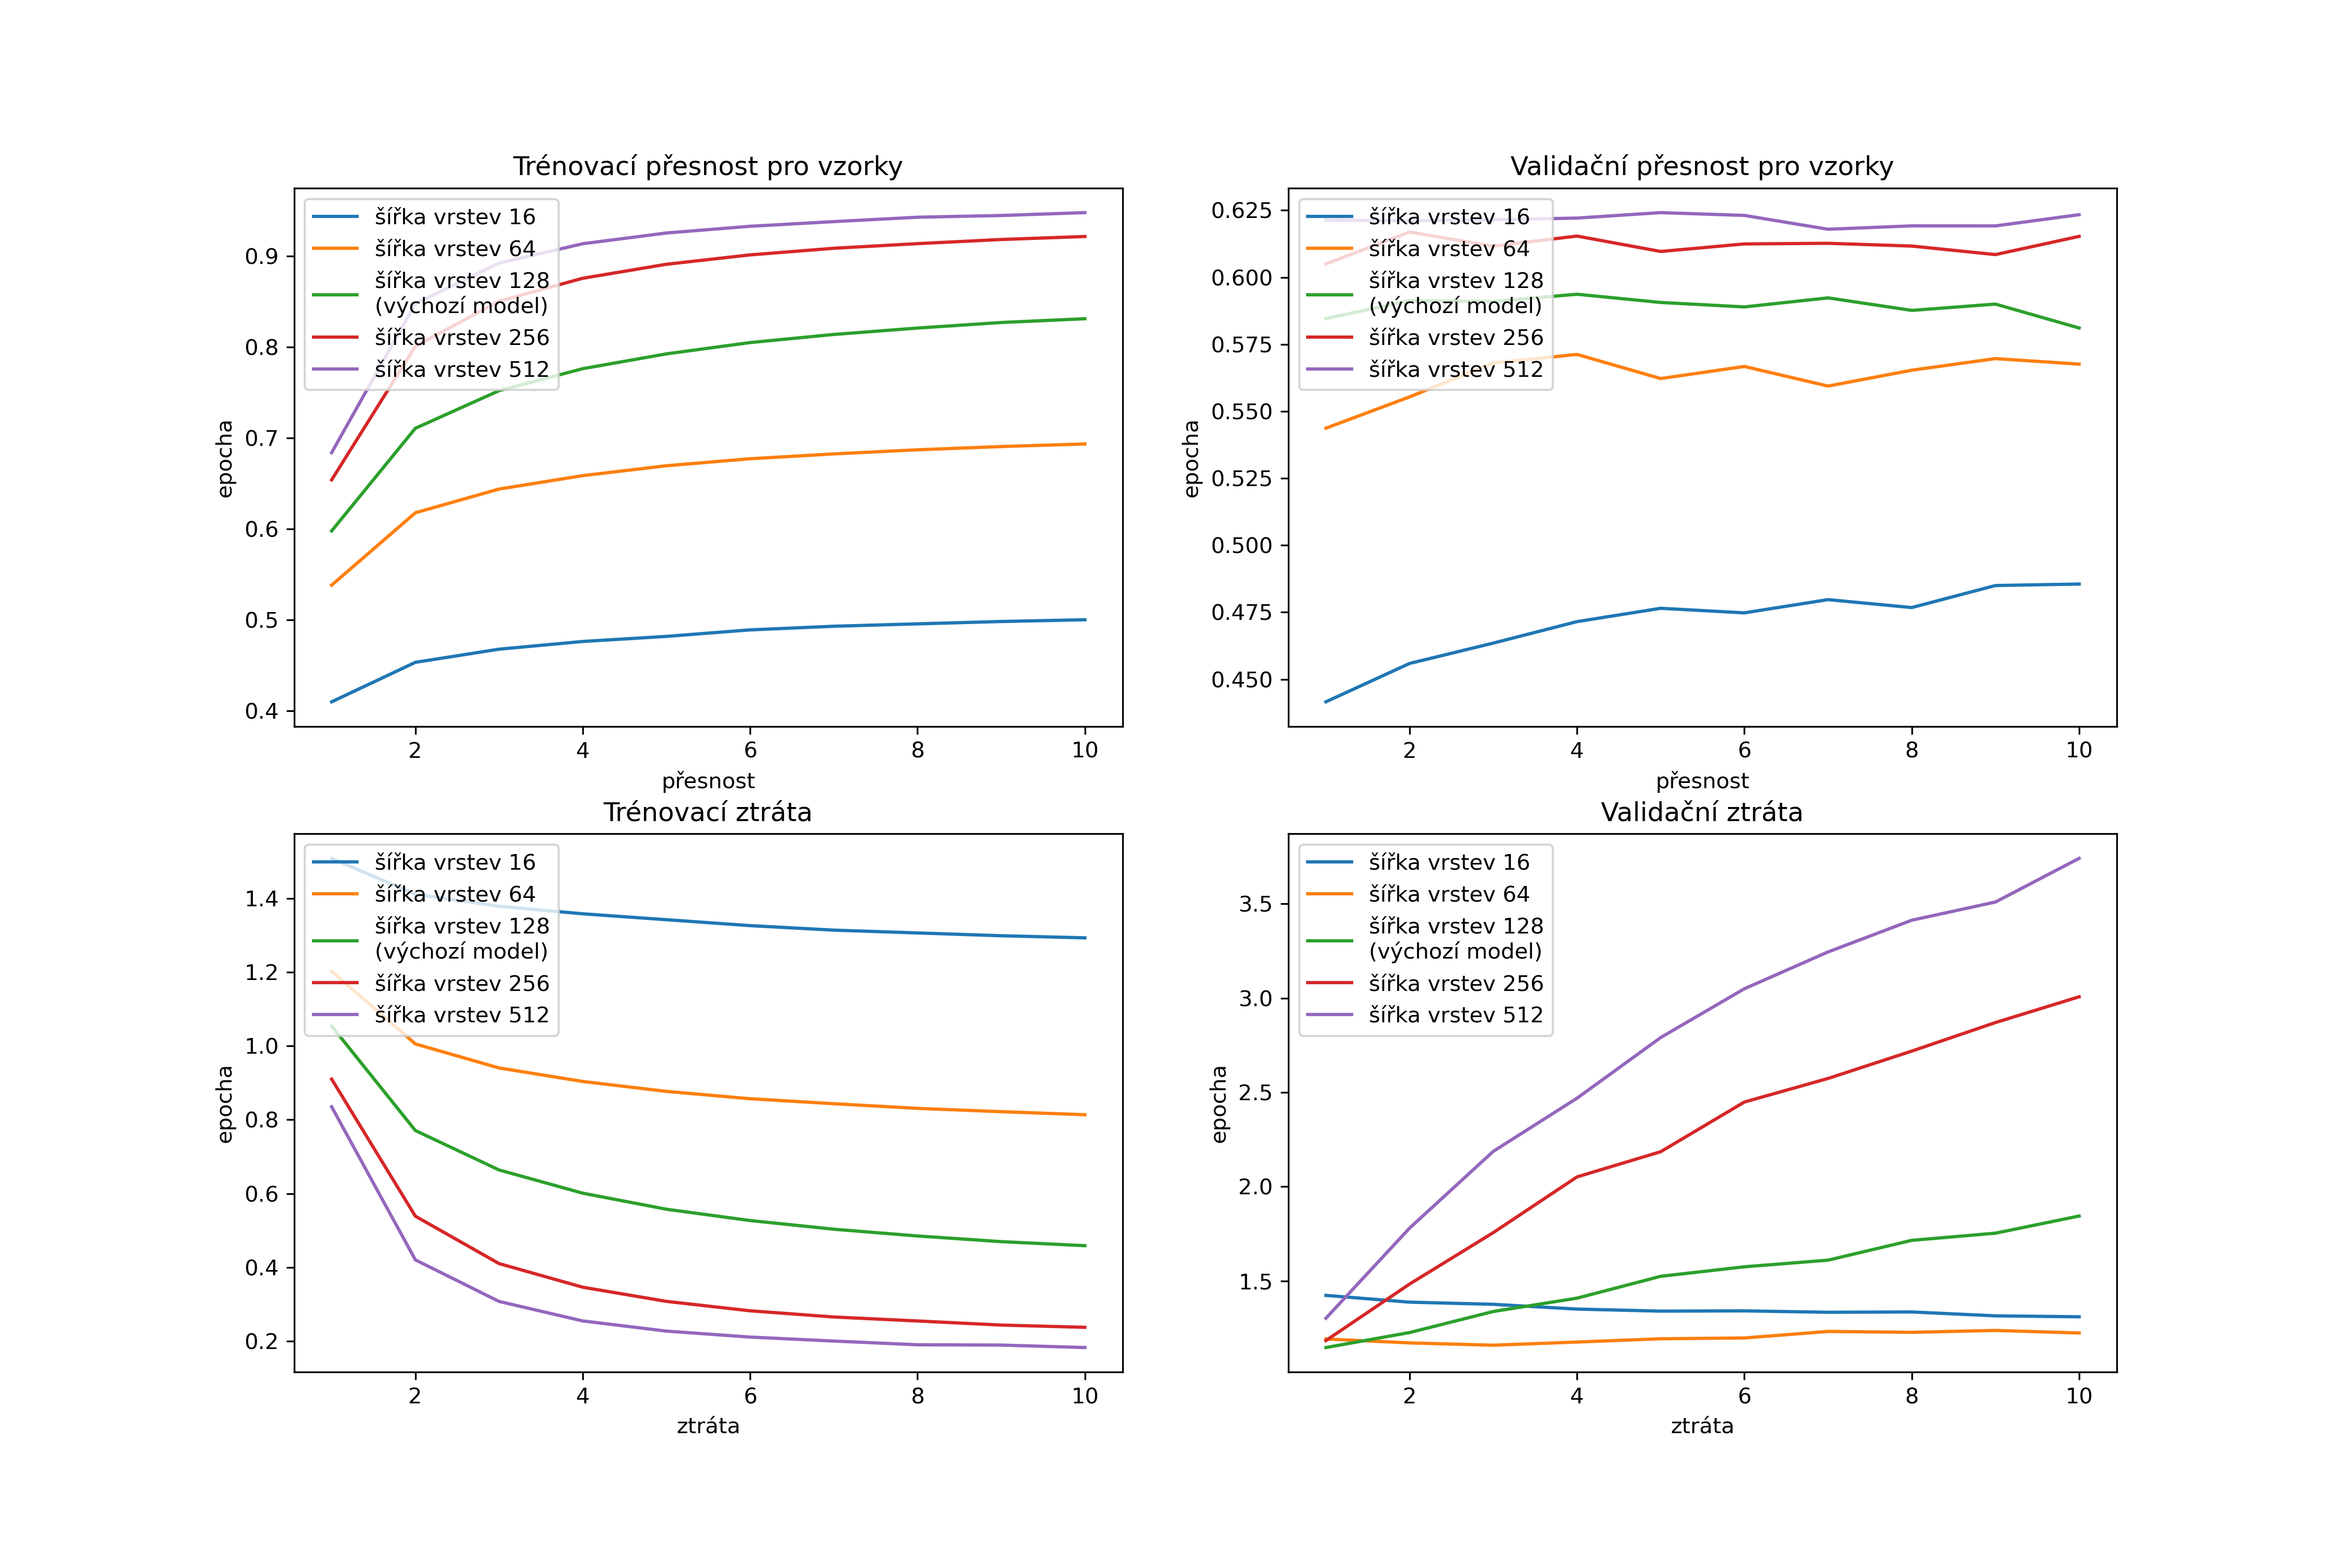
\includegraphics[scale=.5]{training_course-width.png}}
\caption{Přehled průběhu trénování při použití regularizace}
\label{fig:training_course-width}
\end{figure}
\FloatBarrier

\section{Omezení počtu emocí} % Grammer checked
V další řadě experimentů byly měněny počty emocí. \extend{uvést motivaci pro méně emocí}
Při experimentu se čtyřmi emocemi byly sjednoceny emoce hněvu a odporu na hněv, překvapení a spokojenost na spokojenost, smutek a strach na smutek. Se třemi emocemi byly rozlišovány pouze neutrální stav, negativní a pozitivní emoce. Mezi pozitivní emoce patřila spokojenost s překvapením a mezi negativní emoce hněv, odpor, smutek a strach. Z grafů (viz obr. \mbox{\ref{fig:training_course-emotion_reduction}} pro trénovací sadu lze usoudit, že s menším počtem emocí stoupá přesnost a zároveň klesá ztráta modelu. V grafech pro validační sadu lze zpozorovat, že přesnost pro vzorky s ubývajícím počtem emocí roste, ale její průběh je konstantní. Ztráta u jednotlivých modelů lineárně roste.
\note{co se tady vůbec používá za síť?}

\begin{figure}[!htbp]
\centerline{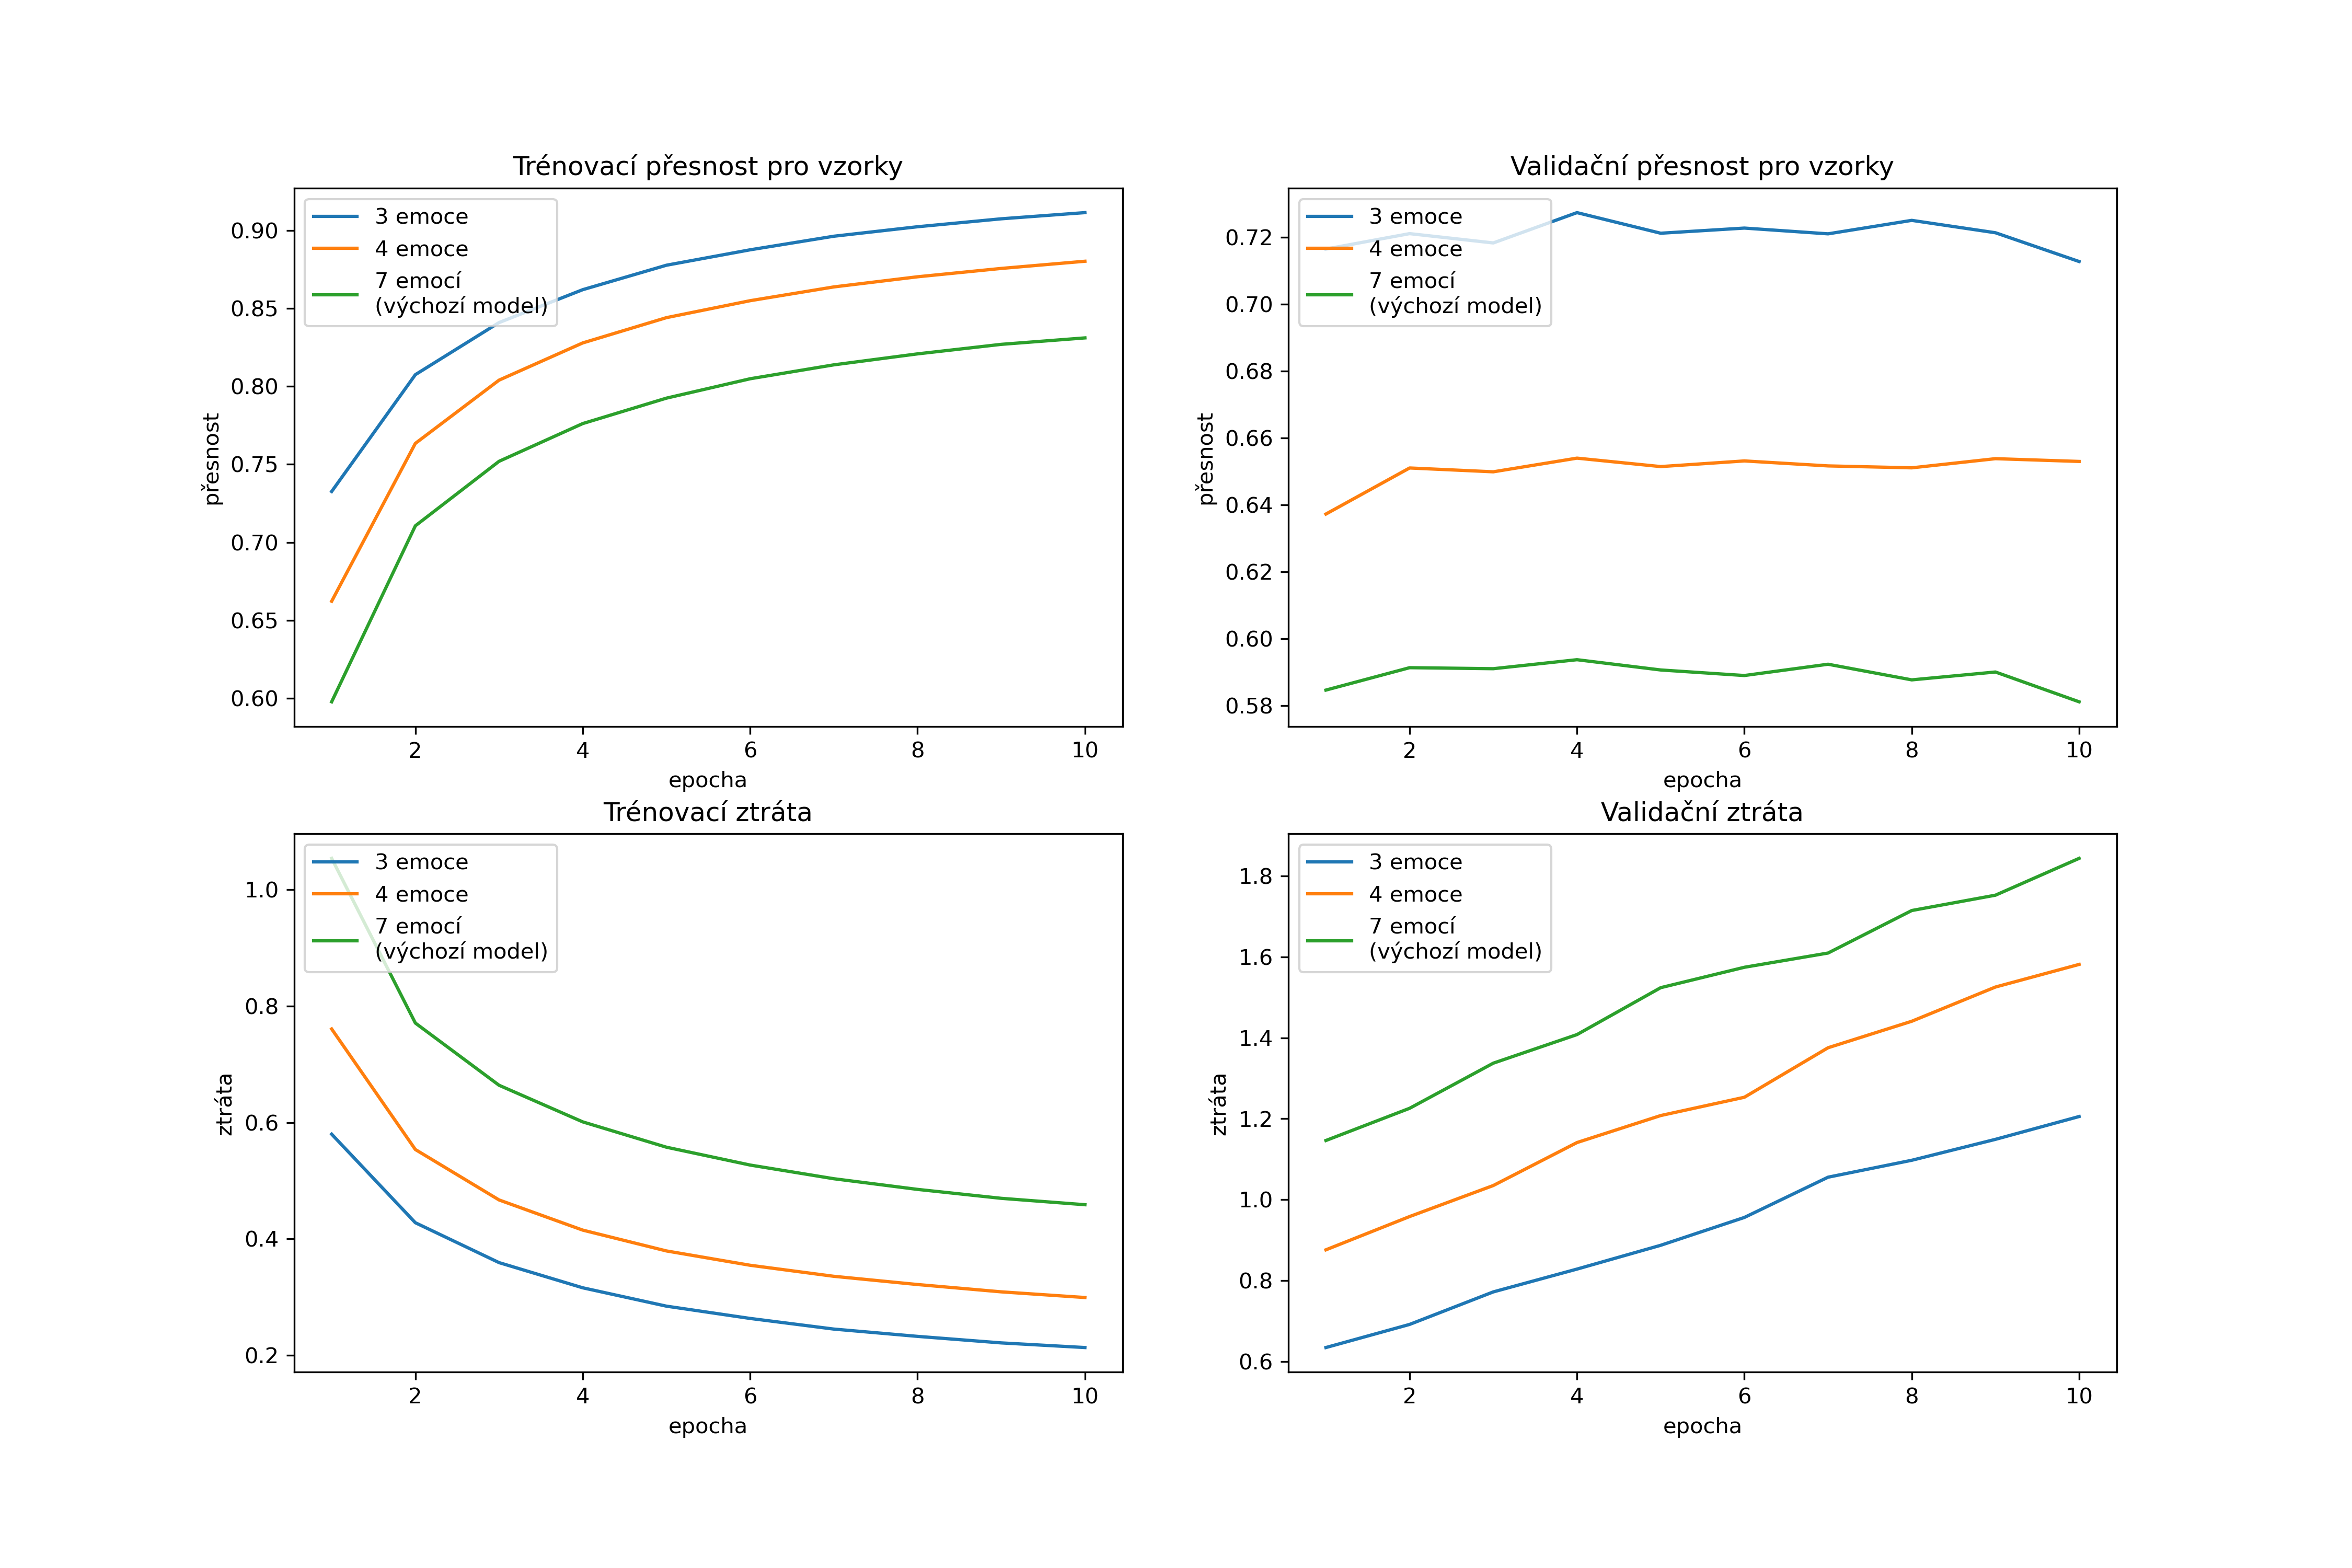
\includegraphics[scale=.5]{training_course-emotion_reduction.png}}
\caption{Přehled průběhu trénování pro různý počet emocí}
\label{fig:training_course-emotion_reduction}
\end{figure}
\FloatBarrier

Počet nahrávek pro jednotlivé třídy je mnohem vyrovnanější při klasifikaci do čtyřech tříd oproti klasifikaci do tří tříd. Při sloučení tříd pro klasifikaci do tří tříd byla největší část nahrávek umístěna do negativní třídy (viz obr. \mbox{\ref{fig:3_emotions-conf_matrix-val}}). \note{když se odkazuješ přímo na obrázek, tak je divné, že obsahuje hodnoty i mimo diagonálu}

\begin{figure}[!htbp]
\centerline{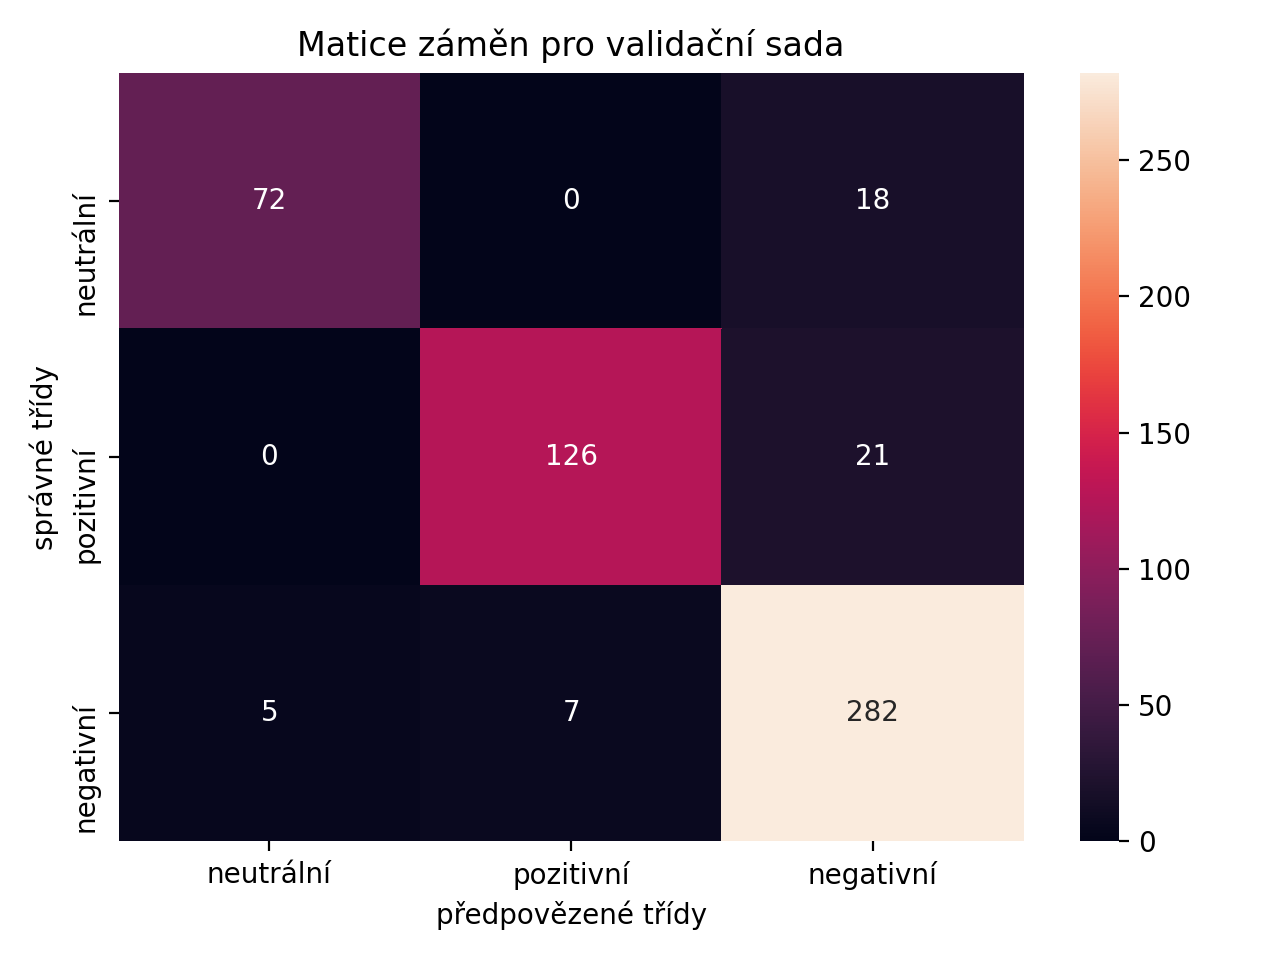
\includegraphics[scale=.5]{3_emotions-conf_matrix-val.png}}
\caption{Matice záměn pro validační data při klasifikaci tří emocí}
\label{fig:3_emotions-conf_matrix-val}
\end{figure}
\FloatBarrier

Při klasifikaci do čtyřech tříd byly nahrávky rozděleny téměř rovnoměrně do tříd hněvu, spokojenosti a smutku (viz obr. \ref{fig:4_emotions-conf_matrix-val}). O trochu méně nahrávek bylo umístěno v neutrální třídě.
\note{to stejné, asi bys měl odkázat na součet v rámci řádků nebo tak něco}

\begin{figure}[!htbp]
\centerline{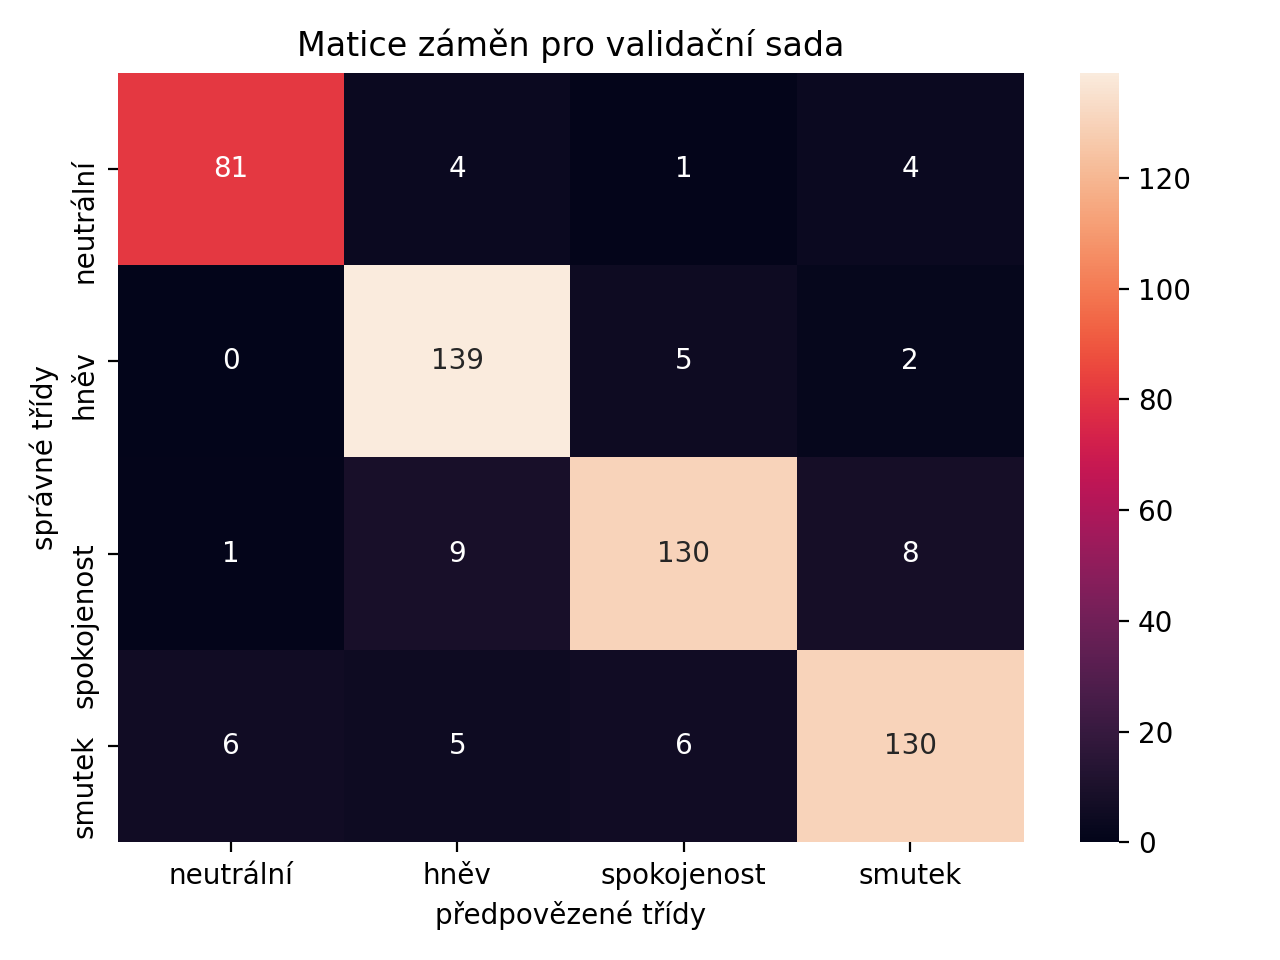
\includegraphics[scale=.5]{4_emotions-conf_matrix-val.png}}
\caption{Matice záměn pro validační data při klasifikaci čtyř emocí}
\label{fig:4_emotions-conf_matrix-val}
\end{figure}
\FloatBarrier

\begin{table}[htb]
\centering
\caption{Přehled nejlepších výsledků pro různý počet emocí}
\resizebox{\textwidth}{!}{\begin{tabular}{| c | c | c | c | c | c |} 
\hline
\multicolumn{1}{|c|}{\multirow{2}{*}{\thead{počet emocí}}} & \multicolumn{1}{c|}{\thead{Trénovací sada}} & \multicolumn{2}{c|}{\thead{Validační sada}} & \multicolumn{2}{c|}{\thead{Testovací sada}} \\ 
\cline{2-6}
\multicolumn{1}{|c|}{} & \multicolumn{1}{c|}{\thead{Přesnost \\ pro vzorek}} & \multicolumn{1}{c|}{\thead{Přesnost \\ pro vzorek}} & \multicolumn{1}{c|}{\thead{Přesnost \\ pro nahrávku}} & \multicolumn{1}{c|}{\thead{Přesnost \\ pro vzorek}} & \multicolumn{1}{c|}{\thead{Přesnost \\ pro nahrávku}} \\ 
\hline
3 & 91,1 \% & 71,3 \% & 90,4 \% & 72 \% & 91 \% \\
4 & 88 \% & 65,3 \% & 90,4 \% & 65,4 \% & 89,8 \% \\
7 (výchozí model) & 83,1 \% & 58,1 \% & 87 \% & 58 \% & 86,6 \% \\
\hline
\end{tabular}}
\label{tab:best_results}
\end{table}
\FloatBarrier

\section{Použití regularizace} % Grammer checked
Jelikož u předchozích experimentů docházelo přeučování na validační sadě, bylo vyzkoušeno několik způsobů regularizace s cílem omezení přeučování. U prvního experimentu byl přidán za aktivační funkce ve skryté vrstvě dropout s pravděpodobností \mbox{25 \%}, že se výstup vynuluje. Tento model dosahoval nižší přesnosti pro vzorek na trénovacích datech (viz obr. \mbox{\ref{fig:training_course-regularization}}) než výchozí model a ztráta klesala pomaleji. Nicméně na validačních datech měla přesnost pro vzorky tendenci růst a dosáhla vyšší přesnosti než výchozí model. Z grafu pro ztrátu je také vidět, že ztráta v průběhu trénování klesala.

% Grammer further ahead has not been checked
Pro další pokus byly skryté vrstvy výchozího modelu rozšířeny o vrstvy s normalizací dávek. Normalizace byly opět umístěny za aktivační funkce. Model dosahoval velice podobných výsledků ztráty a přesnosti na trénovacích datech. Nicméně průběhy trénovaní na validační sadě byly různé. Přesnost modelu dosáhla o \mbox{5 \%} více než na výchozím modelu a po celou dobu trénování rostla. Míra růstu ztráty byla podstatně nižší. 

U posledního experimentu byla použita kombinace předchozích technik. Za aktivační funkci byla nejdříve umístěna normalizace dávek následovaná dropout. Model dosáhl zatím nejlepších výsledků. Průběhy ztráty a přesnosti byly o trochu lepší než u modelu jenom s dropout. Avšak přesnost pro vzorky na validanční sadě stoupala rychleji a dosáhla stejných konečných výsledků jako model jenom s normalizacemi. Ztráta klesala více než u modelu s dropout. Na základě těchto výsledků byly pro další pokusy použity modely s normalizací dávek a dropout.
\note{a na jakém nastavení sítě to vlastně běží?}
\note{zase mi tu chybí ideálně nějaká shrnující tabulka}

\begin{table}[htb]
\centering
\caption{Přehled nejlepších výsledků při použití regularizace}
\resizebox{\textwidth}{!}{\begin{tabular}{| c | c | c | c | c | c |} 
\hline
\multicolumn{1}{|c|}{\multirow{2}{*}{\thead{regularizace}}} & \multicolumn{1}{c|}{\thead{Trénovací sada}} & \multicolumn{2}{c|}{\thead{Validační sada}} & \multicolumn{2}{c|}{\thead{Testovací sada}} \\ 
\cline{2-6}
\multicolumn{1}{|c|}{} & \multicolumn{1}{c|}{\thead{Přesnost \\ pro vzorek}} & \multicolumn{1}{c|}{\thead{Přesnost \\ pro vzorek}} & \multicolumn{1}{c|}{\thead{Přesnost \\ pro nahrávku}} & \multicolumn{1}{c|}{\thead{Přesnost \\ pro vzorek}} & \multicolumn{1}{c|}{\thead{Přesnost \\ pro nahrávku}} \\ 
\hline
není (výchozí) & 83,1 \% & 58,1 \% & 87 \% & 58 \% & 86,6 \% \\
dropout & 62,9 \% & 59 \% & 83,6 \% & 58,8 \% & 81,9 \% \\
normalizace dávek & 84 \% & 63,8 \% & 90,8 \% & 62,7 \% & 90,6 \% \\
dropout s normalizací dávek & 65,8 \% & 63,7 \% & 86,1 \% & 63,6 \% & 85,3 \% \\
\hline
\end{tabular}}
\label{tab:best_results}
\end{table}
\FloatBarrier

\begin{figure}[!htbp]
\centerline{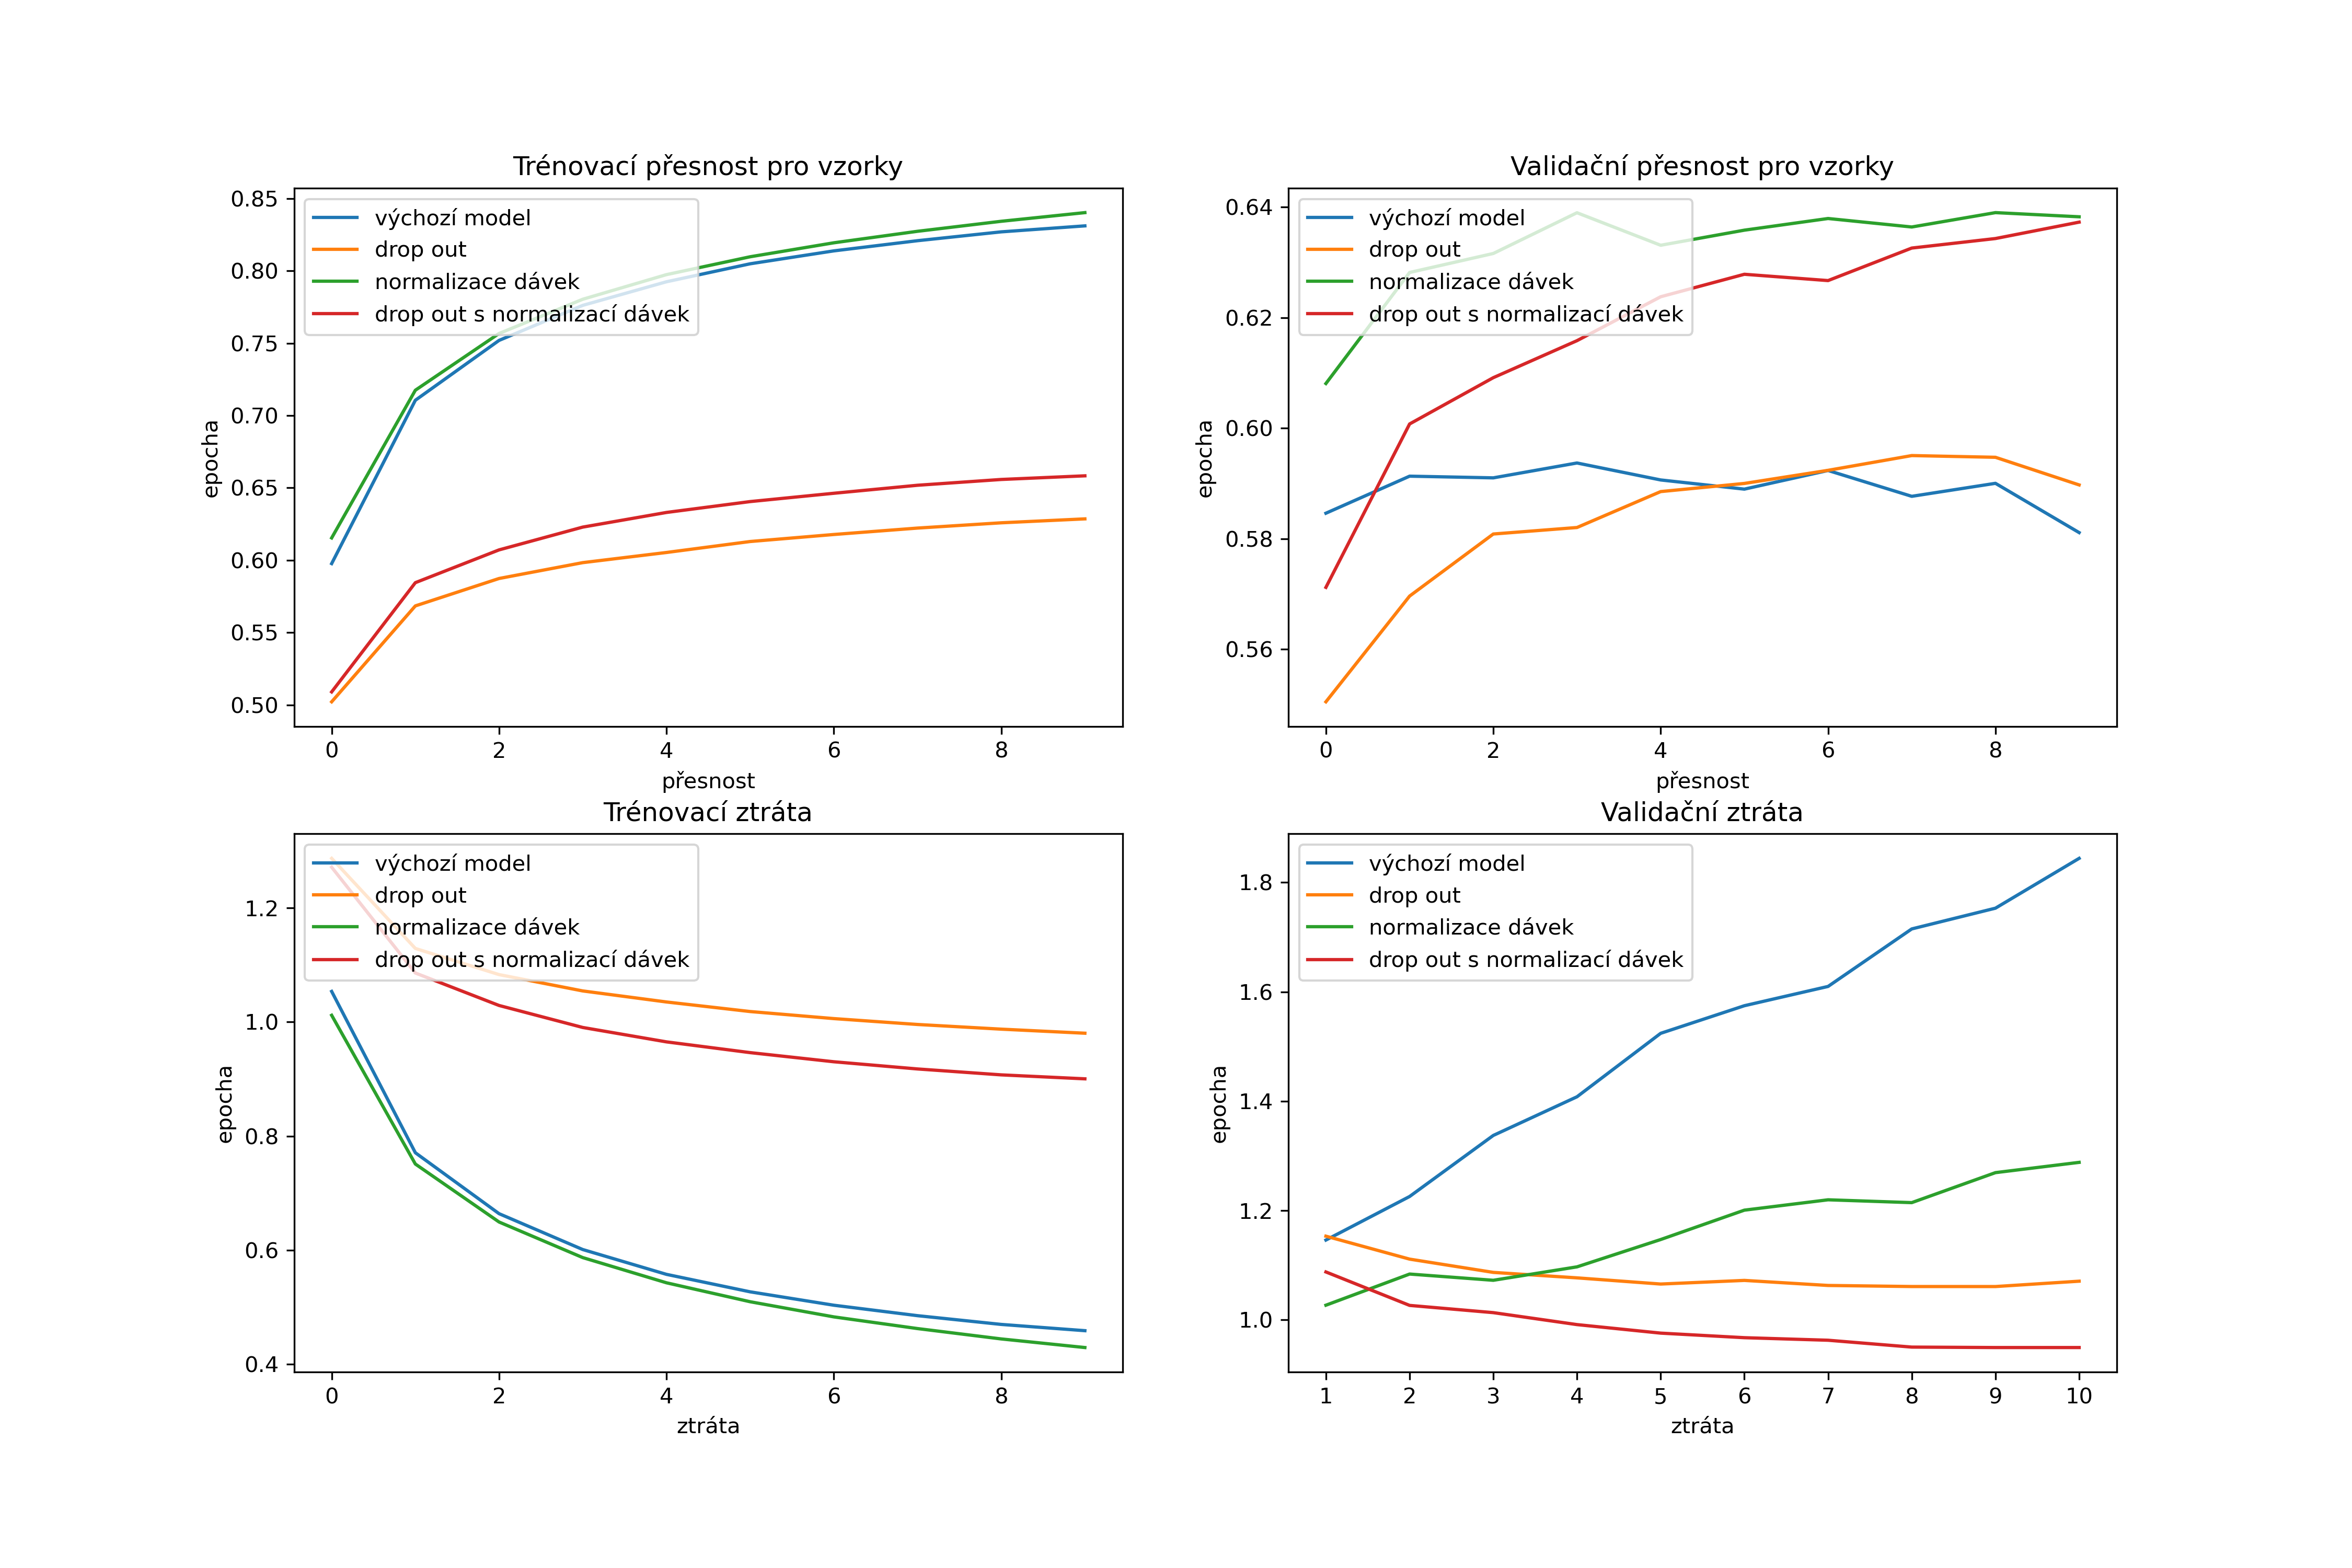
\includegraphics[scale=.5]{training_course-regularization.png}}
\caption{Přehled průběhu trénování při použití regularizace}
\label{fig:training_course-regularization}
\end{figure}
\FloatBarrier

\note{Brát poslední epochy}
\note{Natrénovat stejný finální model}
\note{Finální 10 epoch, 4 vrstvy, okolí 30, 256 neuronů, normalizace dávek}
\note{Zmínit, jak dlouho se trénoval finální}
\note{horní tabulky validační a trénovací}
\note{testovací u posledních}
\note{Změnit vzorky za nahrávky v grafech}
\note{}
\section{Finální modely}
Jako poslední byly vytvořeny finální modely pro klasifikaci do tří, čtyř a sedmi tříd. Byly použity různé modifikace modelu s normalizací dávek a dropout ve skryté vrstvě. Pro všechny počty emocí byly vyzkoušeny tři modely. Průběhy trénování jsou vykresleny v přehledu \mbox{\ref{fig:training_course-final_more}}.

\note{tohle je poprvé, co mluvíme o acc na nahrávky, což je to hlavní, co nás zajímá, protože děláš offline přístup...}
První model měl tři skryté vrstvy o šířce 64 neuronů a vzorek do sítě vstupoval s velikostí 30 pravého a levého okolí. Tento typ architektury se osvědčil při klasifikaci do tří tříd. Během 26. epochy došlo k získání nejlepších výsledků, kdy model dosáhl přesnosti pro vzorky \mbox{77,4 \%} na trénovací sadě, \mbox{73,4 \%} na validační sadě a \mbox{75,4 \%} na testovací sadě. Byla získána přesnost pro nahrávky \mbox{83,2 \%} na validační sadě a \mbox{84,7 \%} na sadě testovací.

Další model se skládal ze tří skrytých vrstev o šířce 128 neuronů s velikostí 30 pravého a levého okolí. Při klasifikaci do čtyř a sedmi tříd model vykazoval dobré výsledky, které byly překonány posledním modelem. \note{proč tu teda je?}

Model, který se nejvíce osvědčil při klasifikaci do čtyř a sedmi tříd, se skládal ze čtyř skrytých vrstev o šířce 128 neuronů a vzorek do sítě vstupoval s velikostí 50 pravého a levého okolí. Při klasifikaci do čtyř tříd měl průběh trénování větší růst u přesnosti pro vzorky a větší spád ztráty než u předchozího modelu. Nicméně měl větší tendenci se přeučovat a nejlepších výsledků dosáhl na 10. epoše, kdy byly přesnosti pro vzorky na trénovací sadě \mbox{79 \%}, na validační sadě \mbox{73,7 \%} a na testovací sadě \mbox{73,6 \%}. Přesnost pro nahrávky vystoupala u validační sady na \mbox{91,7 \%} a u testovací sady na \mbox{92,3 \%}. Model dosáhl lepších výsledků přesnosti pro nahrávky než při klasifikaci do tří tříd pravděpodobně kvůli rovnoměrnějšímu rozložení nahrávek do jednotlivých tříd. Při klasifikaci do sedmi tříd bylo dosaženo nejlepších výsledků v poslední epoše trénování. Přesnost pro vzorky vystoupala na trénovací sadě na \mbox{75,8 \%}, na sadě validační na \mbox{69,3 \%} a na testovací sadě na \mbox{68 \%}. Bylo dosaženo přesnosti pro nahrávky \mbox{90,4 \%} na sadě validační a \mbox{88,5 \%} na sadě testovací. V tabulce \mbox{\ref{tab:best_results}} jsou vypsány nejlepší výsledky finálních modelů. \note{i tyhle jsou lepší než pro 3}
\note{ty vybrané modely úplně nekorespondují s těmi předchozími experimenty nebo ano?}
\note{jak jsi je vlastně zvolil?}
\note{je trochu nefér porovnávat 3 emoce s mnohem menším modelem s více emocemi s většími modely...}

\begin{table}[htb]
\centering
\caption{Přehled nejlepších výsledků finálních modelů}
\resizebox{\textwidth}{!}{\begin{tabular}{| c | c | c | c | c | c |} 
\hline
\multicolumn{1}{|c|}{\multirow{2}{*}{\thead{Počet tříd}}} & \multicolumn{1}{c|}{\thead{Trénovací sada}} & \multicolumn{2}{c|}{\thead{Validační sada}} & \multicolumn{2}{c|}{\thead{Testovací sada}} \\ 
\cline{2-6}
\multicolumn{1}{|c|}{} & \multicolumn{1}{c|}{\thead{Přesnost \\ pro vzorek}} & \multicolumn{1}{c|}{\thead{Přesnost \\ pro vzorek}} & \multicolumn{1}{c|}{\thead{Přesnost \\ pro nahrávku}} & \multicolumn{1}{c|}{\thead{Přesnost \\ pro vzorek}} & \multicolumn{1}{c|}{\thead{Přesnost \\ pro nahrávku}} \\ 
\hline
3 & 77,4 \% & 73,4 \% & 83,2 \% & 75,4 \% & 84,7 \% \\
4 & 79 \% & 73,7 \% & 91,7 \% & 73,6 \% & 92,3 \% \\
7 & 75,8 \% & 69,3 \% & 90,4 \% & 68 \% & 88,5 \% \\
\hline
\end{tabular}}
\label{tab:best_results}
\end{table}
\FloatBarrier

\begin{figure}[!htbp]
\centerline{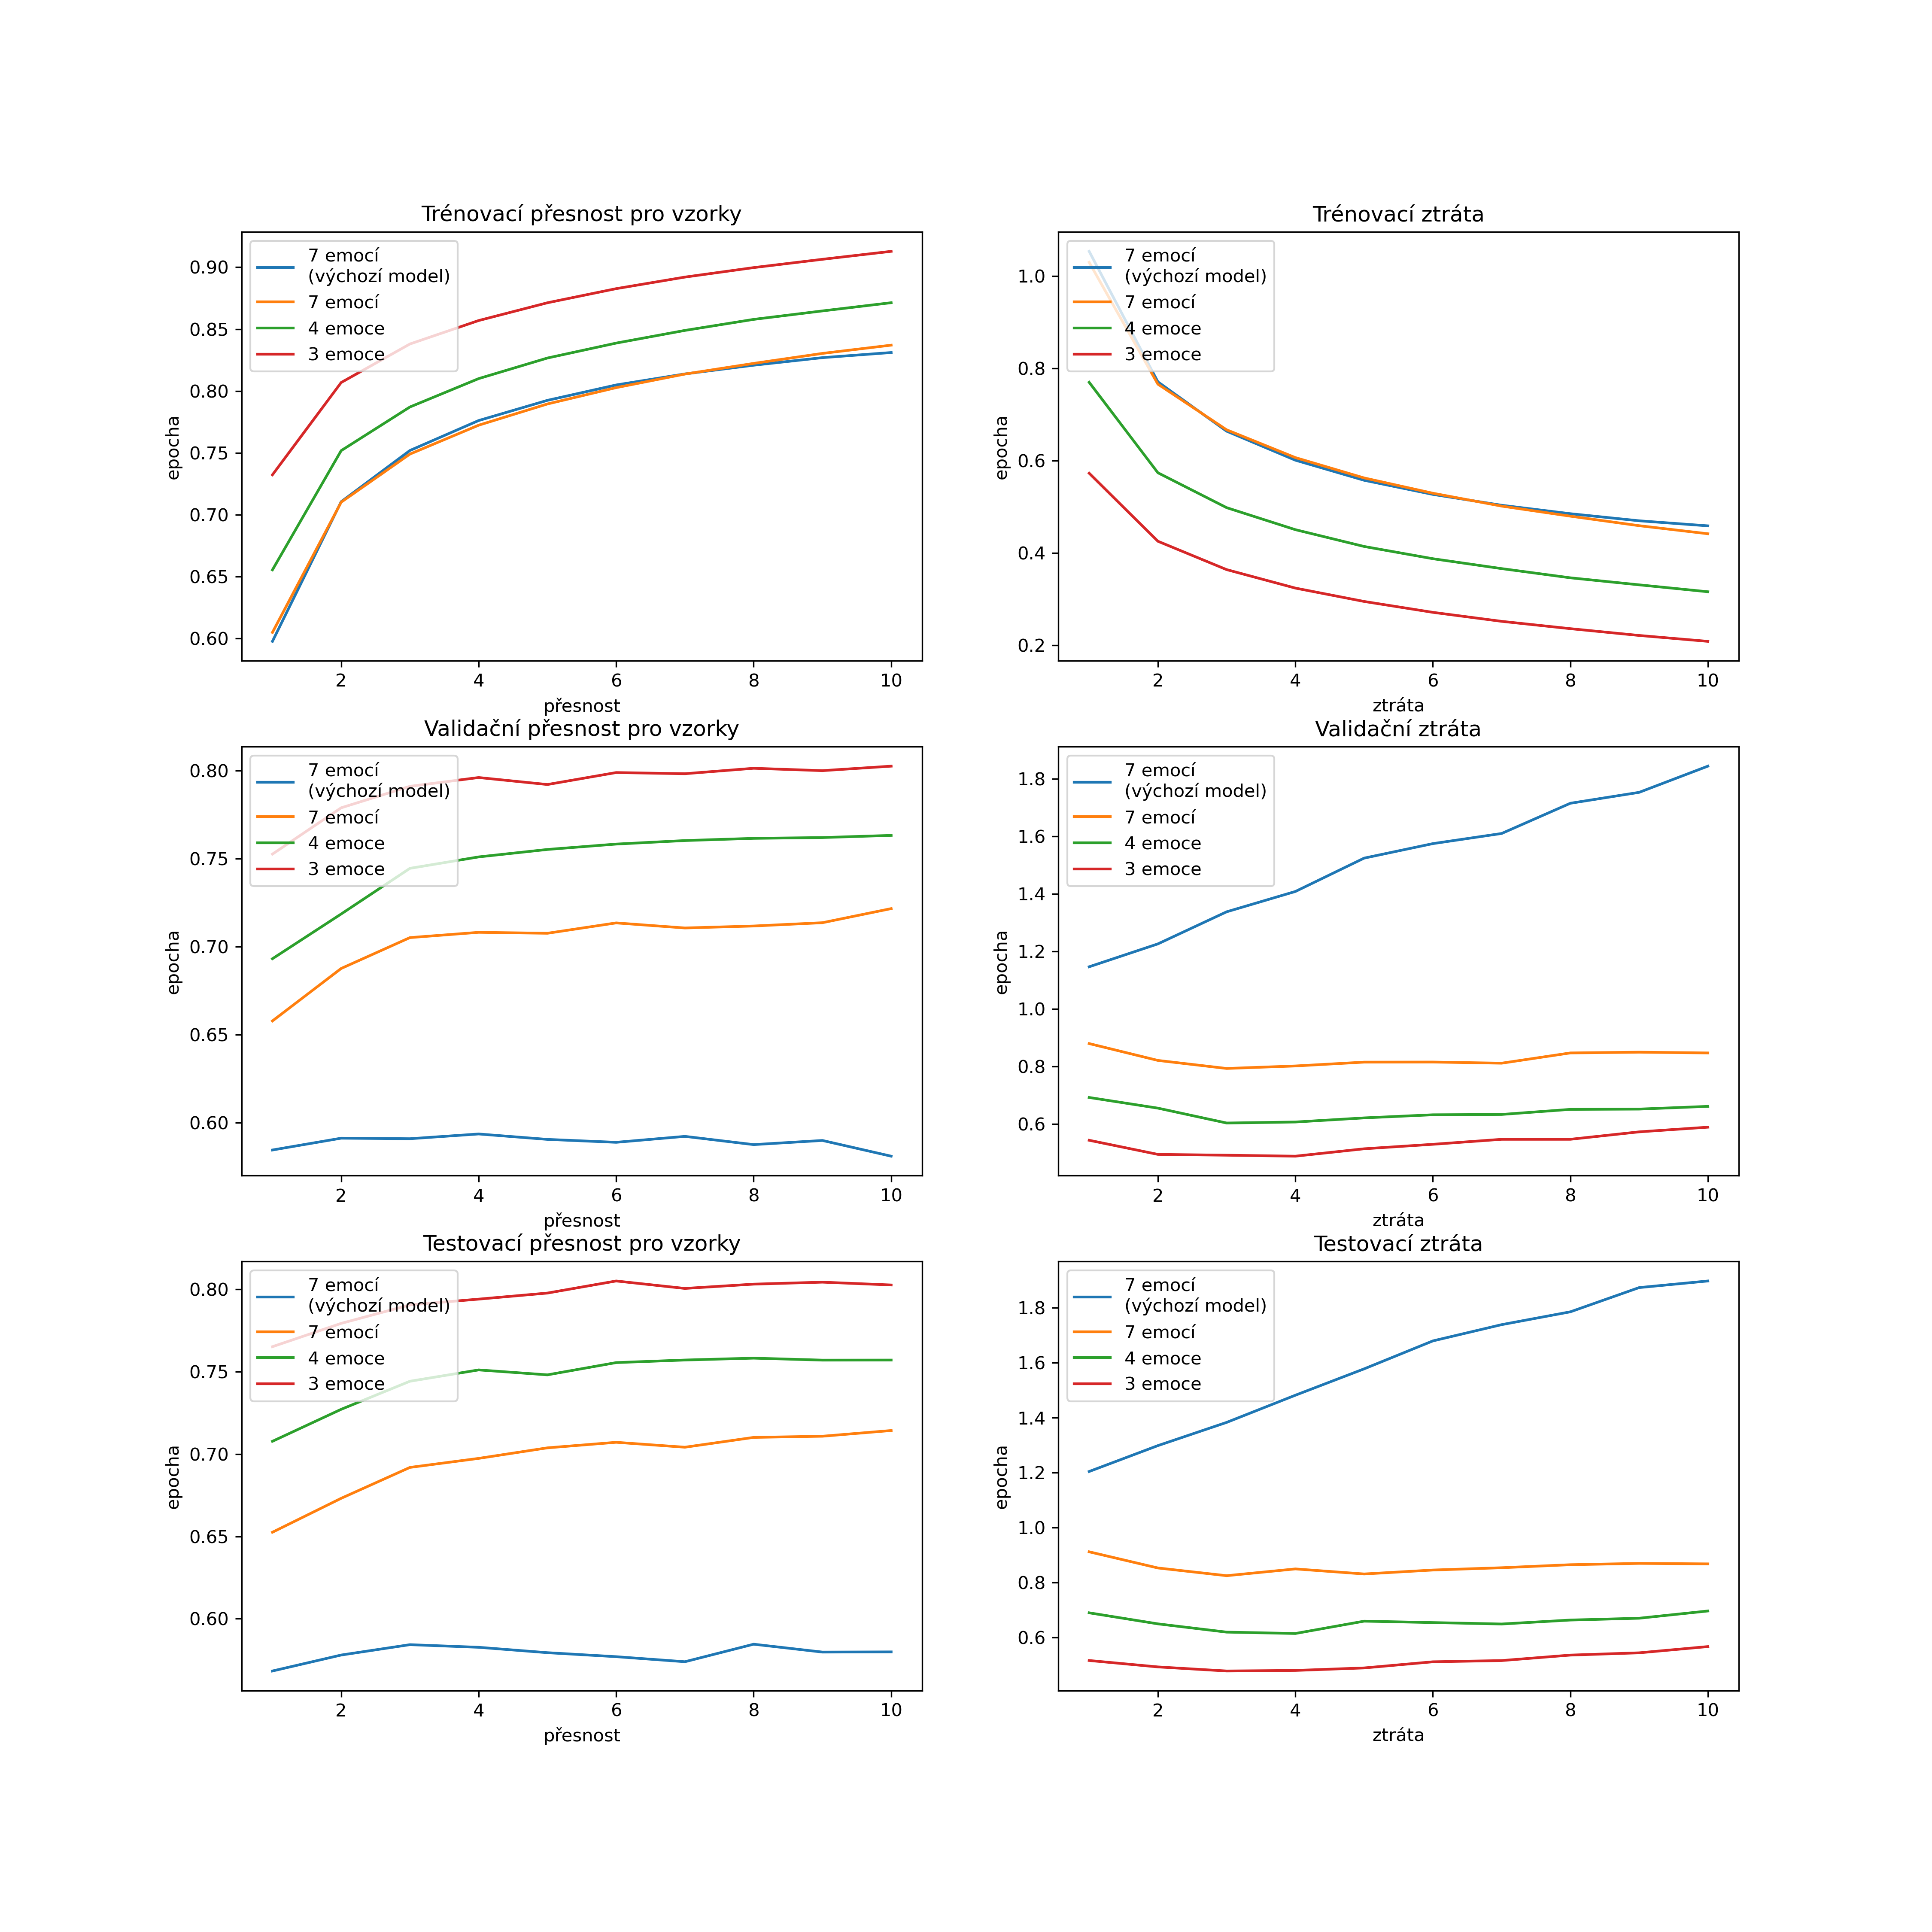
\includegraphics[scale=.5]{training_course-final_more.png}}
\caption{Přehled průběhu trénování finálních modelů}
\label{fig:training_course-final_more}
\end{figure}
\FloatBarrier

\chapter{Závěr} % Grammer checked
V teoretické části byly nejprve uvedeny emoce a hlavní dva modely pro jejich dělení. Byl popsán postup pro vytváření systému pro rozpoznávání emocí z řeči. V současném poznání byly uvedeny používané příznaky a datové sady.

Byly popsány tři hlavní typy datových sad a poskytnut přehled bezplatných datových sad. Podrobněji byly vylíčeny datové sady použité v praktické části práce. Dále byly popsány základní techniky pro zpracování řeči. Bylo uvedeno základní dělení příznaků pro rozpoznávání emocí z řeči a důkladněji popsán postup pro extrakci příznaků MFCC. Další kapitola byla věnována vybraným základům neuronových sítí, kde byly popsány koncepty spojené s učením a tvorbou modelu.

V jazyku Python byl vytvořen balíček pro rozpoznávání emocí. Skládal se z modulů pro převod dat, práci s daty, tvorbu klasifikátoru, práci se soubory, tvorbu datových sad, přípravu datových sad a trénování modelu. Balíček především umožňoval snadné vytvoření, uložení a načtení datových sad pro trénování. Zároveň zprostředkovával jednoduché trénování modelu a uložení výsledků trénování pro zpětnou analýzu.

Z volně dostupných datových sad byly vybrány tři anglické datové sady (RAVDESS, SAVEE, TESS) a jedna italská (EMOVO). Byl sjednocen formát nahrávek a byly získány příznaky MFCC. Pro učení modelu byla data z jednotlivých datových sad rovnoměrně rozdělena do trénovací, validační a testovací sady v poměru \mbox{80 \%}, \mbox{10 \%} a \mbox{10 \%}.

Jako klasifikátor byla zvolena neuronová síť typu MLP. Model byl vytvořen a natrénován pomocí frameworku PyTorch. Prvotně byl vytvořen výchozí model. Následně bylo provedeno a zdokumentováno několik experimentů s cílem vylepšit hyperparametry výchozího modelu. U většiny experimentů měl model tendenci se přeučovat na trénovacích datech, a proto se osvědčilo umístit do skryté vrstvy regularizační vrstvy, které zabraňovaly přeučování.

\note{možná bych tu nechal jen ty přesnosti per nahrávka, o ty nám jde hlavně}
Na základě proběhlých experimentů byly vytvořeny tři finální modely pro různý počet emocí. Model pro klasifikaci tří emocí dosáhl \mbox{75,4 \%} přesnosti pro vzorky a \mbox{84,7 \%} přesnosti pro nahrávky. Při klasifikaci do čtyř tříd dosáhl model na testovací sadě přesnosti pro vzorky \mbox{73,6 \%} a \mbox{92,3 \%} přesnosti pro nahrávky. Klasifikátor do sedmi tříd dosáhl na testovací sadě přesnosti pro vzorky \mbox{68 \%} a přesnosti pro nahrávky \mbox{88,5 \%}.
\extend{praktický přínos... vytvořený postup lze použít blabla...}

Pro zlepšení výsledků klasifikace by nejvíce pomohlo rozšíření datové sady pro trénování. Pomocí regularizačních vrstev lze do jisté míry přeučování modelu zabránit, ale míru přesnosti modelu omezuje nízký počet a různorodost dat. Dalším způsobem, jak vylepšit výsledky klasifikace, je vyzkoušet jiné typy neuronových sítí. V úvahu na příklad přicházejí neuronové sítě typu CNN nebo RNN. V obou případech lze téměř bez změn přidat funkcionalitu do balíčku pro rozpoznávání emocí.

\clearpage
\todo[inline,color=yellow!40]{Obecné poznámky}
\todo[inline,color=green!40]{doplnit seznam zkratek... máš jich tam hodně, přidal bych to}
\todo[inline,color=blue!40]{zkratky bys měl definovat jen jednou (při prvním použití) a pak už používat jen zkratku, rozhodně to tak nemáš, ideálně upravit, viz třeba MFCC}
\todo[inline,color=blue!40]{některé tabulky máš moc namačkaně (vertikálně), možná roztáhnout?}
\todo[inline,color=blue!40]{čeština o dost lepší, ale experimenty bych si pročetl ještě jednou, tam těch nepřesných formulací nebo chybek bylo víc, něco jsem i označil}
\todo[inline,color=blue!40]{až si to budeš pročítat, tak sladit časy, stejné části by měly být ve stejném čase, např. vše v přítomném, obecně úvod přítomný, závěr minulý, zbytek je na tobě, ale konzistentně}
\todo[inline,color=green!40]{měl bys citovat vše z doporučené literatury, jedna ti myslím chybí}
\todo[inline,color=blue!40]{chtělo by to trochu doplnit ty texty u experimentů}

\nocite{*}
\printbibliography[title={Použitá literatura}] % sazba seznamu citací
\addcontentsline{toc}{chapter}{Použitá literatura} % vložení nadpisu do obsahu

\end{document}
